\documentclass[11pt]{article}%

%\documentclass[draft, noinfoline]{ectaart}
%draft = [12pt, titlepage, doublespacing, linenumbers, infoline];

\usepackage{color}
%\usepackage{pifont}
\usepackage{epsfig}
%\usepackage{stmaryrd}
%\usepackage{latexsym}
\usepackage{appendix}
\usepackage{epstopdf}
\usepackage{amsmath,amsfonts,amssymb,amscd,amsthm,mathrsfs,natbib,tabularx}
\usepackage{enumerate}
%\usepackage{lscape}
\usepackage{booktabs}
\usepackage{multirow}
\usepackage{float}


\textwidth=155mm\textheight=220mm \oddsidemargin=7 mm
\evensidemargin=9 mm \topmargin=-5 mm

%% load additional packages:
\RequirePackage[colorlinks,citecolor=blue,urlcolor=blue]{hyperref}

% use this package if hyperref and natbib is used:

%\RequirePackage{hypernat}

%\startlocaldefs

% \usepackage{babel}
% \usepackage{float}
% \usepackage{booktabs,tabularx}
% % \usepackage{cite}
% \usepackage[shortlabels]{enumitem}
% \usepackage{graphicx,xspace}
% % \usepackage[unicode=true]{hyperref}
% \usepackage[titletoc,title]{appendix}
%\usepackage{natbib}

\usepackage[font=scriptsize]{caption}


% \usepackage{showframe}
% \PassOptionsToPackage{unicode}{hyperref}

\graphicspath{{./figures/}}

% \makeatletter

%%%%%%%%%%%%%%%%%%%%%%%%%%%%%% LyX specific LaTeX commands.
%% Special footnote code from the package 'stblftnt.sty'
%% Author: Robin Fairbairns -- Last revised Dec 13 1996
% \newcommand\citess[1]{\textsuperscript{[#1]}}

%\startlocaldefs
%% Self-defined macros


\usepackage{indentfirst} % Indent first sentence of a new section.
% \usepackage{jfe}          % JFE-specific formatting of sections, etc.
\usepackage{authblk}
\usepackage{pdfpages}

%%%%%%%%%%%%%%%%%%%%%%%%%%%%%% Textclass specific LaTeX commands.

\numberwithin{equation}{section}
\theoremstyle{plain}

% \makeatother

\newtheorem{theorem}{Theorem}[section]
\newtheorem{assumption}{Assumption}
\newtheorem{proposition}{Proposition}
\newtheorem{conjecture}{Conjecture}
\newtheorem{lemma}{Lemma}[section]
\newtheorem{corollary}{Corollary}
\newtheorem{condition}{Condition}

\newtheorem{algorithm}{Algorithm}


\newcommand{\Ap}{A\ensuremath{^\prime}~}
\newcommand{\Bp}{B\ensuremath{^\prime}~}
\newcommand{\der}[2]{\ensuremath{\frac{\partial #1}{\partial #2}}}
\newcommand{\dder}[2]{\ensuremath{\frac{\partial^2 #1}{\partial #2^2}}}

\renewcommand{\baselinestretch}{1.8}


%\endlocaldefs

\begin{document}

%\begin{frontmatter}

\title{Designing Stable Coins\thanks{Corresponding author: Min Dai, 10 Lower Kent Ridge Road, Singapore 119076. Tel: +65 6516 2754. Email: matdm@nus.edu.sg.}}

\author[1]{Yizhou Cao}
\author[2,3]{Min Dai}
\author[2,3]{Steven Kou}
\author[1]{Lewei Li}
\author[4]{Chen Yang}

% \author{Min Dai \and Steven Kou \and Chen Yang \and Zhenfei Ye}
\affil[1]{\small FinBook, 148955, Singapore}
\affil[2]{\small Risk Management Institute, National University of Singapore, 119613, Singapore}
\affil[3]{\small Department of Mathematics, National University of Singapore, 119076, Singapore}
\affil[4]{\small Department of Mathematics, ETH Z\"{u}rich, 8092 Z\"{u}rich, Switzerland}
%\runtitle{Designing Stable Coins}

% \begin{aug}
% \author{\fnms{Yizhou} \snm{Cao}\thanksref{t1}\ead[label=e1]{yizhou.cao@finbook.co}}
% \author{\fnms{Min} \snm{Dai}\thanksref{t2}\ead[label=e2]{matdm@nus.edu.sg}}
% \author{\fnms{Steven} \snm{Kou}}\thanksref{t3}\ead[label=e3]{matsteve@nus.edu.sg}
% \author{\fnms{Lewei} \snm{Li}\thanksref{t4}\ead[label=e4]{lewei.li@finbook.co}}
% \author{\fnms{Chen} \snm{Yang}\thanksref{t5}\ead[label=e5]{chen.yang@math.ethz.ch}}


% %\runauthor{Cao, Dai, Kou, Li and Yang}

% \thankstext{t1}{FinBook, Singapore, \printead{e1}}

% \thankstext{t2}{Risk Management Institute and Department of Mathematics, National University of Singapore, \printead{e2}}

% \thankstext{t3}{Risk Management Institute and Department of Mathematics, National University of Singapore, \printead{e3}}

% \thankstext{t4}{FinBook, Singapore, \printead{e4}}

% \thankstext{t5}{Department of Mathematics, ETH Zurich, \printead{e5}}

%\end{aug}

% \author{Yizhou CAO\thanks{\textit{Email}: \protect\href{mailto:yizhou.cao@finbook.co}{yizhou.cao@finbook.co},
% FinBook, Singapore}, Min DAI\thanks{\textit{Email}: \protect\href{mailto:matdm@nus.edu.sg}{matdm@nus.edu.sg}, Risk Management Institute and Department of Mathematics, National University of Singapore}, Steven KOU\thanks{\textit{Email}: \protect\href{mailto:matsteve@nus.edu.sg}{matsteve@nus.edu.sg}, Risk Management Institute and Department of Mathematics, National University of Singapore}, Lewei LI\thanks{\textit{Email}: \protect\href{mailto:lewei.li@finbook.co}{lewei.li@finbook.co}, FinBook, Singapore}, Chen YANG\thanks{\textit{Email}: \protect\href{mailto:chen.yang@math.ethz.ch}{chen.yang@math.ethz.ch}, Department of Mathematics, ETH Zurich}}

\date{\vspace{-5ex}}
\maketitle


\indent\textbf{Abstract:}
%\begin{abstract}
Stable coins, which are cryptocurrencies pegged to other stable financial assets such as U.S. dollar, are desirable for payments within blockchain networks, whereby being often called the ``Holy Grail of cryptocurrency.'' However, existing cryptocurrencies are too volatile for these purposes. By using the option pricing theory, we design several dual-class structures that offer fixed income stable coins (class A and \Ap coins) pegged to a traditional currency as well as leveraged investment instruments (class B and \Bp coins). When combined with insurance from a government, the design can also serve as a basis for issuing a sovereign cryptocurrency.

%Stable coins, which are cryptocurrencies pegged to other stable financial assets such as U.S. dollar, are desirable for blockchain networks to be used as public accounting ledgers for payment transactions and as crypto money market accounts for asset allocation involving cryptocurrencies, whereby being often called the ``Holy Grail of cryptocurrency.'' However, existing cryptocurrencies are too volatile for these purposes. By using the option pricing theory, we design several dual-class structures that offer fixed income stable coins (class A and \Ap coins) pegged to a traditional currency as well as leveraged investment instruments (class B and \Bp coins). We show that the class A coin has a volatility comparable to that of the average exchange rate of world currencies against U.S. dollar, and the class \Ap coin is essentially pegged to U.S. dollar. When combined with insurance from a government, the design can also serve as a basis for issuing a sovereign cryptocurrency.


\vspace{0.1in}\indent\textbf{JEL codes:}  G10, O30, E40.

\vspace{0.1in}\indent\textbf{Keywords:}
stable coins, fixed income crypto asset, leveraged return crypto asset, smart contract, option pricing.

\clearpage


%inspired by the dual purpose funds popular in the US and China,
 %Unlike traditional currencies, the new class A coins record all transactions on a blockchain without centralized counterparties.  We show that




%\end{abstract}


%\maketitle

%\begin{keyword}
%stable coins, fixed income crypto asset, leveraged return crypto asset, smart contract, option pricing
%\end{keyword}
%
%\end{frontmatter}

%\clearpage

\section{Introduction}
%\begin{flushright}
%{\small{}A wise man ought always to follow the paths beaten by great
%men, }\\
%{\small{}and to imitate those who have been supreme, so that }\\
%{\small{}if his ability does not equal theirs, at least it will savour
%of it.}\\
%{\small{}\textendash{} }\emph{\small{}Niccolo Machiavelli: The Prince}
%\par\end{flushright}{\small \par}


How to create a digital currency was a long-standing open problem for many years, due to two main challenges: First, as people can easily copy music and movie files, how to prevent people from copying digital currency token electronically? Secondly, how to avoid the double spending problem in which a single digital currency token can be spent more than once to settle liabilities. A revolution in FinTech was that the two problems can be solved by using blockchains.

A blockchain is a decentralized (peer to peer) and distributed network that is used to record, after miners' verification, all transactions which can be viewed by every users, thus allowing people to verify and audit transactions in a transparent and inexpensive way. The records cannot be easily altered retroactively.\footnote{In fact, any alternation of the records will trigger the alteration of all subsequent blocks, and unless there is a collusion of majority users of the network, it is impossible to change the records.} Furthermore, a blockchain confirms with very high probability that each unit of value was transferred only once, solving the  double spending problem without a trusted authority\footnote{Even if an attacker has 10\% success probability of finding the next block, in the standard 6 block verification scheme, the chance of the attacker will ever be successful in double spending is only about 0.0005914. Note that the calculation 0.0002428 in \cite{nakamoto_bitcoin:_2008} was wrong and was corrected in a recent paper by \cite{Grunspan_2018}.}. The first blockchain was conceptualized in \cite{nakamoto_bitcoin:_2008}, and was implemented in 2009 as the core component of the first cryptocurrency, Bitcoin.

Another breakthrough came in late 2013 when Vitalik Buterin extends the idea of Bitcoin to create the Ethereum platform on which people can write smart contracts. This is a very important technology advance, as many types of clerk works, such as public notary, import and export paper works, certain legal and accounting documentations, can be
programmed as smart contracts which can be tracked and executed automatically on the Ethereum platform. The cryptocurrency generated and circulated on the Ethereum platform is Ether (with the trading symbol ETH).

Currently, there are over 1000 crytocurrencies traded in exchanges; see, e.g, the list on coinmarketcap.com. Some of them are based on public blockchains, such as Bitcoin and Ether, and others on private blockchains, such as Ripple. In fact, one can buy crytocurrencies from online exchanges or at ATM machines worldwide, just like buying standard financial securities or foreign currencies.  All cryptocurrencies share three important features. First, a payment from one user to another is processed in a decentralized way without any intermediary. Second, all transaction records are stored in the networks and can be viewed by every user. Third, they allow anonymous payments.

%Smart Contract was first proposed by Nick Szabo in 1994, who described it as \textquotedblleft a set of promises, specified in digital form, including protocols within which the parties perform on these promises\textquotedblright .

% The idea has not received commercial adoption due to lack of trustworthy execution environment, until the appearance of blockchain technology. Released in 2015, Ethereum implements a nearly Turing-complete language on its blockchain, a prominent smart contract framework. The Ethereum white paper describes smart contracts as \textquotedblleft cryptographic boxes contain value and only unlock it if certain conditions are met". It also lists financial derivatives as the most common application of a smart contract, and introduces a rough idea about creating stable-value currencies through a hedging contract \cite{ETH}.


This paper attempts to design stable coins, which are cryptocurrencies pegged to other stable financial assets such as U.S. dollars, by using concepts from the option pricing theory.  Stable coins are desirable to be used as public accounting ledgers for payment transactions within  blockchain networks, and as crypto money market accounts for asset allocation involving cryptocurrencies.


\subsection{Stable Coins}

One major characteristic (or drawback) of cryptocurrencies is their extreme volatility.
Figure \ref{fig:ethprice} illustrates the price of Ether in U.S. dollars, ETH/USD, from October 1, 2017 to February 28, 2018. During this period, ETH/USD has an annualized return volatility of 120\%, which is more than 9 times that of S\&P 500 during the same period (13\%).





\begin{figure}[!htb]
\begin{centering}
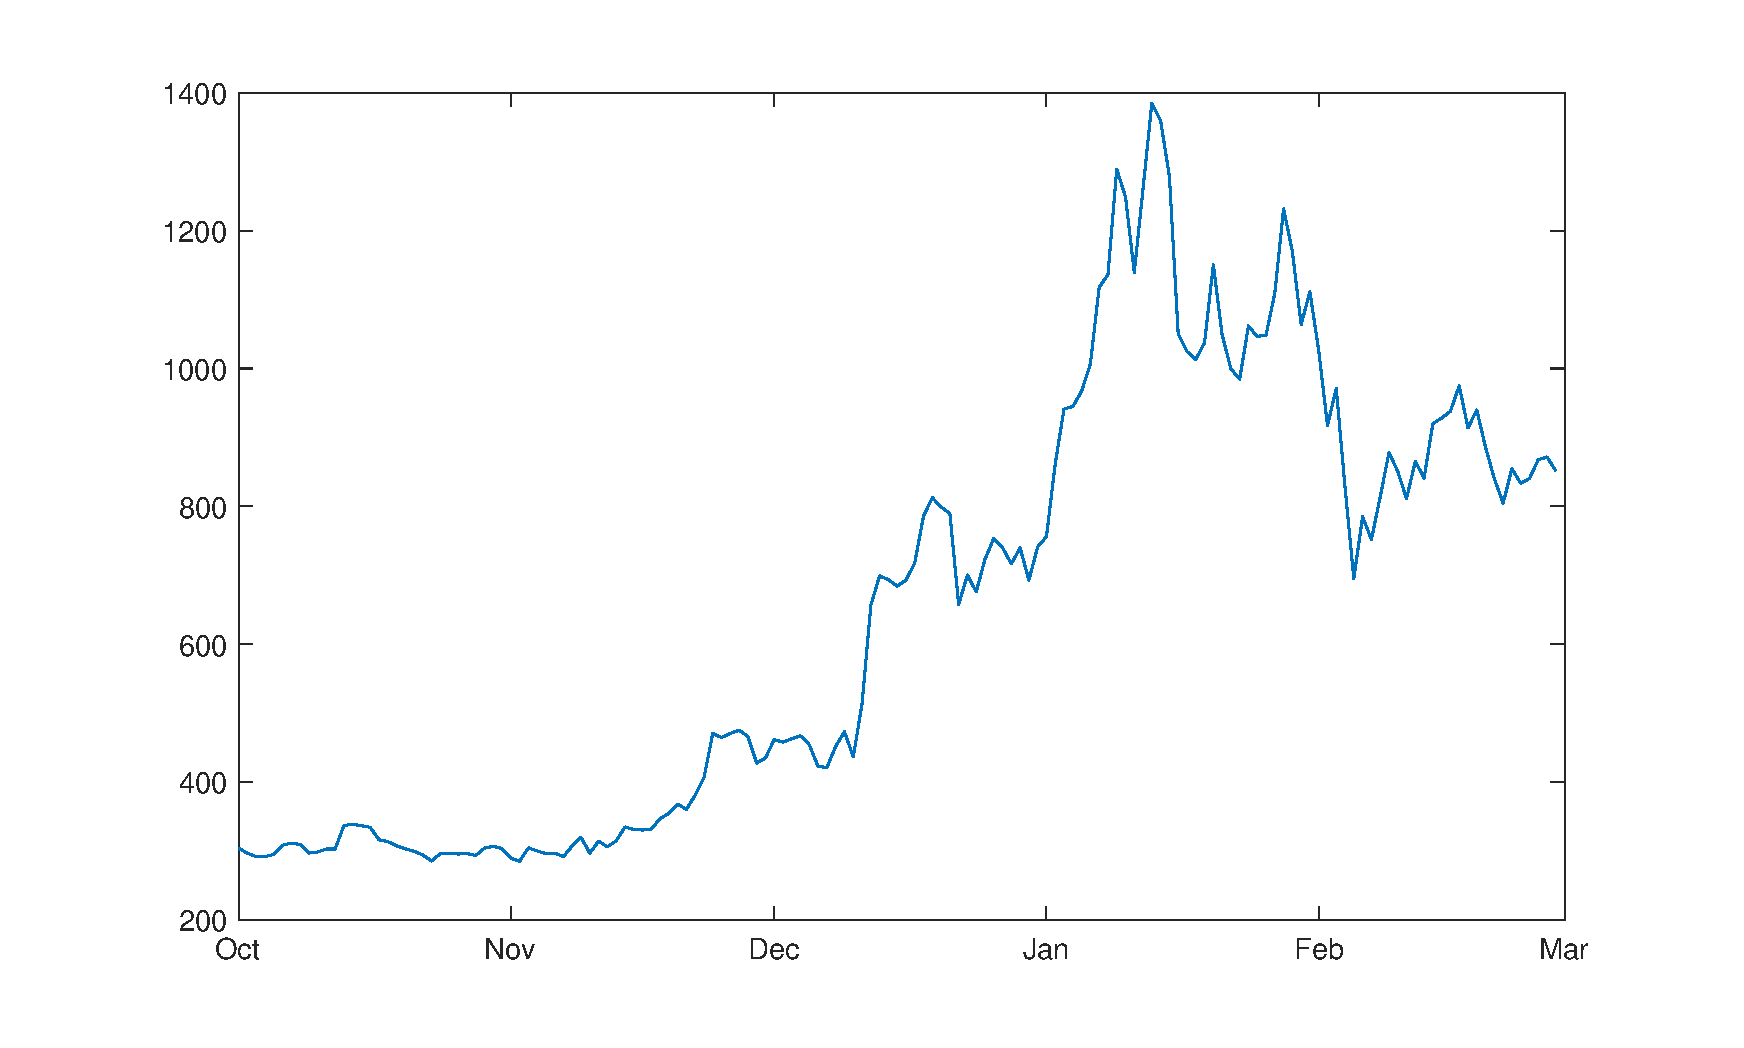
\includegraphics[width=0.95\textwidth]{eth_price}
\par\end{centering}
\caption{ETH/USD Price from 1 Oct 2017 to 28 Feb 2018}\label{fig:ethprice}
\end{figure}


The extremely large volatility means that a cryptocurrency like ETH cannot be used as a reliable means to store value. It is risky to hold the currency even for a single day due to this fluctuation. Even if retailers accept the cryptocurrency for payments, they may have to exchange it immediately into traditional currencies to avoid risk.


% Since their inception, crypto currencies aim to create an alternative financial system comparable to fiat financial systems. In a fiat system, money or credit exists in a few different forms: actual currency in circulation and fixed income assets such as time deposits and money market funds, which are the foundation for the rest of the financial market to build on. The crypto market is at primitive stage as it lacks coins or tokens comparable to fiat money due to their huge price volatility,  and thus there are no established fixed income assets either. However, currently the crypto market is at primitive stage as it lacks coins or tokens comparable to fiat money due to their huge price volatility, and thus there are no established fixed income assets either.

A stable coin is a crypto coin that keeps stable market value against a specific index or asset, most noticeably U.S. dollar. Stable coins are desirable for at least three reasons:
\begin{itemize}
\item They can be used within blockchain systems to settle payments. For example, lawyer or accountants can exchange their stable coins generated by smart contracts automatically for the services they provide within the system, without being bothered by the exchange fees from a cryptocurrency to U.S. dollar, which can range from 0.7\% to 5\%.
\item  They can be used to form crypto money market accounts, for the purpose of doing asset allocation for hundreds cryptocurrencies.
\item They can be used by miners or other people who provide essential services to maintain blockchain systems to store values, as it may be difficult and expensive for them to convert mined coins into traditional currencies.
\end{itemize}
However, as we can see, existing cryptocurrencies are too volatile to be served as stable coins.
In fact, how to create a good stable coin is called the ``Holy Grail of Cryptocurrency'' in the media (Forbes, March 12, 2018,
Sydney Morning Herald, Feb 22, 2018, Yahoo Finance, Oct 14, 2017)





% Tether claims to have 1:1 USD collateral in its centralized bank accounts \cite{USDT}; Basecoin tries to control money supply by playing an algorithmic version of central bank \cite{Basecoin}; MakerDAO uses decentralized over-collateralization to maintain confidence of its Dai stablecoin \cite{MAKERDAO}.


% Most stable token designs to date face a common problem: their holders bear variable levels of counter-party risks, but there is little incentive or even additional cost to hold these tokens. We believe a crypto-token with low price volatility and stable income is a superior safe haven asset and is essential for a more robust crypto market.


There are four existing types of issuance of stable coins. The first type is an issuance backed by accounts in real assets such as U.S. dollars, gold, oil, etc. More precisely, these stable coins represent claims on the underlying assets. For example, Tether coin is claimed to be backed by USD, with the conversion rate  1 Tether to 1 USD (see \cite{tether_tether:_2016}). However, it is very difficult to verify the claim that Tether has enough reserve in U.S. dollar, especially on a daily basis.\footnote{
In fact, U.S. regulators issued a subpoena to Tether on December 6, 2017, on whether \$2.3 billion of the tokers outstanding are backed by U.S. dollars held in reserve (Bloomberg news, January 31, 2018).}
%In fact
%has a major disadvantage: the total assets is about \$62.46 million, but the total liabilities is \$63.014 million, with a negative equity more than half million.
There are other tokens claimed to link to gold (e.g. Digix, GoldMint, Royal Mint Gold, OzCoinGold, and ONEGRAM), although the claims are also hard to verify. Recently in February 2018, the government of Venezuela issued Petro, a cryptocurrency claimed to be backed by one barrel of oil.

The second type is the seigniorage shares system, which has automatic adjustment of the quantity of coin supply: When the coin price is too high, new coins are issued; when the coin price is too low, bonds are issued to remove tokens from circulation. A typical example of this type is Basecoin (see \cite{al-naji_basecoin:_2018}). However, the difficulty of maintaining the right balance of supply and demand of a stable coin is at the same level of difficulty faced by a central bank issuing fiat currency.

The third type is an issuance backed by over-collateralized cryptocurrencies with automatic exogenous liquidation. 
For example, one can generate \$100 worth of stable coins by depositing \$150 worth of Ether. The collateral will be sold automatically by a smart contract, if the Ether price reaches \$110. 
One can also combine the idea of over-collateralization and seigniorage by issuing more coins if the coin price is too high, and allow people to borrow the coin, which gives borrower to buy back the coin if the coin price is too low, thus pushing the price higher. 
Examples of this type include the DAI token issued by MakerDAO; see \cite{makerteam__2017}. A drawback of this type is the relative large collateral size.



The last type is government-backed stable coins. Besides Venezuela, other countries are considering issuing cryptocurrencies, including Russia and China. Canadian government also did Project Jasper involving the ``CAD-coin'', in which a Blockchain network is built for domestic interbank payment settlements. There is a virtual currency working group under the Federal Reserve System in U.S., which uses the ``Fedcoin'' internally. As commented by \cite{garratt_cad-coin_2016}, ``The goal is to create a stable (less price volatility) and dependable cryptocurrency that delivers the practical advantages of Bitcoin even if this means involving the central government and abandoning the Libertarian principles that many believe underlay Bitcoin's creation.''

There are several advantages of issuing stable coins by governments. They are cheaper to produce than the cash in bills or coins, and they are never worn out. They can be tracked and taxed automatically by the blockchain technology. They can facilitate statistical works, such as GDP calculation and collecting consumer data. Furthermore, they can simplify legal money transfers inside and outside blockchains. Finally, as pointed out by \cite{bech_central_2017}, the main benefit of a retail central bank backed cryptocurrency is that it would have the potential to provide the anonymity of cash. The first countries that adopt stable coins will likely see the inflow of money from people who want stable currencies on blockchains.

However, a main drawback of issuing stable coins purely by governments is the cost. More precisely, does a government have enough expertise in maintaining a computer system, is a government willing to put enough reserve to back up a stable coin fully, and  how does a government control supply and demand of a stable coin in a global anonymous blockchain network (which can be quite different from a fiat currency network)?



\subsection{Our Contribution}

We use the option pricing theory (c.f. \cite{duffie_dynamic_2010,hull_options_2017,ingersoll_theory_1987,jarrow_derivative_1999,shreve_stochastic_2004}) to design several dual-class structures that offer entitlements to fixed income stable coins (Class A coins) pegged to a traditional currency as well as leveraged investment opportunities (Class B coins).  The design is inspired by the dual-purpose funds popular in the U.S. and China. More precisely, due to downward resets, a vanilla A coin behaves like a bond with the collateral amount being reset automatically. To reduce volatility, the vanilla A coin can be further split into additional coins, \Ap and \Bp. Unlike traditional currencies, these new class A coins record all transactions on a blockchain without centralized counterparties.

We show that the proposed stable coins have very low volatility; indeed the volatility of class \Ap coin is so low that it is essentially pegged to the U.S. dollar.
Table \ref{tbl:volcomp} reports the volatility of ETH, S\&P 500 index, Gold price, U.S. Dollar index, class A and \Ap coins, respectively.

\begin{table}[!htb]
	\footnotesize
	\centering
	\caption{Annualized Volatility of Our Stable Coins versus Common Market Indices}\label{tbl:volcomp}
	\begin{tabular}{@{}c c c c c c c}
	\toprule
	Index & ETH & S\&P 500 & Gold &  US\$ Index & Class A Coin & Class \Ap Coin \\\midrule
	Volatility & 120.49\% & 13.15\% & 9.44\%  & 5.76\% & 2.37\% & 0.87\%\\
	\bottomrule
	\end{tabular}
	\vspace{0.5em}
	\par\flushleft\footnotesize Annualized volatility is calculated from 1 Oct 2017 to 28 Feb 2018.
\end{table}


The design of stable coins can be used alone in most cases, except in the case of Black Swan events, when the underlying cryptocurrency suddenly drops close to zero within an extremely short time period.\footnote{The intuition here is similar to that of the risk of the top tranche of a CDO contract. If the correlations of all firms covered within the CDO are close to 1, then one firm's default leads to almost all other firms' default, resulting in a significant drop of the top tranche value.} Therefore, to be truly stable, stable coins need a guarantee in Black Swan events.




A policy implication of this paper is that a public-private partnership may be formed to issue stable coins backed by a government. More precisely, by designing a set of stable coins using the option pricing theory via private market forces, the government only needs to back up the stable coins in extreme cases of Black swan events, just like what the U.S. government does for the FDIC insurance for private money market accounts in U.S.


%When combined with insurance from a government, similar to FDIC insurance, our design can also serve as a basis for issuing a sovereign cryptocurrency via a private-public partnership. By doing so, the government can let the private sector do the job of issuing stable coins, except to provide insurance in rare cases, saving government human and financial resources.


\subsection{Literature Review}

Although our design of stable coins is inspired by dual-purpose funds, it is different from dual-purpose funds in U.S. and China in the aspects shown in Panel A of Table \ref{tbl:difference}. These differences require a different modeling, which is summarized in Panel B of Table \ref{tbl:difference}.

\begin{table}[!htb]
\centering
	\caption{Contract and Model Comparison of Our Stable Coins and Dual-Purpose Fund in U.S. and China}\label{tbl:difference}
	\vspace{1em}
	\scriptsize
	\begin{tabularx}{0.88\linewidth}{@{}c c c c c c@{}}
	\toprule
	\multicolumn{6}{l}{\bf Panel A: Contract Comparison}\\ \midrule
		& \begin{tabular}{@{}c@{}}Payment Style\\ of A Share\end{tabular} & \begin{tabular}{@{}c@{}}Payment Style\\ of B Share\end{tabular} & \begin{tabular}{@{}c@{}} Reset \\ Barriers \end{tabular} & Lifespan & \begin{tabular}{@{}c@{}}Underlying\\ Asset\end{tabular} \\ \midrule
	\begin{tabular}{@{}c@{}}Dual-Purpose\\ Fund in U.S.\end{tabular} & Dividend & \begin{tabular}{@{}c@{}}Single payment\\ at wind-up date\end{tabular}  & No & Finite & \begin{tabular}{@{}c@{}}Stock/\\ Stock Index\end{tabular}\\ \midrule
	\begin{tabular}{@{}c@{}}Dual-Purpose\\ Fund in China\end{tabular} & Fixed Income &  \begin{tabular}{@{}c@{}c@{}}Payments affect \\  the underlying\\ asset but not\\ the exchange ratio\end{tabular} & Yes & Infinite & Stock Index\\ \midrule
	\begin{tabular}{@{}c@{}}Our Vanilla\\ A and B Coins\end{tabular} & Fixed Income & \begin{tabular}{@{}c@{}c@{}}Payments affect \\ the exchange ratio
	\\but not the \\underlying asset \end{tabular} & Yes & Infinite & \begin{tabular}{@{}c@{}}USD denominated\\ cryptocurrency \end{tabular}\\
	\bottomrule \addlinespace[8pt]
	\end{tabularx}
	\begin{tabularx}{0.88\linewidth}{@{}c p{30pt} c@{}}
	\multicolumn{2}{l}{\bf Panel B: Model Comparison}\\
	\midrule
		& & Pricing Model\\ \midrule
		\begin{tabular}{@{}c@{}}Dual-Purpose Fund in U.S. \\\cite{ingersoll_theoretical_1976} \\\cite{jarrow_primes_1989}\end{tabular} & & Black-Scholes PDE\\ \midrule
		\begin{tabular}{@{}c@{}}Dual-Purpose Fund in China\\ \cite{dai_overpricing_2018}\end{tabular} & & \begin{tabular}{@{}c@{}} Periodic PDE, constant upper barrier\end{tabular}\\ \midrule
		\begin{tabular}{@{}c@{}}Our Vanilla A and B Coins\end{tabular} & & \begin{tabular}{@{}c@{}} Periodic PDE, time-dependent upper barrier\end{tabular}\\
	\bottomrule
	\end{tabularx}
	\vspace{0.5em}
	\par\flushleft\scriptsize The dual-purpose funds in U.S. include those studied in \cite{ingersoll_theoretical_1976} and the prime and scores studied in \cite{jarrow_primes_1989}.
\end{table}


The blockchain technology behind cryptocurrencies can create significant economic benefits in many applications.  \cite{cong_blockchain_nodate} showed that the blockchain technology can provide and maintain ``decentralized consensus'', which improves the functioning of the whole system, reduces information asymmetry, and enhances competition. \cite{yermack_corporate_2017} pointed out that blockchains may offer to corporation shareholders lower trading costs and more visible ownership records and transfer of shares. \cite{malinova_market_2017} designed a financial market based on the blockchain technology that can give investors alternative ways of managing the visibility of their holdings and trading intentions.


%\subsection{Pros and Cons of Cryptocurrencies}

There are many papers and media articles discussed pros and cons of cryptocurrencies.
Using cryptocurrencies as a payment method has several benefits. First, as pointed out in \cite{harvey_cryptofinance_2016}, the core innovation of cryptocurrencies like Bitcoin is the ability to publicly verify ownership, instantly transfer the ownership, and to do that without any trusted intermediary. Therefore, cryptocurrencies reduce the cost of transferring ownership. Also, the blockchain technology makes the ledger easy to maintain, reduces the cost of networking (see \cite{catalini_simple_2016}), and is robust against attackers.\footnote{Indeed, an attacker needs to race with his CPU power against the whole system; if he fails behind in the beginning, the probability of his catching up diminishes exponentially as the race goes on (see \cite{nakamoto_bitcoin:_2008} and  \cite{Grunspan_2018}).} The distributed ledger can result in a fast settlement that reduces counterparty risk and improves market quality (see \cite{khapko_smart_2018}). Furthermore, since the transaction is recorded to the blockchain anonymously, cryptocurrencies help to protect the privacy of their users. The underlying technology of cryptocurrencies may one day strengthen the menu of electronic payments options, while the use of paper currency is phased out (see \cite{rogoff_costs_2015}).



There are also some criticisms of cryptocurrencies. First, a payment system with cryptocurrencies lacks a key feature, the confidence that one can get his money back if he is not satisfied with the goods he purchased. As pointed out in \cite{grinberg_bitcoin:_2011}, Bitcoin is unlikely to play an important role in the traditional e-commerce market, since consumers typically do not care about the anonymity that Bitcoin provides; instead, they prefer a currency they are familiar with for most goods and services, and they want fraud protection.  Second, unlike government-backed systems, Bitcoin does not have identity verification, audit standards, or an investigation system in case something bad happens. For instance, one may lose all his deposit in cryptocurrencies should his password get stolen, and there is no remedy. Furthermore, Blockchain systems are not as trustworthy as they seem to be. Without an intermediate, individuals are responsible for their own security precautions. Finally, it is difficult to value cryptocurrencies like Bitcoin\footnote{By considering the equilibrium in the case where Bitcoin is the only currency in the economy and the case with two currencies, \cite{garratt_bitcoin_2018} found that the value of Bitcoin lies upon self-fulfilling beliefs, and the set of beliefs that can be self-fulfilling needs to be huge.}.

Here we want to point out that despite significant drawbacks of cryptocurrencies, it is generally agreed that the blockchain technologies are here to stay. However, blockchain technologies automatically generate cryptocurrencies for the purpose of charging the services provided by the system (such as fees incurred by all programming codes which are run on the Ethereum network), crediting essential services to the system (such as the verification services provided by miners\footnote{\cite{ehb2017} and \cite{hlm2017} study mining fees on the Bitcoin system.}), and of exchanging credits for services. Therefore, cryptocurrencies will not disappear as long as blockchain technologies exist. Thus, designing suitable stable coins is essential for the blockchain system to perform financial functions efficiently and for doing asset allocation across different cryptocurrencies generated by different blockchain systems. In this regard, governments can provide an essential role in helping design a better financial ecosystem of blockchains.

% The rest of paper is organized as follows. The design of stable coins is presented in Section \ref{sec:Product-Design}, while the valuation of these coins is given in Section \ref{sect:valuation}. Numerical examples are given in Section \ref{sect:numerical}. Further design details and extension of A0 and A1 coins are given in appendices, along with technical theorems and propositions.




% \subsection{Risk Segmentation}

% In the fiat market, risk segmentation exists in every level of market. At asset class level, risk averse investors choose fixed income products while risk seeking investors choose equity or commodity. Within the fixed income market, conservative investors choose safe haven assets such as government bonds while aggressive players choose high yield bonds, or otherwise known as junk bonds.

% Although most of crypto assets are considered highly speculative, there still exist different segments of risk appetites. The existence of margin trading in exchanges like BitFinex and Huobi Pro demonstrates the need of leverage from aggressive crypto investors. Similarly, safe haven assets providing low volatility and stable income will be appealing to institutional players, short-term pessimistic investors and ICO project teams. However, to our best knowledge, there is no viable product at the moment.

% The price volatility cannot be eliminated, but can be transferred. Through a structured contract, a risk-seeking investor can get exposed to higher leverage with limited assets, while a risk-averse investor can avoid unwanted price fluctuations by entering the other side of the contract. The financial market has created many products satisfying different risk segments, some of which can be very practical for crypto market participants.

% \subsection{Leveraged Funds}

% Leverage is the strategy of using borrowed capital to increase the potential return of an investment \cite{Leverage}. Retail investors have less access to leverage methods such as margin loans and financial derivatives, which promotes the creation of leveraged fund products.

% An interesting class of leveraged funds is the dual-purpose funds, also known as primes and scores, which are mutual funds that are split into two classes of shares by design: low risk shares and high risk shares. They were designed to provide investors with the opportunity of repackaging their investment incomes and capital flow in accordance with their preferences. Dual-purpose funds first appeared in U.S. in 1965, but faded out in early 1990s due to a change in the tax code that resulted in double taxation \cite{DM2018}. The valuation of dual-purpose funds in U.S. was investigated theoretically and empirically in \cite{Ingersoll1976} and \cite{JO}.

% The dual-purpose fund was introduced in China in 2010 and it quickly became one of the most popular leveraged products there, reaching market size of 500 billion CNY (80 billion USD) at its peak. A Chinese dual-purpose fund usually takes an open-end index-tracking fund as underlying and has two classes of shares: the low risk A shares behave like a perpetual bond with periodical coupon payments, and the high risk B shares are essentially a closed-end fund magnifying the exposure of the underlying index. A set of upward and downward reset clauses is imposed to reduce the risk of both shares \cite{DM2018}.

% We are inspired by the Chinese dual-purpose fund for three reasons: (i) both the income and leveraged shares answer unfulfilled demands of crypto-currency investors; (ii) the market mechanism, pricing formula, and arbitrage method prove to work in real market; and (iii) the structure can be efficiently implemented by Smart Contracts.

% \subsection{Smart Contract}


% Up until now, the most popular stablecoin solution has been issuer-backed assets. And it is almost a market consensus that such issuers are not always trustworthy. We agree with Ethereum authors' argument that, a decentralized market of speculators and arbitragers powered by smart contract, could be an alternative solution.

% This paper aims to propose an alternative approach of creating stable value tokens, providing a different set of trade offs between price stability, holder incentive and supply flexibility. We believe the solution will be very useful for broader adoption of the crypto market.


\section{Product Design}\label{sec:Product-Design}
%\begin{flushright}
%{\small{}Everything should be made as simple as possible, but no simpler.
%}\\
%{\small{}\textendash{} }\emph{\small{}Albert Einstein}
%\par\end{flushright}{\small \par}
In this section, we introduce the detailed design of our stable coin, including its creation/redemption and its cash flow. We also point out several differences between the product and the dual-purpose funds in U.S. and in China.

\subsection{Vanilla Class A and B Coins}\label{subsect:vanilla}

Our stable coin has a dual-class split structure which, combined with smart contract rules and market arbitrage mechanism, provides the holders of each class with principal-guaranteed fixed incomes and leveraged capital gains, respectively. The Class A Coin behaves like a bond and receives periodical coupon payments. The Class B Coin entitles leveraged participation of the underlying cryptocurrency. Simply put, this split structure means that the holders of Class B coins borrow capital from the holders of Class A coins and invest in a volatile cryptocurrency. Furthermore, a set of upward and downward reset clauses is imposed, where downward resets reduce default risk of Class B to protect Class A, and upward resets ensure a minimum leverage ratio of Class B to make Class B attractive to leverage investors.

For illustration we choose ETH as the underlying cryptocurrency, and the initial leverage ratio is set to $2$.\footnote{The design of a contract with a general initial leverage ratio is discussed in Appendix \ref{subsec:General-Product-Design}.} Class A and B coins can be created by depositing ETHs to a custodian smart contract.\footnote{A custodian smart contract can perform multiple tasks that facilitate key mechanism of the system, including: creation and redemption of the stable coin, safekeeping the underlying digital assets (e.g. ETH), calculation of stable coins' net values, and execution of Reset events. The deposited underlying cryptocurrency is kept by the custodian smart contract, as collateral of the Class A and Class B coins issued by the contract. Any user or member of the public can verify the collateral and coins issued through third party applications such as \href{http://etherscan.io}{Etherscan.io}.} Upon receiving two shares of underlying ETH at time $t$, the Custodian contract will return to the depositor $\beta_t P_0 $ of Class A and Class B coins each, where $P_{0}$ is the initial price of underlying ETH in USD at the inception of the coins ($t=0$), and $\beta_t$ is the time-$t$ conversion factor. We set $\beta_0=1$, which means that two shares of ETH can initially exchange for $P_0$ shares of Class A and Class B each. The conversion factor $\beta_t$ changes only on upward/downward resets or regular payout dates, and the change rule will be introduced later. To withdraw ETH at time $t$, holders of Class A and Class B coins can send, e.g., $\beta_t P_0$ shares of Class A and Class B coins each to the Custodian contract, then the contract will deduct the same amount of Class A and Class B coins, and return to the sender two ETHs.
For instance, if the initial ETH/USD price is 500 and $\beta_t=1$, then two shares of ETH can create 500 shares of Class A coins and Class B coins each, and 500 shares of Class A and B coins each can be redeemed into two shares of ETH. Figure \ref{fig:initial} illustrates this split structure.

\begin{figure}[!htb]
	\centering
	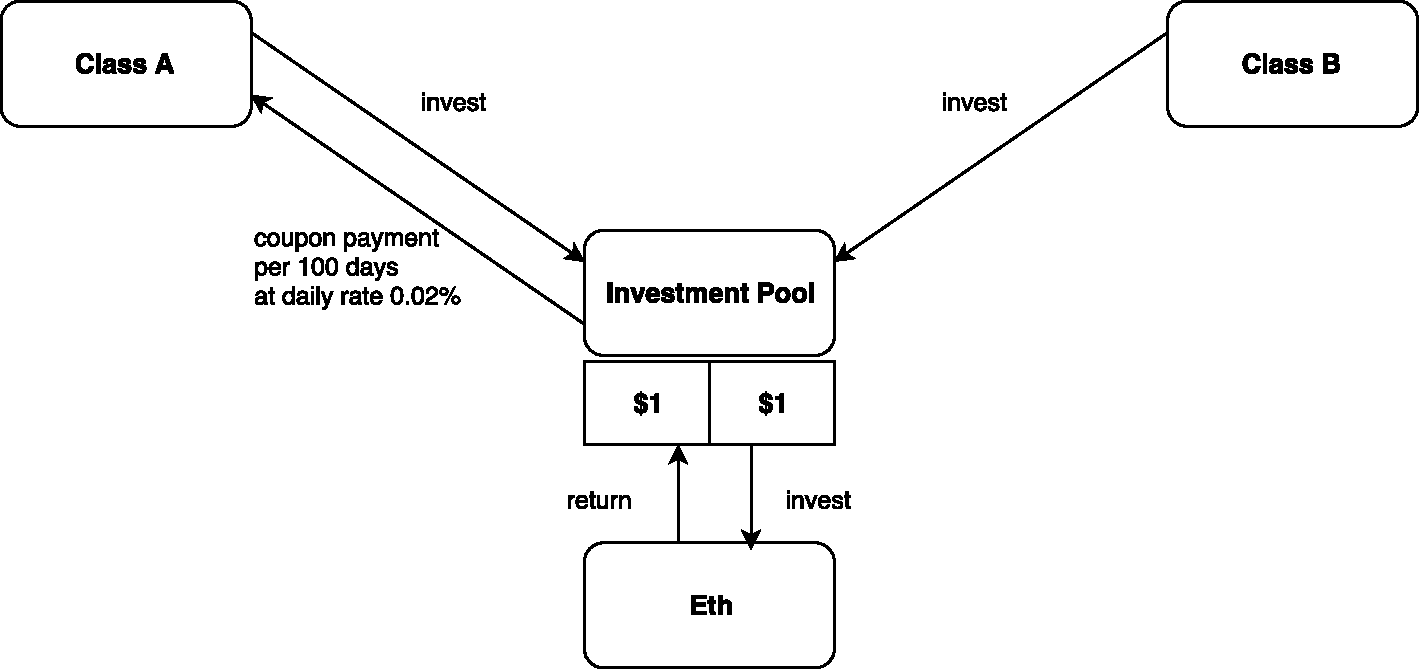
\includegraphics[width=0.8\textwidth]{initial}
	\caption{Class A and B, Initial Split. At time $t$, one share of Class A and B each invests \$1 in ETH. The initial ETH price is $P_0=\$500$, and the prevailing conversion factor $\beta_t=1$. So two shares of ETH exchange for 500 shares of Class A coins and 500 shares of Class B coins.}\label{fig:initial}
\end{figure}

To describe the cash flow of Class A and B coins, we introduce the net asset dollar values of Class A and B coins, $V_A$ and $V_B$. Thanks to the exchange between ETH and Class A/B coins, the following parity relation holds at any time:
\begin{equation}
\label{parity}
V_{A}^{t}+V_{B}^{t}=\frac{2P_{t}}{\beta_tP_{0}},
\end{equation}
where $P_t$ is the prevailing price of underlying ETH in USD.
The net asset value of Class A coins at time $t$ is defined as
\begin{equation}
V_{A}^{t}= 1+R\cdot v_t, \label{eq:netvalue}
\end{equation}
where $R$ is the \emph{daily} coupon rate, and $v_t$ is the number of days from the inception, last reset, or last regular coupon payout date. The above design ensures that the initial net asset values of Class A and B coins are both equal to one dollar.

\subsubsection{Regular Payout}
Assume regular coupons are paid every $T$ days. When $v_{t-}=T$, i.e., $V_{A}^{t-}=1+RT$, a regular payout is triggered, then the holder of each Class A coin receives payment with dollar value $RT$,\footnote{Payments are made in the form of underlying ETH from the Custodian contract. For instance, upon regular payout, the holder of each Class A coin receives underlying ETH with amount $\frac{RT}{P_{t}}$.}
 and the net asset value of Class A resets to \$1, namely, $V_{A}^{t+}=1$. Since no cash flow occurs for Class B coin upon regular payout, the net asset value of Class B remains unchanged, that is, $V_{B}^{t-}=V_{B}^{t+}$. Noting that the parity relation (\ref{parity}) always holds across regular payout, we deduce that the conversion factor $\beta$ experiences a jump upon regular payout:
 $$\beta_{t+}=\frac{2P_{t}}{2P_{t}-\beta_{t-}P_{0} RT}\beta_{t-}.$$
 For instance, assuming $R=0.02\%$, $T=100$, and $P_0=\$500$, a regular coupon payout occurs at time $t$ when $P_t=\$450$ and $\beta_{t-}=1$, then Class A receives \$0.02 coupon payment, and the conversion ratio is reset to $\beta_{t+}=1.011$, which indicates that two shares of ETH can exchange for 505.62 shares of Class A and 505.62 shares of Class B after the regular payout. This is illustrated in Figure \ref{fig:regular}.


\begin{figure}[!htb]
	\centering
	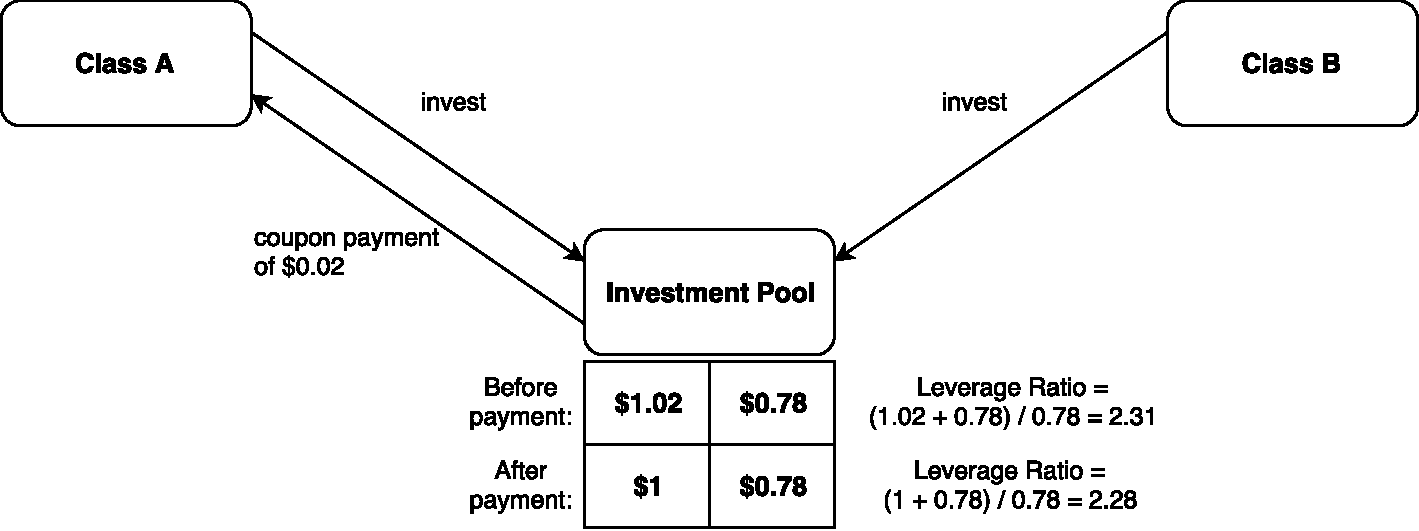
\includegraphics[width=0.8\textwidth]{periodic}
	\caption{Class A and B, Regular Payout. After 100 days, the ETH price drops to \$450, so that total investment of one Class A coin and one Class B coin becomes \$1.8, within which \$1.02 belongs to Class A. A regular payout takes place, and Class A receives \$0.02 coupon payment. New exchange ratio: 2 shares of ETH now correspond to 505.62 ($=500\times\frac{2\times450}{2\times450-500*0.02}$) shares of Class A and 505.62 shares of Class B, yielding $\beta_{t+}=1.011$.}\label{fig:regular}
\end{figure}

\subsubsection{Upward Reset}
An upward reset is triggered when the net asset value of Class B coins reaches the predetermined upper bound, denoted by $\mathcal{H}_{u}$. On an upward reset time $t$, net asset value of both classes resets to 1 USD, Class A and B's holders will receive payments of value $V_{A}^{t}-1$ and $V_{B}^{t}-1$, respectively, and conversion factor $\beta_{t+}$ is reset to $P_t/P_0$ so that after the upward reset two shares of ETH can exchange for $P_t$ share of class A and B. For instance, as illustrated in Figure \ref{fig:upward}, after another 50 days, the ETH price grows to \$760.96, so the net asset value of the Class B grows to $\mathcal{H}_{u}\equiv \$2$, triggering an upward reset. The holders of Class A and B receive payments with amount \$0.01 and \$1, respectively. Two shares of ETH now correspond to 760.96 shares of Class A and 760.96 shares of Class B, yielding $\beta_{t+}=1.52$.

\begin{figure}[!htb]
	\centering
	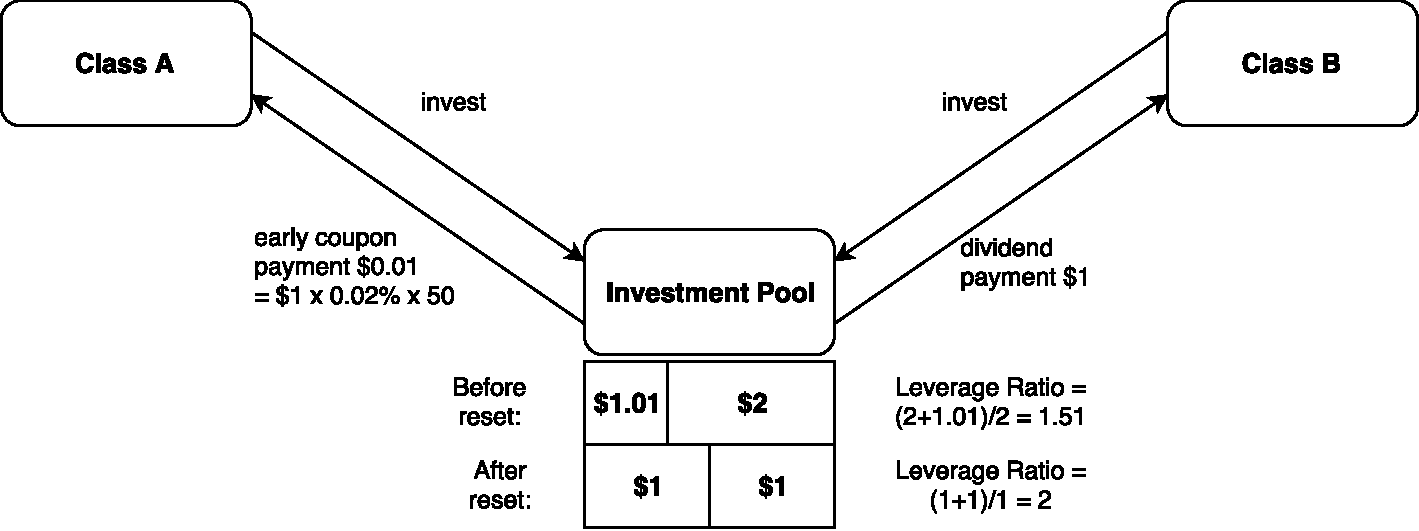
\includegraphics[width=0.8\textwidth]{upward}
	\caption{Class A and B, Upward Reset. After 50 days, the ETH price grows to \$760.96, and Class B NAV grows to \$2, triggering an upward reset. Class A NAV equals \$1.01, where \$0.01 is 50-day accrued coupon. On this date, Class A receives \$0.01 coupon payment, and Class B receives \$1 dividend payment. New exchange ratio: 2 shares of ETH now correspond to 760.96 shares of Class A and 760.96 shares of Class B, yielding $\beta_{t+}=760.96/500=1.52$. }\label{fig:upward}
\end{figure}

\subsubsection{Downward Reset}
 A downward reset is triggered when the net asset value of Class B coins reaches the predetermined lower bound, denoted by $\mathcal{H}_{d}$,  On a downward reset time $t$, Class A holders receive a payment with dollar value $V_{A}^{t}-\mathcal{H}_{d}$, and  $1/\mathcal{H}_{d}$ shares of Class A and B are merged into one share of Class A and B, respectively, so that the net asset value of both classes resets to \$1. The conversion factor $\beta_{t+}$ resets to $P_t/P_0$, that is, two ETHs can exchange for $P_t$ shares of Class A and B after the reset. For instance, as illustrated in Figure \ref{fig:downward}, after another 50 days, the ETH price drops to \$479.40, so that the net asset value of Class B drops to $\mathcal{H}_{d}\equiv \$0.25$, triggering a downward reset. Class A receives \$0.01 coupon payment and \$0.75 principal payback, and then both classes undergo a 4:1 merger. Two shares of ETH now correspond to 479.40 shares of Class A and 479.40 shares of Class B, yielding $\beta_{t+}=479.40/500=0.96$.

 Under a black swan event, the net asset value of Class B coins $V_B^t$ is likely lower than $\mathcal{H}_{d}$ or even becomes negative upon downward reset. In the case of $V_B^t>0$, we can simply replace $\mathcal{H}_{d}$ by $V_B^t$ for the above description of cash flow and operations on downward reset. If $V_B^t\leq 0$, then both classes are fully liquidated, the holders of Class B receive nothing, and the holders of Class A receive the payment $V_A^t-|V_{B}^{t}|$.

\begin{figure}[!htb]
	\centering
	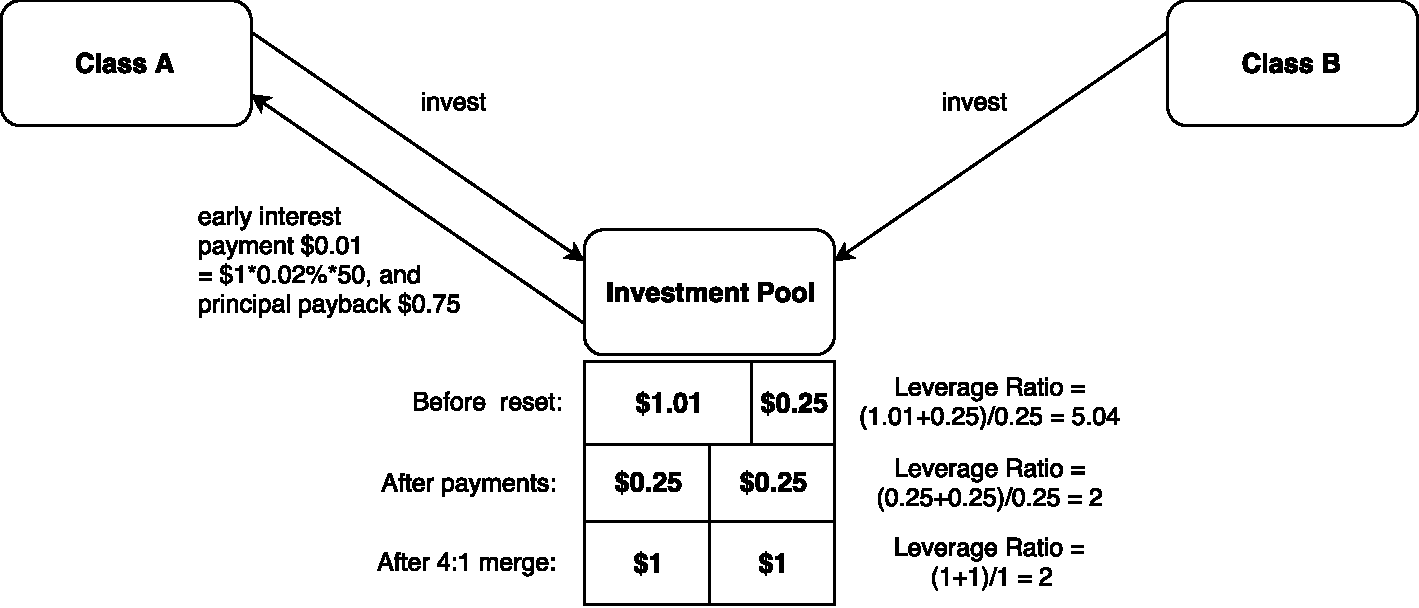
\includegraphics[width=0.8\textwidth]{downward}
	\caption{Class A and B, Downward Reset. After another 50 days, the ETH price drops to \$479.40, and Class B NAV drops to \$0.25, triggering an downward reset. Again, Class A NAV equals \$1.01, where \$0.01 is 50-day accrued coupon. On this date, Class A receives \$0.01 coupon payment, as well as \$0.75 principal payback. Then, Class A and B each undergo a 4:1 merger, so that both have NAV equal to \$1. New exchange ratio: 2 shares of ETH now correspond to 479.40 shares of Class A and 479.40 shares of Class B, yielding $\beta_{t+}=0.96$.}\label{fig:downward}
\end{figure}

{\it No arbitrage} implies that the market prices of Class A and B coins also satisfy the parity relation:
$$W_A^t +W_B^t=\frac{2 P_t}{\beta_t P_0},$$
where $W_A$ and $W_B$ are the market prices of the Class A and B coins, respectively. This has an interesting implication: Suppose the demand of Class B coins is low, then the market value of Class B coins would be low, and the above parity relation implies that the market value of the Class A coins would be high.


Class A coin behaves like a bond. Although Class A has a fixed coupon rate and its coupon payment is periodic and protected by the downward resets, its value is still volatile on non-coupon dates.
%The main risk of Class A is caused by a downward reset, instead of the credit risk of class B.
This is because the coupon rate is usually higher than the risk-free rate, and on a downward reset, a portion of Class A coin will be liquidated, then the holder of Class A will lose high coupons that would be generated from this portion. Therefore, a potential downward reset will make the price of Class A volatile. We will propose two types of more stable coins: \Ap coins (Section \ref{subsect:Ap}) and A0 coins (see Appendix \ref{sect:A0}).


\begin{figure}[p]
\centering
	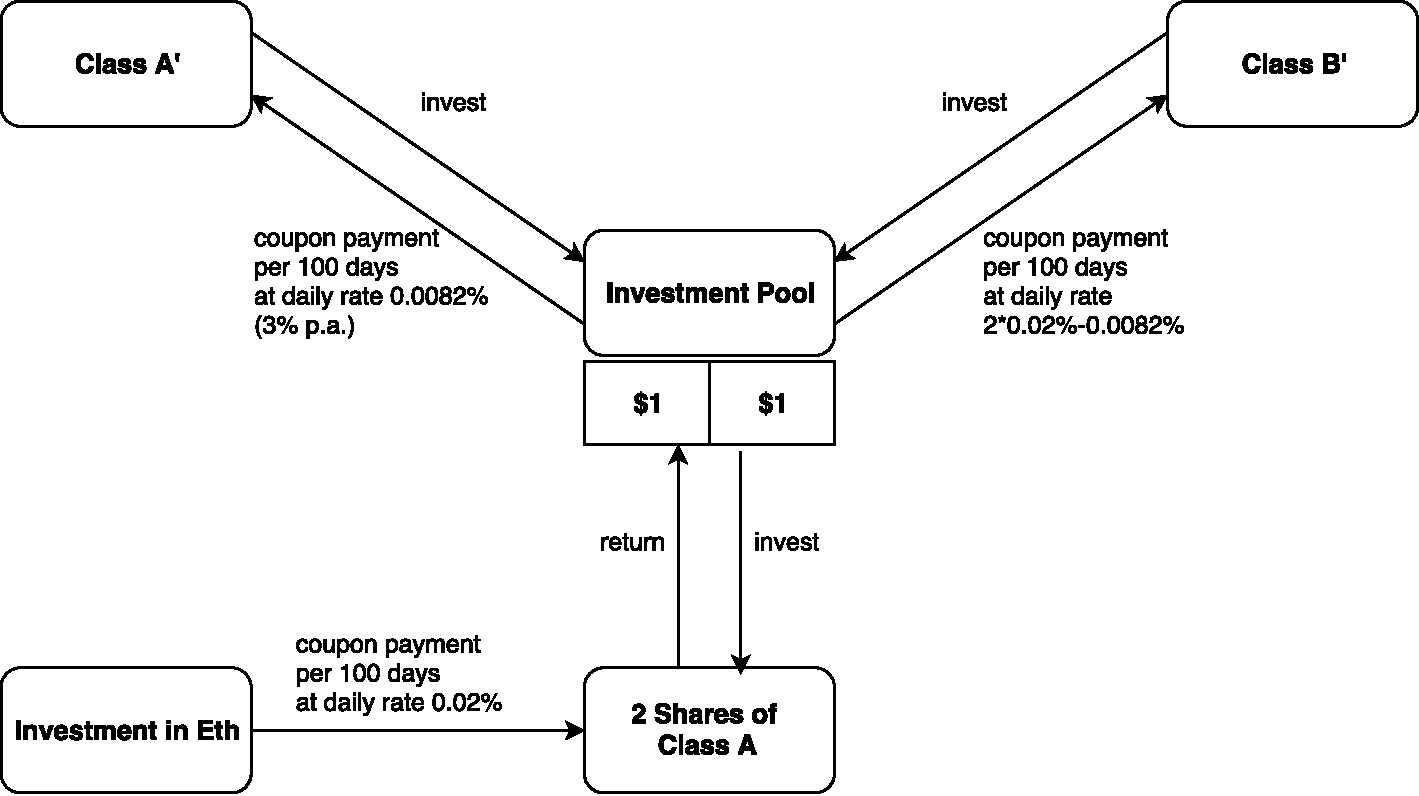
\includegraphics[width=0.7\textwidth]{Ap_periodic}
	\vspace{1em}
	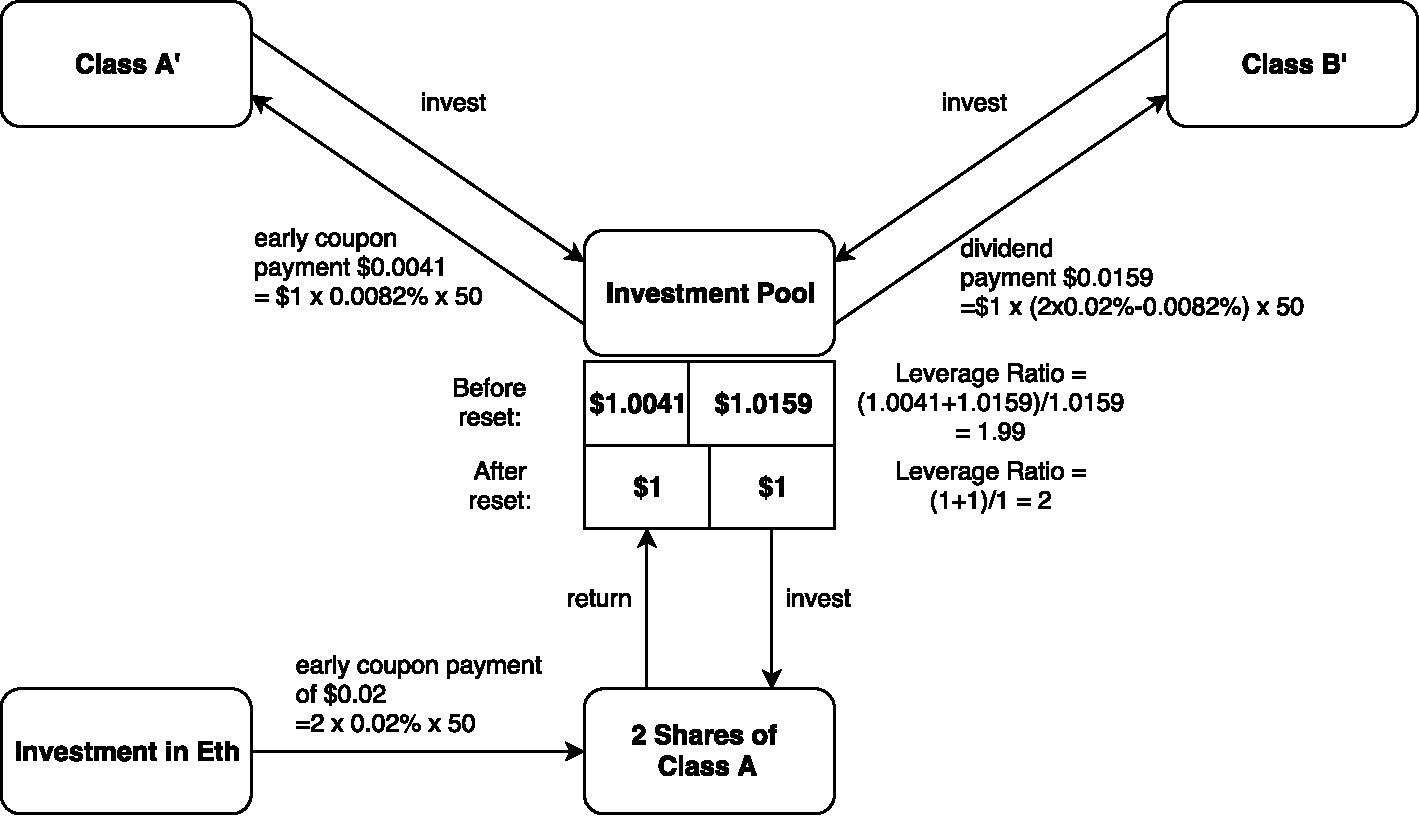
\includegraphics[width=0.7\textwidth]{Ap_upward}
	\vspace{1em}
	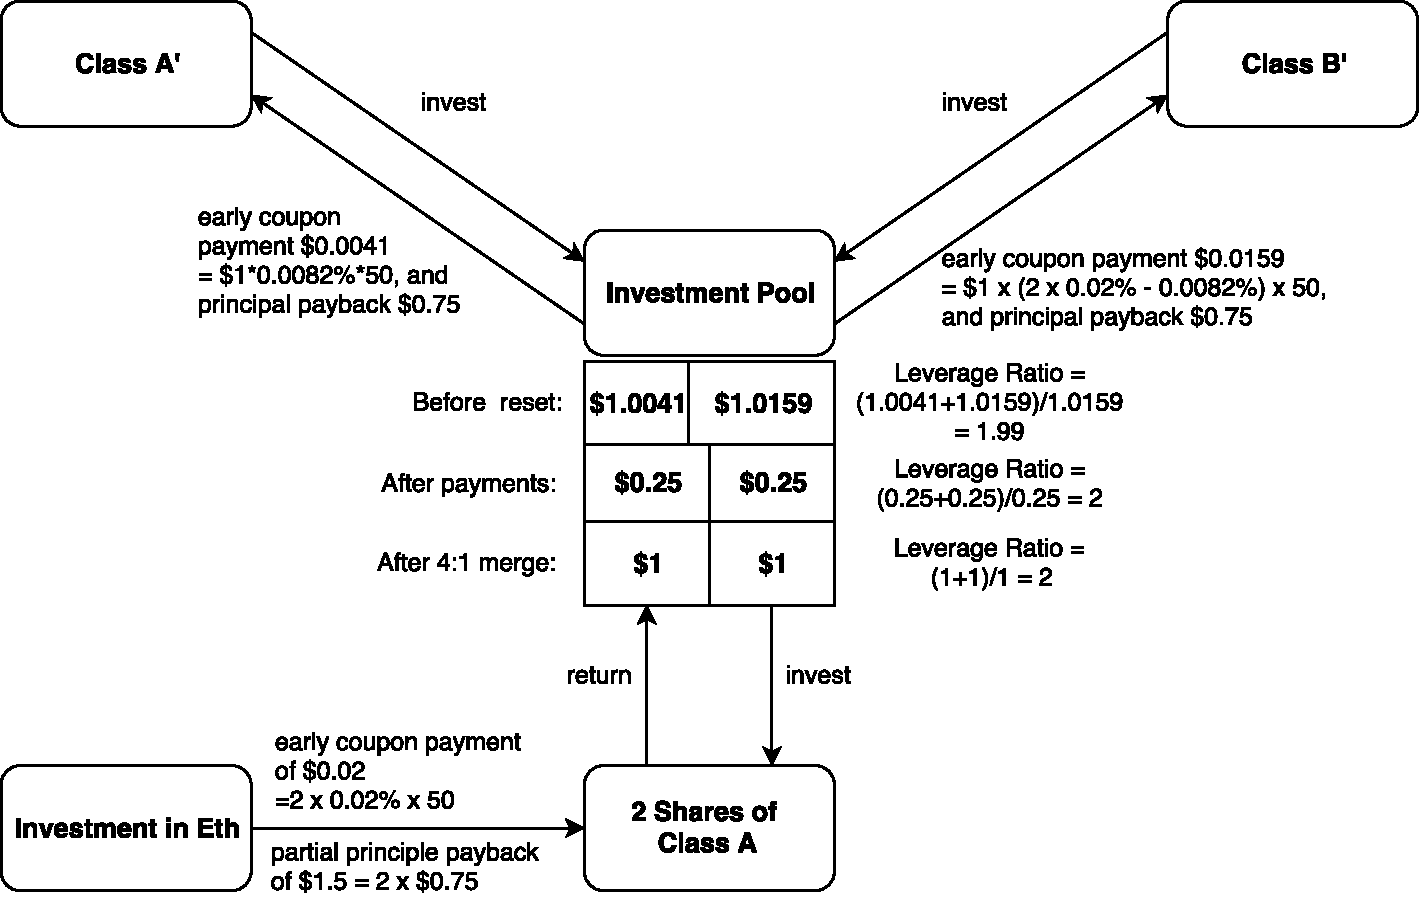
\includegraphics[width=0.7\textwidth]{Ap_downward}
	\caption{{\bf Top Figure:} What happens to Class \Ap on a regular payout date of A. On regular payout dates for Class A (per 100 days), 2 shares of A receives coupon payment \$0.04, i.e. at daily rate 0.02\%. \$0.0082 is paid to \Ap and \$0.0318 to \Bp. {\bf Middle Figure:} Upward Reset of Class \Ap. After 50 days, Class B's net asset value grows to \$2, triggering an upward reset. {\bf Bottom Figure:} Downward Reset of Class \Bp. After another 50 days, Class B's net asset value drops to \$0.25, triggering an downward reset. }\label{fig:Ap}
\end{figure}



\subsection{\texorpdfstring{Class \Ap and \Bp Coins}{Lg}}\label{subsect:Ap}
This extension splits Class A into two sub-classes: Class \Ap and \Bp. Both classes invest in Class A coins. At any time, two Class A coins can be split into one Class \Ap coin and one Class \Bp coin. Conversely, one Class \Ap coin and one \Bp coin can be merged into two Class A coins. The split structure for Class \Ap and \Bp resembles that for Class A and B: Class \Bp borrows money from Class \Ap at the rate $R^\prime$ to invest in Class A. Here $R^\prime$ is set to be close to the risk-free rate $r$, whereas the rate $R$ for Class A is generally much higher.

Class \Ap and \Bp resets {\it when and only when} Class A resets or gets regular payout. Class \Ap gets coupon at the rate $R^\prime$ on regular payouts, upward and downward reset (provided that the net asset value of Class B is positive then), and Class \Bp gets coupon at the rate $2R-R^\prime$ on upward reset. On downward resets, each share of both Class \Ap and \Bp is reduced to $(V_B^t)^+$ share, and Class \Ap gets the value of the liquidated shares (i.e., $1-(V_B^t)^+$ shares). In the extreme case where $V_B^t\le 0$, then both Class \Ap and \Bp are fully liquidated, and \Ap receives its full net asset value $1+R^\prime t$, or the remaining total asset for \Ap and \Bp, $2(1+Rt-|V_B^t|)$, whichever is smaller. Class \Ap behaves like a money market account, except in extreme case, when the underlying asset suddenly jumps (not smooth transit) to close to zero. Using the same example as in Section \ref{subsect:vanilla}, Figure \ref{fig:Ap} illustrates the cash flow of Class \Ap and \Bp coins.





% \subsection{Market Mechanism}
% % \begin{flushright}
% % {\small{}Arbitrage human nature. It's not going to change any time
% % soon. }\\
% % {\small{}\textendash{} }\emph{\small{}James O'Shaughnessy}
% % \par\end{flushright}{\small \par}

% \subsubsection{Premium and Discount}\label{subsec:Premium-and-Discount}

% Like all fixed income products, Class A is expected to trade on premium or at discount with respect to its net value, depending on market condition. When Class A trades on premium, that generally indicates a higher demand for income over leverage and thus Class A buyers are getting lower yield. On the contrary, when Class A trades at discount, that implies a higher demand for leverage over income and thus Class A buyers are paying less and getting higher yield. In an orderly market, Class A's market price can be used to derive the current market cost of funding. As net values draw closer to resets, Class A might trade closer to its net value as traders start exploiting arbitrage opportunities.

% \subsubsection{Market Arbitrage }

% The dual class tokens are two-way fungible to the underlying token (i.e. ETH). Thus, a price parity shall hold as below:
% \[
% P_{A}^{t}+P_{B}^{t}=V_{A}^{t}+V_{B}^{t}\ ,
% \]
% where $P_{A}^{t}$ is the current price of Class A in USD, and $P_{B}^{t}$ is the current price of Class B in USD.

% Along with Equation (\ref{eq:netvalue}) in Section \ref{subsec:Creation-and-Redemption}, the following relation should hold:
% \[
% P_{A}^{t}+P_{B}^{t}=2\cdot\frac{P_{t}}{P_{0}\cdot\beta}\ .
% \]
% On open market, arbitrage opportunity exists when Class A and Class B tokens trade away from their net values and the above equation is likely violated on either side.

%\paragraph{Arbitrage via Creation}
%
%When combined market price of Class A and Class B tokens are higher than their combined net values, i.e.
%\[
%P_{A}^{t}+P_{B}^{t}>2\cdot\frac{P_{t}}{P_{0}\cdot\beta}\ ,
%\]
%arbitrage profit can be exploited by perform DUO token creation:
%\begin{enumerate}[1)]
%\item Buy 1 underlying tokens from open market for $P_{t}$ USD equivalent.
%\item Send the underlying tokens to the Custodian contract.
%\item Based on Equation (\ref{eq:creation}), receive $\frac{P_{0}\cdot\beta}{2}$ Class A and $\frac{P_{0}\cdot\beta}{2}$ Class B tokens.
%\item Sell Class A and Class B tokens on open market for $P_{0}\cdot\beta\cdot\frac{P_{A}^{t}+P_{B}^{t}}{2}$ USD equivalent.
%\end{enumerate}
%The expected payoff of above operations is:
%\[
%P_{0}\cdot\beta\cdot\frac{P_{A}^{t}+P_{B}^{t}}{2}-P_{t}=\frac{P_{0}\cdot\beta}{2}\cdot\left(P_{A}^{t}+P_{B}^{t}-2\cdot\frac{P_{t}}{P_{0}\cdot\beta}\right)>0\ .
%\]
%
%\paragraph{Arbitrage via Redemption}
%
%When combined market price of Class A and Class B tokens are lower than their combined net values, i.e.
%\[
%P_{A}^{t}+P_{B}^{t}<2\cdot\frac{P_{t}}{P_{0}\cdot\beta}\ ,
%\]
%arbitrage profit can be exploited by perform DUO token redemption:
%\begin{enumerate}[1)]
%\item Buy $\frac{P_{0}\cdot\beta}{2}$ Class A and $\frac{P_{0}\cdot\beta}{2}$ Class B tokens from open market for $P_{0}\cdot\beta\cdot\frac{P_{A}^{t}+P_{B}^{t}}{2}$ USD equivalent.
%\item Send Class A and Class B tokens to the Custodian contract.
%\item Based on Equation (\ref{eq:redemption}), receive 1 underlying tokens.
%\item Sell underlying tokens on open market for $P_{t}$ USD equivalent.
%\end{enumerate}
%The expected payoff of above operations is:
%\[
%P_{t}-P_{0}\cdot\beta\cdot\frac{P_{A}^{t}+P_{B}^{t}}{2}=\frac{P_{0}}{2}\cdot\left(2\cdot\frac{P_{t}}{P_{0}\cdot\beta}-\left(P_{A}^{t}+P_{B}^{t}\right)\right)>0\ .
%\]
%Many other factors also determine whether above arbitrage strategy can be successfully executed, such as bid ask spread of all the 3 components, cost in creation and redemption, and ability to short sell the required components. Please refer to appendix for discussion of a more general case.


\subsection{Differences from the Dual-Purpose Fund Contract}

There are four main differences between our stable coin with dual-purpose funds in China. First, in China a dual-purpose fund and its underlying fund share the same fund managers, hence the fund managers re-scale the price of the underlying fund upon upward and downward resets and regular payouts, in order to easily ensure the no arbitrage parity relation between the dual-purpose fund and the underlying fund. Since we cannot change the underlying ETH price, we instead change the exchange ratio of the shares between the underlying ETH and Class A and B coins in our case, to maintain no-arbitrage across upward and downward resets and regular payouts.

 Second, for the dual-purpose funds, the upward reset is triggered by the underlying up-crossing $\mathcal{H}_u$ while the downward reset is triggered by the net asset value of B share down-crossing $\mathcal{H}_d$. In contrast, for our stable coin, the triggering conditions of both upward and downward resets are all based on the net asset value of Class B coins. This is because unlike the re-scaled underlying fund price in China, the underlying ETH price is not so appropriate as the net asset value of Class B to measure the leverage ratio of Class B.

 Third, the underlying funds of Chinese dual-purpose funds incur management fees, whereas the underlying ETH does not. Finally, the periodic payout of dual-purpose fund is annually at a fixed date (e.g. first trading day of each year), while the periodic payout of our Class A coins happens when a pre-specified time has passed from the last reset or payout event, which reduces the frequency of payouts, making the coins more stable.



\section{Valuation}\label{sect:valuation}

This section is devoted to the valuation of coins described in Section \ref{sec:Product-Design}, including Class A, B, \Ap, and \Bp coins. We study their fair values in terms of a stochastic representation and the corresponding partial differential equation (PDE) under the geometric Brownian motion assumption.

\subsection{Class A and B coins}

Denote the relative price $S_t=P_t/(\beta_t P_0)$. Let $W^t_{A}$ and $W^t_{B}$ be the market value of Class A coins and B coins, respectively. Then the parity relation can be rewritten as $W_A^t +W_B^t=2S_t$, which allows us to focus on the valuation of Class A coins.

Since the future cash flow of the coins depends on the cumulative time from last payment (namely, last reset or last regular payout), rather than the calendar time, in the remaining of this chapter we shall relabel the last payment time as 0, so that $t\in [0, T]$ denotes the time from last payment. Denote by $H_{d}(t)=\frac{1}{2}(1+Rt)+\frac{1}{2}\mathcal{H}_{d}$ and $H_{u}(t)=\frac{1}{2}(1+Rt)+\frac{1}{2}\mathcal{H}_{u}$ the downward reset barrier and the upward reset barrier (associated with $S_t$), respectively. Hence the downward (upward) reset is triggered when $S_t$ hits $H_d(t)$ ($H_u(t)$). It is easy to see $H_{d}(t)\le S_t \le H_{u}(t)$ if $S_t$ changes continuously. By design, $S$ returns to 1 on every reset date, and is reduced by $\frac{1}{2}RT$ on every regular payout date.

Using the standard option pricing theory, the market value of Class A coins, $W^t_{A}\equiv W_A(t,S)$, is given recursively as\footnote{We denote $x\land y=\min\{x,y\}$.}
\begin{align}
\begin{split}W_{A}(t,S) & =E_{t}\Bigg[e^{-r(T-t)}[RT+W_A(0,S_T-RT/2)]\cdot\mathbf{1}_{\{T<\tau\land\eta\}}\\
&\quad+e^{-r(\tau-t)}[R\tau+W_{A}(0,1)]\cdot\mathbf{1}_{\{\tau\le T\land\eta\}}\\
 & \quad+e^{-r(\eta-t)}[R\eta+1-|V_{B}^{\eta}|+(V_{B}^{\eta})^+W_{A}(0,1)]\cdot\mathbf{1}_{\{\eta\le T\land\tau\}}\Bigg],
\end{split}
\label{VAL2}
\end{align}
where $r$ is the risk-free rate, random times $\tau$ and $\eta$ represent the first upward and downward reset date from $t$, respectively (i.e., $\tau=\inf \{\xi \ge t:S_{\xi}\ge H_u(\xi)\}\equiv \inf \{\xi \ge t:V^{\xi}_B\ge \mathcal{H}_u\}$ and $\eta=\inf \{\xi\ge t:S_{\xi}\le H_d(\xi)\}\equiv \inf \{\xi \ge t:V^{\xi}_B\leq \mathcal{H}_d\}$), and $E_{t}$ is the expectation computed under a risk-adjusted measure and under the initial condition $S_{t}=S$. For example, one can assume that $P$ follows a geometric Brownian motion under the  risk-adjusted measure:
\begin{align}\label{eqn:GBM}
dP_{t}=r P_tdt+\sigma P_{t}d\mathcal{B}_{t},
\end{align}
where $\mathcal{B}_{t}$ is a one-dimensional standard Brownian motion.\footnote{If one assumes that complete hedging is possible, then the risk adjust measure is exactly the risk-neutral measure. However, even if one does not use the complete hedging argument, the standard option pricing theory using the rational expectations still gives the same dynamics, except that the risk free rate $r$ is now endogenously determined in equilibrium by other factors, e.g. an outside endowment process; see, e.g. \cite{kou2002}.}

The value of Class A coin can be determined as above in a recursive manner, since the holders still get (certain shares of) Class A coin as well as coupons after reset or regular payout. On the right hand side of (\ref{VAL2}), the first term indicates that on the regular payout date $T$, holders get coupon payment $RT$ and a new Class A coin for which the time from last payment returns to 0 and $S$ is reduced by $RT/2$; the second term indicates that upon upward reset time $\tau$, holders get coupon payment $R\tau$ and a new Class A coin for which the time from last payment returns to 0 and $S$ becomes $1$; and the third term indicates that upon downward reset time $\eta$, holders receive coupon payment $R\eta$, withdrawal value $1-|V_{B}^{\eta}|$, and  $(V_{B}^{\eta})^+$ shares of new Class A coin for which the time from last reset returns to 0 and $S$ becomes $1$.
%As long as $V_B^\eta\ge 0$, Class A receives its accrued coupon and full value for the quantity reduction, and hence obtains its full net asset value. However, under a black swan event when $V_B^{\eta}<0$, Class A losses $-V_B^{\eta}$ of its net asset value.

 It is straightforward to estimate $W_A$ through \eqref{VAL2} using Monte Carlo simulation, which is also suggested by \cite{adams_risk_2006} to deal with the complexities in fund contracts. Due to the high volatility of the underlying cryptocurrency price, it is important to achieve real-time calculation of $W_A$. However, a simulation-based method is not so efficient for this purpose, since the cash flow of Class A coins has an infinite horizon and a weakly path-dependent nature. Therefore, in the following we propose an efficient PDE-based estimation method to compute $W_A$ under the geometric Brownian assumption \eqref{eqn:GBM}. Since there is no overshoot by a diffusion process, $V_B$ always equals $\mathcal{H}_d$ on downward reset. Therefore, \eqref{VAL2} can be simplified to
\begin{align} \nonumber
W_{A}(t,S) & =E_{t}\Bigg[e^{-r(T-t)}(RT+W_A(0,S_T-RT/2))\cdot\mathbf{1}_{\{T<\tau\land\eta\}}\\ \label{srep0}
&\quad+e^{-r(\tau-t)}(R\tau+W_{A}(0,1))\cdot\mathbf{1}_{\{\tau\le T\land\eta\}}\\
 & \quad+e^{-r(\eta-t)}(R\eta+1-\mathcal{H}_d+\mathcal{H}_d W_{A}(0,1))\cdot\mathbf{1}_{\{\eta\le T\land\tau\}}\Bigg]. \nonumber
\end{align}
It can be shown that $W_{A}$ is governed by the following periodic PDE with nonlocal terminal and boundary conditions (see Appendix \ref{dpe}):
\begin{align}\label{eqn:PDEstart}
&-\frac{\partial W_{A}}{\partial t} =\frac{1}{2}\sigma^{2}S^{2}\frac{\partial^{2}W_{A}}{\partial S^{2}}+r S\frac{\partial W_{A}}{\partial S}-r W_{A}, &&0\le t<T,~H_d(t)<S<H_u(t)\\\label{eqn:ter}
&W_{A}(T,S)  =RT+W_{A}(0,S-\frac{1}{2}RT),&&H_d(T)<S<H_u(T)\\\label{eqn:bound1}
&W_{A}(t,H_{u}(t))  =Rt+W_{A}(0,1),&&0\le t\le T\\\label{eqn:PDEend}
&W_{A}(t,H_d(t))  =Rt+1-\mathcal{H}_{d}+\mathcal{H}_{d}W_{A}(0,1),&&0\le t\le T.
\end{align}

It is easy to see that the terminal and boundary conditions $\eqref{eqn:ter}$ \textendash{} $\eqref{eqn:PDEend}$ are directly related with the cash flow of Class A coins.
%The upper boundary condition ($\ref{eqn:bound1}$) at $S=H_{u}(t)$ corresponds to the upward reset, when early payment $Rt$ is delivered and $S$ resets to 1; the lower boundary condition ($\ref{eqn:PDEend}$) at $S=H_d(t)$ corresponds downward reset, when early payment $1-\mathcal{H}_d+Rt$ is delivered to Class A, each Class A coins shrinks to $\mathcal{H}_{d}$, and $S$ resets to 1.\footnote{Since $P$ has continuous sample path due to the geometric Brownian motion assumption, we have $V_B^{\eta}=\mathcal{H}_d$ on downward resets.} Finally, the terminal condition ($\ref{eqn:ter}$) corresponds to the regular payout, where Class A receives coupon payment $RT$ and $S$ is reduced by $\frac{1}{2}RT$.
 %Despite that \eqref{eqn:PDEstart} is the same as the standard Black-Scholes equation (due to our geometric Brownian motion assumption),
 Note that these conditions depend on the solution $W_{A}$ itself. Such nonlocal terminal and boundary conditions make the PDE problem significantly different from the classical Black-Scholes model, leading to challenges in both theory and computation. On the theoretical aspect, due to the nonlocal conditions, the linkage between the stochastic representation (\ref{srep0}) and the PDE problem $\eqref{eqn:PDEstart}$ \textendash{} $\eqref{eqn:PDEend}$ is not straightforward, and no analytical solution is available. On the numerical aspect, the nonlocalness makes the problem nonlinear, which motivates us to propose an efficient iterative procedure to find numerical solutions (see Appendix $\ref{subsec:Numerical-Procedure-for}$).



\subsection{\texorpdfstring{Class \Ap and \Bp Coins}{Lg}}
Denote by $W_{\Ap}(t,S)$ and $W_{\Bp}(t,S)$ the market prices of Class \Ap and \Bp coins, respectively. Since two shares of Class A coin exchange for one \Ap coin and one \Bp coin, i.e., $2W_{A}(t,S)=W_{\Ap}(t,S)+W_{\Bp}(t,S)$, in the following we only discuss the valuation of Class \Ap coin. Under the risk-neutral pricing framework,  $W_{\Ap}(t,S)$ is given recursively as
\begin{equation}    \label{VAL3}
\begin{split}
 &~ E_{t}\Bigg[e^{-r(T-t)}(R^\prime T+W_{\Ap}(0,S_T-RT/2))\cdot\mathbf{1}_{\{T<\tau\land\eta\}}\\
 &~\quad +e^{-r(\tau-t)}(R^\prime\tau+W_{A^\prime}(0,1))\cdot\mathbf{1}_{\{\tau\le T\land \eta\}}\\
 &~ \quad + e^{-r(\eta-t)}\left(\min\{R^\prime\eta+1-(V_{B}^{\eta})^+,2(R\eta+1+V_B^{\eta})^+\}+(V_{B}^{\eta})^+W_{A^\prime}(0,1)\right) \mathbf{1}_{\{\eta\le T\land\tau\}}\Bigg],
\end{split}
\end{equation}
where $\tau$ and $\eta$ are the first upward and downward reset of Class A (or equivalently, Class \Ap and \Bp) after $t$, respectively. On downward reset, if $V_B^{\eta}>0$, Class \Ap receives coupon $R^\prime\eta$, $1-V_B^{\eta}$ shares of \Ap is liquidated, and \Ap receives the liquidation value; if $\frac{R^\prime\eta-1}{2}-R\eta\le V_B^{\eta}\le 0$, \Ap is fully liquidated, and still receives full net asset value; otherwise, \Ap is fully liquidated and takes a loss by receiving $2(1+R\eta+V_B^{\eta})^+$ which is smaller than its net asset value $1+R\eta$. Recall that Class A will suffer a loss if $V_B^\eta<0$ on downward reset, therefore Class \Ap is safer than Class A since it can still recover its full net asset value in this case, provided $V_B^{\eta}\ge \frac{R^\prime\eta-1}{2}-R\eta$; only when $V_B^{\eta}< \frac{R^\prime\eta-1}{2}-R\eta$ will Class \Ap take a loss.

Assuming that $P_t$ follows a geometric Brownian motion, it is easy to see that \eqref{VAL3} reduces to
\begin{align*}
\begin{split} ~& E_{t}\Bigg[e^{-r(T-t)}(R^\prime T+W_{\Ap}(0,S_T-RT/2))\cdot\mathbf{1}_{\{T<\tau\land\eta\}}\\
&\quad+e^{-r(\tau-t)}(R^\prime\tau+W_{A^\prime}(0,1))\cdot\mathbf{1}_{\{\tau\le T\land\eta\}}\\
 & \quad+e^{-r(\eta-t)}\left(R^\prime\eta+1-\mathcal{H}_d+\mathcal{H}_d W_{A^\prime}(0,1)\right)\cdot\mathbf{1}_{\{\eta\le T\land\tau\}}\Bigg].
\end{split}
\end{align*}
Similar to the linkage between (\ref{srep0}) and (\ref{eqn:PDEstart})-(\ref{eqn:PDEend}), we deduce that $W_{A^\prime}(t,S)$ satisfies the following PDE:
%This ODE is the same as that for $W_{A}$, except for changing $R$ to $R^\prime$ for the coupon payment:
\begin{align*}
&-\frac{\partial W_{A^\prime}}{\partial t}  =\frac{1}{2}\sigma^{2}S^{2}\frac{\partial^{2}W_{A^\prime}}{\partial S^{2}}
   +r S\frac{\partial W_{A^\prime}}{\partial S}-r W_{A^\prime}, &&0\le t<T, H_d(t)<S<H_u(t)\\
&W_{A^\prime}(T,S)  =R^\prime T+W_{A^\prime}(0,S-\frac{1}{2}RT),&&H_d(T)<S<H_u(T)\\
&W_{A^\prime}(t,H_{u}(t))  =R^\prime t+W_{A^\prime}(0,1),&&0\le t\le T\\
&W_{A^\prime}(t,H_d(t))  =R^\prime t+1-\mathcal{H}_{d}+\mathcal{H}_{d}W_{A^\prime}(0,1),&&0\le t\le T.
\end{align*}



% \section{Extensions}
% To make the stable token defined in Section \ref{sec:Product-Design} even more stable, we consider two extensions on the DUO contract, which split Class A token into two further classes of token.

% \subsection{A=A0+A1}
% This extension splits Class A further into two sub-classes: A0 and A1. At the creation of DUO, each Class A token is split into one Class A0 token and one Class A1 token. On the next reset date $t$, Class A1 receives the coupon payment $V_A^{t-}-1$ for Class A, and then Class A1 is terminated. Class A0 receives ETH token with value $(1-V_B^{t-})^+$ as liquidation payment, and is then split into $1-(1-V_B^{t-})^+$ Class A0 token and $1-(1-V_B^{t-})^+$ Class A1 token, until the next reset when Class A1 receives payment and A0 is split again, so on and so forth.\footnote{Note that when $V_B^{t-}\ge 1$, Class A0 does not receive any underlying token and maintains the same quantity.} At any time, the quantity of Class A0 and A1 maintains 1:1. Based on this construction, at any time, the value of Class A1 equals the expected discounted value of Class A's next payment on the next reset date, and the value of Class A0 equals the difference between values of Class A and A1, or the expected present value of all future payments except the first one.

% By contract design, the coupon of Class A1 is delivered in the form of the underlying token, whose value in USD may subject to volatile changes due to the high volatility of ETH. In contrast, the coupon of Class A0 is paid in the form of Class A1 token, whose value in USD is much less volatile compared to ETH. Therefore, Class A0 is more suitable for investors with lower risk tolerance or are less active on the market; upon receiving Class A1 tokens as coupon, they have a relatively longer period of time to liquidate the token before its value changes noticeably. In contrast, Class A1 is more suitable for investors who are willing to take certain degree of risk and are more active on the market; so that upon receiving the underlying token, they can monitor the market actively and spot a good opportunity to liquidate the underlying token.

% Under the risk-neutral pricing framework, the market value of Class A1 token is given as
% \begin{align*}
% W_{A1}(t,S) & =E_{t}\Bigg[e^{-r(\zeta-t)}RT\cdot\mathbf{1}_{\{\zeta\le\tau,\eta\}}+e^{-r(\tau-t)}R\tau\cdot\mathbf{1}_{\{\tau<\eta,\zeta\}}+e^{-r(\eta-t)}R\eta\cdot\mathbf{1}_{\{\eta<\tau,\zeta\}}\Bigg],
% \end{align*}
% where the first regular payout time $\zeta$, the first upward reset time $\tau$ and the first downward reset time $\eta$ are defined in the same way as \eqref{VAL2}.
% $W_{A1}$ is the unique solution of the following PDE
% \begin{align*}
% -\frac{\partial W_{A1}}{\partial t} & =\frac{1}{2}\sigma^{2}S^{2}\frac{\partial^{2}W_{A1}}{\partial S^{2}}+r S\frac{\partial W_{A1}}{\partial S}-r W_{A1},~~t\in[0,T),~S\in (H_d(t),H_u(t))\\
% W_{A1}(T,S) & =RT\\
% W_{A1}(t,H_{u}(t)) & =Rt\\
% W_{A1}(t,H_d(t)) & =Rt.
% \end{align*}
% Finally, the value of Class A0 token is defined as $W_{A0}=W_A-W_{A1}$.

% \subsection{\texorpdfstring{A=\Ap+\Bp}{Lg}}
% This second extension splits Class A into two sub-classes: Class \Ap and \Bp. Class \Ap and \Bp invest in Class A token. At any time, two Class A token can be split into one Class \Ap and one Class \Bp token. Conversely, one Class \Ap and \Bp token can be merged into 2 Class A token. The net asset value of Class \Ap is defined as $V_{A^\prime}=1+R^\prime t$, where $t$ is the time since last reset, and the net asset value of Class \Bp is defined as $V_{\Bp}=1+2Rt-R^\prime t$.

% Class A$^\prime$ and B$^\prime$ reset \emph{when and only when} Class A resets. All payments to Class \Ap and \Bp (in the form of underlying token) consist of the payments made to the Class A in which \Ap and \Bp invest. Specifically,
% \begin{itemize}
% 	\item On regular payout $\zeta$, Class \Ap and \Bp receive $R^\prime T$ and $2RT-R^\prime T$, respectively, in the form of underlying token;
% 	\item On upward reset $\tau$, Class \Ap and \Bp receive payment with value $R^\prime t$ and $2Rt-R^\prime t$, respectively, in the form of underlying token;
% 	\item On downward reset $\eta$, Class A$^\prime$ and Class \Bp receive $R^\prime t + 1-V_B^{\eta-}$ and $2Rt-R^\prime t+ 1-V_B^{\eta-}$, respectively, in the forms of underlying token, and each one Class A$^\prime$ and B$^\prime$ becomes $V_B^{\eta-}$ share.
% \end{itemize}

% When Class \Ap and Class A have the same coupon rate, i.e. $R^\prime=R$, then Class A, \Ap and \Bp have the same cash flow and hence the same value, provided no extreme event occurs (the net asset value of Class B does not jump to a negative level). In practice, $R^\prime$ is typically smaller than $R$ and close to the risk-free rate. For instance, $R^\prime = 0.03$ p.a.

% Under the risk-neutral pricing framework, the value of Class \Ap is given as
% \begin{align}
% \begin{split}W_{A^\prime}(t,S) & =E_{t}\Bigg[\sum_{1\le i<\tau\land\eta}e^{-r(i-t)}R^\prime T+e^{-r(\tau-t)}(R^\prime\tau+W_{A^\prime}(0,1))\cdot\mathbf{1}_{\{\tau<\eta\}}\\
%  & \quad+e^{-r(\eta-t)}(R^\prime\eta+1-V_{B}^{\eta-}+V_{B}^{\eta-}W_{A^\prime}(0,1))\cdot\mathbf{1}_{\{\eta<\tau\}}\Bigg],
% \end{split}
% \end{align}
% where $\tau,\eta$ are the first upward or downward reset (whichever comes first) of Class A (or equivalently, Class \Ap and \Bp) after $t$, respectively.

% $W_{A^\prime}$ satisfies the following PDE, which is the same to \eqref{eqn:PDEstart} -- \eqref{eqn:PDEend} except for changing $R$ to $R^\prime$ for the coupon payment:
% \begin{align*}
% -\frac{\partial W_{A^\prime}}{\partial t} & =\frac{1}{2}\sigma^{2}S^{2}\frac{\partial^{2}W_{A^\prime}}{\partial S^{2}}+r S\frac{\partial W_{A^\prime}}{\partial S}-r W_{A^\prime}, ~~t\in[0,T),~S\in (H_d(t),H_u(t))\\
% W_{A^\prime}(T,S) & =R^\prime T+W_{A^\prime}(0,S-\frac{1}{2}RT),\\
% W_{A^\prime}(t,H_{u}(t)) & =R^\prime t+W_{A^\prime}(0,1)\\
% W_{A^\prime}(t,H_d(t)) & =R^\prime t+1-\mathcal{H}_{d}+\mathcal{H}_{d}W_{A^\prime}(0,1).
% \end{align*}

% Given $W_{\Ap}$, the value of Class \Bp is given as $2W_A(t,S)-W_{\Ap}$.

% Although Class \Ap and A look similar under normal situations, under extreme scenario in practice, Class \Ap is safer than Class A. Consider the scenario when the underlying value suddenly drops to a level $P_t<\frac{P_0}{2}(1+Rt)$. In this case, the net asset value of Class B, $V_B$, becomes negative. A downward reset will be triggered, when Class A gets all the remaining value $\frac{2P_t}{P_0}$, Class B gets nothing, and all Class A and B tokens are liquidated. This means that Class A will suffer a loss (getting a liquidation value $\frac{2P_t}{P_0}$ smaller than its net asset value $1+Rt$) if $P_t$ suddenly drops below $P_t<\frac{P_0}{2}(1+Rt)$. In comparison, under the same scenario, Class \Ap and \Bp will get $\frac{4P_t}{P_0}$ in the form of underlying token from Class A. Therefore, Class \Ap will have a loss if and only if $\frac{4P_t}{P_0}<1+R^\prime t$, or equivalently, $P_t<\frac{P_0}{4}(1+R^\prime t)$, and when $\frac{P_0}{4}(1+R^\prime t)<P_t<\frac{P_0}{2}(1+Rt)$, Class \Ap will get full payment $1+R^\prime t$ while Class A will have a loss.



\section{Numerical Examples}\label{sect:numerical}

For illustration, we use Ethereum (ETH) as the underlying cryptocurrency, during the period from 1 Oct 2017 to 28 Feb 2018.\footnote{The dual class structure of the stable coin is independent of the choice of underlying cryptocurrency; however, the liquidity and popularity of the underlying price pair do impact the viability of the structure as market arbitrage is important to ensure the structure trades as designed. In this paper, ETH/USD is used as the underlying price pair, but other popular ERC20 tokens, such as EOS, ADA, paired with major fiat other than USD, can also be considered.} We further assume that the price is monitored on a \emph{daily} basis, and the upward and downward resets are performed according to the end-of-day prices.
% and reinvestment of ETH payout as coupon payout is not considered.
 The default model parameters are given as follows.
\begin{align*}
R& =0.02\% \text{ (7.3\% p.a.)} & R^\prime & = 0.0082\% \text{ (3\% p.a.)} &\mathcal{H}_{u} & =2 \quad \mathcal{H}_{d}  =0.25\\
r&=0.0082\% \text{ (3\% p.a.)}  & \sigma &= 0.0628 \text{ (120\% p.a.)}  & T &= 100. \\
\end{align*}

%\subsection{Overall Market}

% In this period, ETH started from 303.95 USD to low of 284.92 USD and high of 1,359.48 and ended at 851.5, as illustrated in Figure \ref{fig:ethprice} below.

%At inception, 15,197,500 Class A and 15,197,500 Class B are issued from the 100,000 ETH, total value in the system is 30,395,000 USD.
%
%Three upward resets were triggered on 24 Nov 2017 ($V_{B}=2.0846$), 17 Dec 2017 ($V_{B}=2.0467$) and 7 Jan 2018 ($V_{B}=2.1106$) while one downward reset was triggered on 5 Feb 2018 ($V_{B}=0.2379$.). No regular payout was triggered in the sampling period.\\
%
%\begin{figure}[H]
%\begin{centering}
%\includegraphics[scale=0.9]{2\lyxdot 4_TotalValue}
%\par\end{centering}
%\caption{Total Values}
%
%\end{figure}
%
%\begin{figure}[H]
%\begin{centering}
%\includegraphics[scale=0.9]{2\lyxdot 4_NetValue}
%\par\end{centering}
%\caption{Net Values}
%\end{figure}
%
%\paragraph{Period without Reset}
%
%The total value of Class A and Class B tokens moves in line with ETH price. Class B tokens get exposed to full price fluctuations of ETH, while Class A token value is stable and slowly appreciating.\\
%
%\begin{figure}[H]
%\begin{centering}
%\includegraphics[scale=0.9]{2\lyxdot 4_No_Reset_TotalValue}
%\par\end{centering}
%\caption{1 Oct 2017 - 23 Nov 2017 Total Values}
%\end{figure}
%
%\paragraph{Period with Contingent Upward Reset\protect\footnote{Chart and numbers are similar for the other two upward resets and thus omitted here.}}
%
%17 Dec 2017, $V_{B}=2.0467$. 97.4049 ETH is paid out to Class A holders and 22,163.7213 ETH is paid out to Class B holders. Remaining System value is at 30,395,000 USD. The total value of Class A, Class B and ETH payout is consistent with ETH price movement.\\
%
%\begin{figure}[H]
%\begin{centering}
%\includegraphics[scale=0.9]{2\lyxdot 4_Upward_TotalValue}
%\par\end{centering}
%\caption{24 Nov 2017 - 6 Jan 2017 Total Values}
%\end{figure}
%
%\paragraph{Period with Contingent Downward Reset}
%
%5 Feb 2018, $V_{B}=0.2379$. 16,789.3847 ETH is paid out to Class A holders. total amount of both classes is reduced to 3,615,680.02. Remaining System value is at 7,231,360.04 USD. The total value of Class A, Class B and ETH payout is consistent with ETH price movement.\\
%
%\begin{figure}[H]
%\begin{centering}
%\includegraphics[scale=0.9]{2\lyxdot 4_Downward_TotalValue}
%\par\end{centering}
%\caption{7 Jan Nov 2017 - 28 Feb 2017 Total Values}
%\end{figure}
%
%\subsection{Individual Class Return}
%
%\paragraph{Class A}
%
%stable return from daily coupon and not affected by ETH price movement.\\
%
%\begin{figure}[H]
%\begin{centering}
%\includegraphics[scale=0.9]{2\lyxdot 4_A_Return}
%\par\end{centering}
%\caption{Class A Return}
%\end{figure}
%
%\paragraph{Class B}
%
%magnified return from ETH price movement due to the embedded leverage.\\
%
%\begin{figure}[H]
%\begin{centering}
%\includegraphics[scale=0.9]{2\lyxdot 4_B_Return}
%\par\end{centering}
%\caption{Class B Return}
%\end{figure}
%
%\paragraph{Note}
%
%In order to achieve above return, ETH payout from resets need to be fully converted back to the corresponding class token. For example, after 24 Nov 2017 upward reset, all ETH received by Class A holder need to be converted into Class A token.

\subsection{Market Values of Class A and Class B}


We first compute the market values of Class A and Class B coins, based on the geometric Brownian motion assumption and on the historical prices of ETH. Figure \ref{fig:valA} shows that, although Class A has a fixed coupon rate, and its coupon payment is periodic and protected by the resets, its value is still volatile on non-coupon dates. This should be compared to the behavior of a junk bond, whose value is influenced by its issuer's credit risk. In contrast, the main risk of Class A is not credit risk, but the risk of a downward reset. On a downward reset, a portion of Class A coins will be liquidated, so the investor will lose the value of future coupons that would be generated from this portion. Therefore, an approaching downward reset will pull down the value of Class A. This is illustrated in Figure \ref{fig:valA} at the end of January: as the downward reset approaches, the value of Class A also goes down, especially when the model underestimates the ETH volatility (by setting $\sigma=0.0262$ per day (annualized 0.5)).

\begin{figure}[!htb]
\begin{centering}
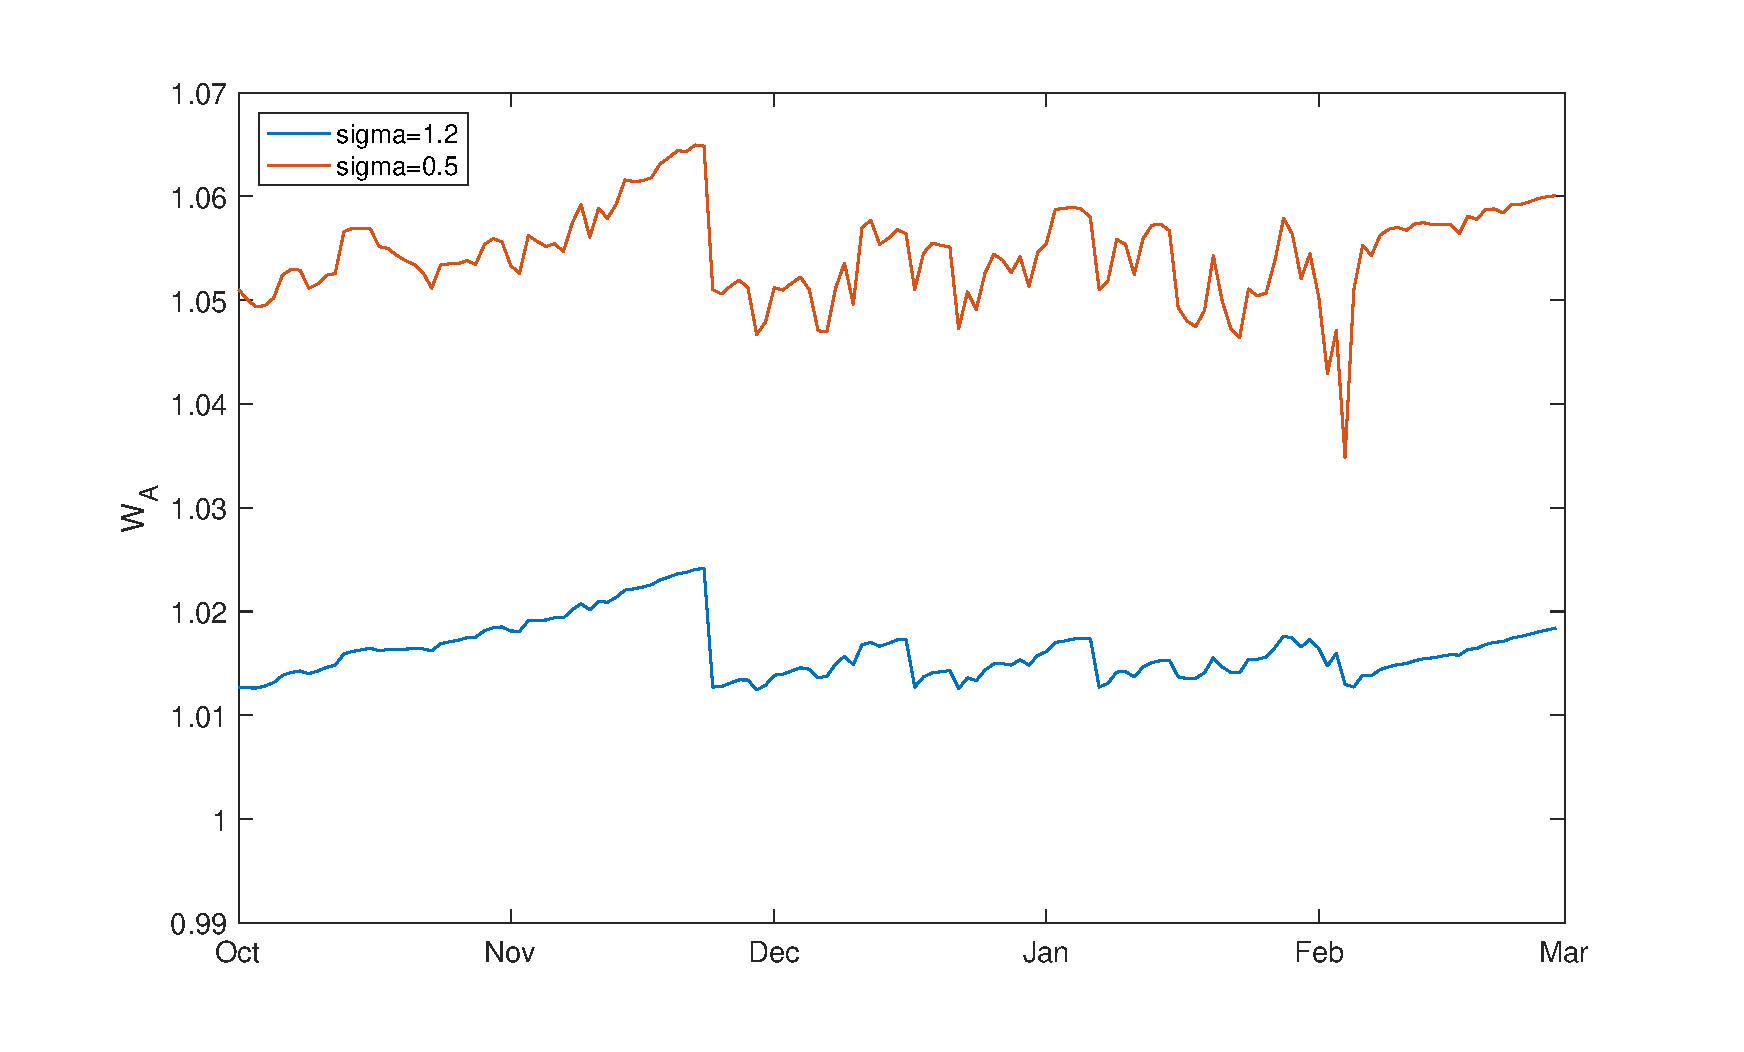
\includegraphics[width=0.9\textwidth]{WA.eps}
\par\end{centering}
\caption{Simulated class A Market Value. $\sigma = 0.0628$ for the blue solid curve, $\sigma=0.0262$ for the red dashed curve. Parameters: $R=0.02\%,\mathcal{H}_{d}=0.25$, $\mathcal{H}_{u} =2$, $T=100$, $r=0.0082\%$ per day ($3\%$ per year). Upward reset takes place on 24 Nov 2017, 17 Dec 2017, and 7 Jan 2018. Downward reset takes place on 5 Feb 2018.}\label{fig:valA}
\end{figure}

Figure \ref{fig:valB} shows the simulated paths from Class B coins. Note that Class B has upward resets (on 24 Nov 2017, 17 Dec 2017, and 7 Jan 2018) with dividend payments \$1.0846, \$1.0467, and \$1.1106 and downward resets on (7 Jan 2018).


\begin{figure}[!htb]
\begin{centering}
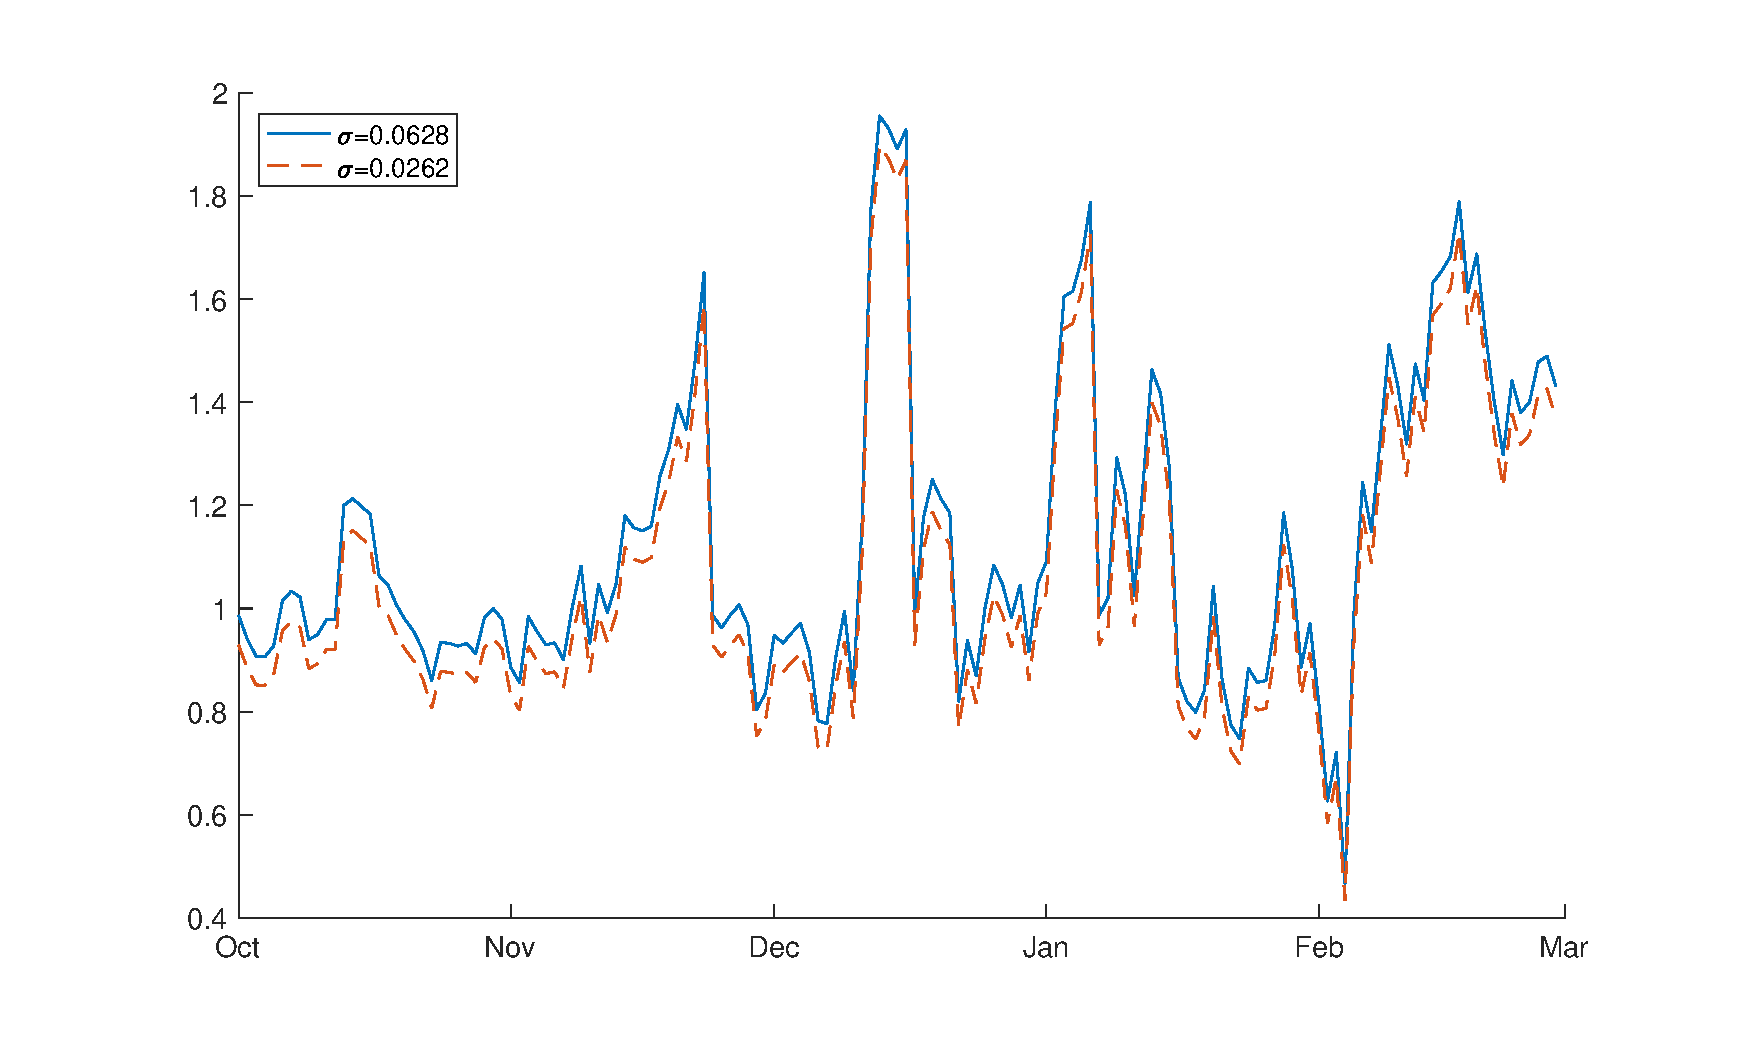
\includegraphics[width=0.9\textwidth]{WB}
\par\end{centering}
\caption{Class B Market Value. $\sigma = 0.0628$ for the blue solid curve, $\sigma=0.0262$ for the red dashed curve. Parameters: $R=0.02\%$, $\mathcal{H}_{d}=0.25$, $\mathcal{H}_{u} =2$, $T=100$, $r=0.0082\%$ per day (3\% per year). Upward reset takes place on 24 Nov 2017, 17 Dec 2017, and 7 Jan 2018. Downward reset takes place on 5 Feb 2018.}
\label{fig:valB}
\end{figure}


\subsection{\texorpdfstring{Market Value of Class \Ap and \Bp}{Lg}}

We can see from Figure \ref{fig:valAPrime} that the market value of Class A$^\prime$ coins is very stable during our sample period, with a value close to 1, except for four downward jumps. These downward jumps correspond to the coupon payment of Class \Ap on the reset dates of Class A. If we de-trend the value of Class \Ap by its net asset value and consider $W_{\Ap}-V_{\Ap}$, it has an annualized standard deviation of $5.4\times 10^{-5}$, which is much smaller than that of $W_{A}-V_{A}$ (0.0178). Even without de-trending, Class \Ap has an annualized return volatility of 0.87\%, which is comparable to that of the short term U.S. treasury bill, 0.96\% (912828K2 Govt, from April 2015 to February 2018).

\begin{figure}[!htb]
\centering
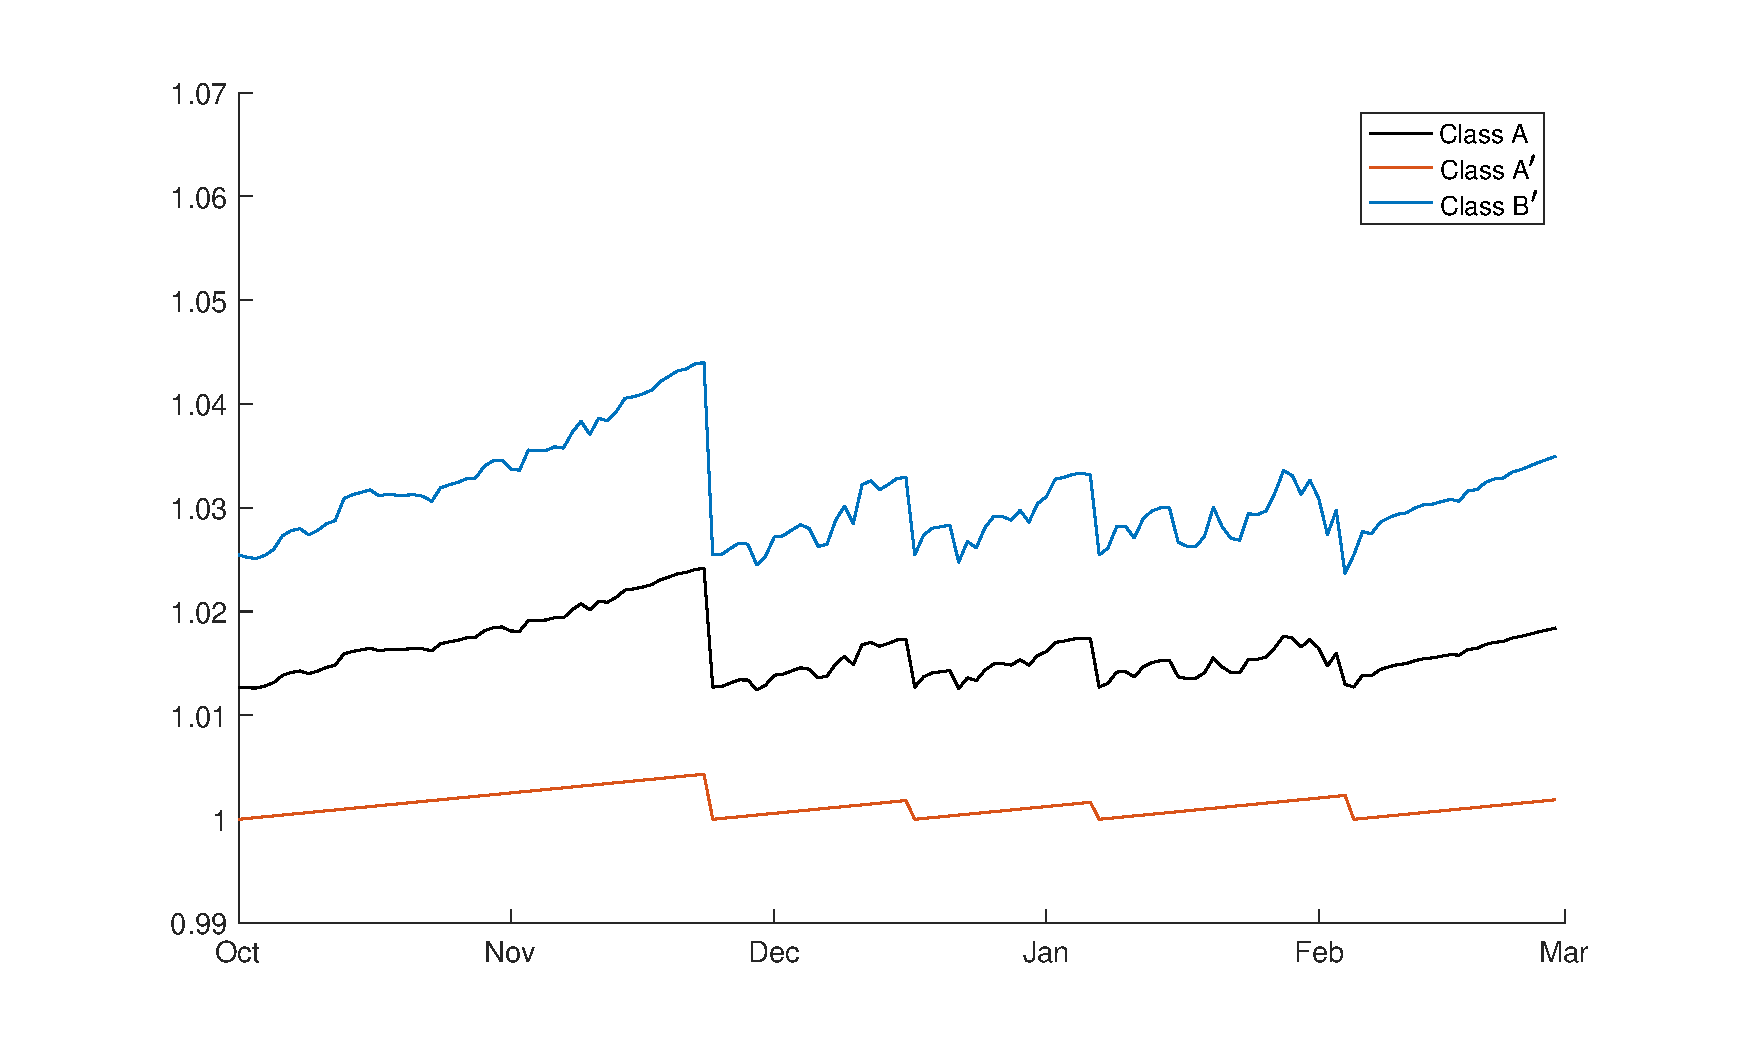
\includegraphics[width=0.9\textwidth]{WABpnoCI4.eps}
\caption{Market Value of Class A$^\prime$ (red) and B$^\prime$ (yellow), compared with Class A (blue). Annualized volatility of Class A$^\prime$ and B$^\prime$ are 0.0087 and 0.0403, respectively. Parameters: $R=0.02\%$ per day, $\mathcal{H}_{d}=0.25$, $\mathcal{H}_{u} =2$, $R^\prime = 0.0082\%$ ($3\%$ per year), $T=100$, $\sigma= 120\%$ per year, $r=0.0082\%$ per day. Upward reset takes place on 24 Nov 2017, 17 Dec 2017, and 7 Jan 2018. Downward reset takes place on 5 Feb 2018.}
\label{fig:valAPrime}
\end{figure}



\subsection{Black Swan Events}
Assume that at time $\eta$, an extreme event happens, and there is a 80\% sudden drop in the ETH price. Assuming $\beta_{\eta-} = 1$, $P_{\eta-} = P_0 = 500$ (so that the relative price $S_{\eta-} = 1$), and $P$ suddenly drops to $P_\eta = 100$. Then the net asset value of Class A coins $V_A^\eta = 2S_{\eta-} \cdot(1-80\%) = 0.4$, while the net asset value of Class \Ap coins is $V^\eta_{\Ap} = 2 \cdot V^\eta_A = 0.8$. A downward reset is triggered, Class A and Class \Ap are fully liquidated, and they receive \$0.4 and \$0.8 payout, respectively. Therefore, when a sudden drop in ETH price occurs, although both Class A and \Ap take a loss, \Ap still recovers a larger value than A.

Now we assume that this kind of downward jump occurs in a jump diffusion model. Specifically,
\begin{align*}
dP_{t}/P_{t-}=r dt+\sigma d\mathcal{B}_{t}+ dJ_t,
\end{align*}
where $J$ is a compound Poisson process with constant intensity 0.2 (per 100 days) and constant jump size $-80\%$. Using simulation based on \eqref{VAL2} and \eqref{VAL3}, we have at time 0, $W_A(0,1) = 0.888$ and $W_{\Ap} (0,1) = 0.962$; in contrast, if there is no jump risk (intensity equals 0), $W_A(0,1) = 1.013$, $W_{\Ap} (0,1) = 1.000$. Therefore, the presence of extreme jump risk has a smaller impact on Class \Ap coins.


\section{Conclusion}
Stable coins, which are cryptocurrencies pegged to other stable financial assets, are desirable for blockchain networks to be used as public accounting ledgers for payment transactions  and as crypto money market accounts for asset allocation involving cryptocurrencies, whereby being often called the ``Holy Grail of cryptocurrency.'' However, existing cryptocurrencies, such as Bitcoins, are too volatile for these purposes. By using option pricing theory, this paper designs, for the first time to our best knowledge, several dual-class structures that offer entitlements to either fixed income stable coins (class A funds) pegged to a traditional currency or leveraged investment opportunities (class B funds). The design is inspired by the dual-purpose funds popular in the U.S. and China. Unlike traditional currencies, the new class A funds record all transactions on a blockchain without centralized counterparties. By using the option pricing theory, we show that the proposed stable coins indeed have very low volatility. Indeed, the class A coin has a volatility comparable to that of the exchange rate of world currencies against U.S. dollar, and the class \Ap coin essentially is pegged to U.S. dollar. When combined with insurance from a government, the design can also serve as a basis for issuing a sovereign cryptocurrency.
%\clearpage


%\bibliographystyle{apalike}
\bibliographystyle{econometrica}
\bibliography{Token1}
%\clearpage


\newpage




%\appendix

%\setcounter{footnote}{0}
%\renewcommand{\thefootnote}{\arabic{footnote}}
%
%\setcounter{equation}{0}
%\setcounter{section}{0}

\setcounter{page}{1}
\renewcommand{\thepage}{A--\arabic{page}}


\begin{appendices}


%\renewcommand{\thesection}{\Roman{section}}

%
%\renewcommand{\thesection}{E\arabic{section}}
%\renewcommand{\theequation}{E--\arabic{equation}}


%\numberwithin{equation}{section}

\begin{center}
{\Large \bf  Online Supplement}

\medskip

{\Large Designing Stable Coins}

\end{center}




%\appendix





\section{Product Design with General Split Ratio}
\label{subsec:General-Product-Design}

% \subsection{General Product Design\label{subsec:General-Product-Design}}

In Section \ref{sec:Product-Design}, we have described a specific product design where Class A is stable relative to USD as target fiat currency and Class B has initial leverage as 2 ($\alpha=1$). In addition, transaction cost in creation and redemption is omitted. In this section, a general case is discussed.

%\subsection{Creation}

Dual-class coins can be created by depositing underlying cryptocurrency to the Custodian contract. Upon receiving underlying cryptocurrency of amount $M_{C}$, the Custodian contract will return to the sender certain amount of Class A and Class B coins. Such amount $C_{A}$ and $C_{B}$ can be calculated by:
\begin{equation}
C_{B}=  \frac{M_{C} P_{0}\beta_t\left(1-c\right)}{1+\alpha},~~~~
C_{A}=  \alpha C_{B},
\label{eq:creation-1}
\end{equation}
where $c$ is the processing fee of the smart contract, $\alpha$ is a positive number to determine the ratio of A and B, and $P_{0}$ is the recorded price of underlying cryptocurrency in target fiat currency at last reset event, and $\beta_t$ is the conversion factor set as 1 at inception and its behaviour is detailed later in Section \ref{subsec:Periodic-Reset} to \ref{subsec:Contingent-Upward-Reset}.

%\subsection{Redemption}

Holders of Class A and Class B coins can withdraw deposited underlying cryptocurrency at any time by performing a redemption. To do this, the user will send $\alpha C$ amount of Class A coins and $C$ amount of Class B coins to the Custodian contract. The contract will deduct Class A and Class B coins, and return to the sender $M_{C}$ underlying cryptocurrency, where $M_{C}$ can be calculated by:
\begin{equation}
M_{C}=\frac{C \left(1-c\right) \left(1+\alpha\right)}{\beta_t P_{0}}.
\label{eq:redemption-1}
\end{equation}

%\subsection{Net Value}

The net value of coins are calculated based on the coupon rate, the elapsed time from last reset event, and the latest underlying cryptocurrency price in target fiat currency fed to the system. In particular:
\begin{equation}
V_{A}^{t}=  1+R\cdot v_t,~~~~
V_{B}^{t}=  \left(1+\alpha\right)\cdot\frac{P_{t}}{\beta_tP_{0}}-\alpha\cdot V_{A}^{t} ,
\label{eq:netvalue-1}
\end{equation}
where $R$ is the daily coupon rate, $v_t$ is the number of days from last reset event, and $P_{t}$ is the current price of underlying cryptocurrency in target fiat currency.
%\subsection{Quantity}
Note that at all time
$
Q_{A}^{t}=\alpha Q_{B}^{t}\ ,
$
where $Q_{A}^{t}$ and $Q_{B}^{t}$ are the total amount of Class A and Class B coins.
%\subsection{Implied Leverage Ratio}
The implied leverage ratio is
\begin{align*}
L_{B}^{t} & =\frac{P_{t}}{\beta_tP_{0}}\cdot\frac{1+\alpha}{V_{B}^{t}}
\end{align*}
Note that at inception or after contingent resets, above simply reduces to $L_{B}^{0}=1+\alpha$.

\subsection{Regular Payout}\label{subsec:Periodic-Reset}

A regular payout is triggered when $v_{t-}=T$. Upon regular payout:
\begin{enumerate}
\item Total amount of both classes coin remain unchanged, $Q_{A}^{t+}=Q_{A}^{t-}$ and $Q_{B}^{t+}=Q_{B}^{t-}$
\item Net asset value of Class A reset to 1 USD
\item Class A holder will receive certain amount of underlying cryptocurrency from the Custodian contract. Such amount for each Class A coin is $U_{A}=\frac{V_{A}^{t}-1}{P_{t}}$
\item Conversion factor $\beta_{t+}=\beta_{t-}\cdot\frac{\left(1+\alpha\right) P_{t}}{\left(1+\alpha\right) P_{t}-\alpha\beta_{t-} P_{0}\left(V_{A}^{t}-1\right)}$
\end{enumerate}
Total value in the system is unchanged after reset:
\begin{align*}
 & U_{A}\cdot P_{t}\cdot Q_{A}^{t-}+Q_{A}^{t+}\cdot V_{A}^{t+}+Q_{B}^{t+}\cdot V_{B}^{t+}\\
= & \left(V_{A}^{t-}-1\right)\cdot Q_{A}^{t-}+Q_{A}^{t-}\cdot1+V_{B}^{t-}\cdot Q_{B}^{t-}\\
= & V_{A}^{t-}\cdot Q_{A}^{t-}+V_{B}^{t-}\cdot Q_{B}^{t-}\ .
\end{align*}



\subsection{Contingent Upward Reset\label{subsec:Contingent-Upward-Reset}}

An upward reset is triggered when $V_{B}^{t}\geqslant\mathcal{H}_{u}$. Upon upward reset:
\begin{enumerate}
\item Total amount of both classes coins remain unchanged, $Q_{A}^{t+}=Q_{A}^{t-}$ and $Q_{B}^{t+}=Q_{B}^{t-}$.
\item Net asset value of both classes reset to 1 target fiat currency.
\item Both classes' holders will receive certain amount of underlying cryptocurrency from the Custodian contract. Such amount for each Class A coin is $U_{A}=\frac{V_{A}^{t}-1}{P_{t}}$ and for each Class B coin is $U_{B}=\frac{V_{B}^{t}-1}{P_{t}}$.
\item Conversion factor $\beta_{t+}$ is reset to $P_t/P_0$.
\end{enumerate}
Total value in the system is unchanged after reset:
\begin{align*}
 & U_{A}\cdot P_{t}\cdot Q_{A}^{t}+U_{B}\cdot P_{t}\cdot Q_{B}^{t}+Q_{A}^{t+}\cdot V_{A}^{t+}+Q_{B}^{t+}\cdot V_{B}^{t+}\\
= & \left(V_{A}^{t}-1\right)\cdot Q_{A}^{t}+\left(V_{B}^{t}-1\right)\cdot Q_{B}^{t}+Q_{A}^{t}\cdot1+Q_{B}^{t}\cdot1\\
= & V_{A}^{t}\cdot Q_{A}^{t}+V_{B}^{t}\cdot Q_{B}^{t}\ .
\end{align*}

\subsection{Contingent Downward Reset\label{subsec:Contingent-Downward-Reset}}

A downward reset is triggered when $V_{B}^{t}\leqslant\mathcal{H}_{d}$. Upon downward reset:
\begin{enumerate}
\item Total amount of Class B coins is reduced to $Q_{B}^{t+}=Q_{B}^{t-}\cdot (V_{B}^{t})^+$.
\item Total amount of Class A coins is reduced to $Q_{A}^{t+}=Q_{B}^{t+}\cdot\alpha$.
\item Net Value of both classes reset to 1 target fiat currency.
\item Class A holders will receive certain amount of underlying cryptocurrency from the Custodian contract. Such amount of each Class A coin is: $D_{A}=\frac{V_{A}^{t}-V_{B}^{t}}{P_{t}}$ if $V_B^t\ge 0$, and $D_{A}=\frac{V_{A}^{t}+V_{B}^{t}/\alpha}{P_{t}}$ if $V_B^t< 0$
\item Conversion factor $\beta_{t+}$ is reset to $P_t/P_0$.
\end{enumerate}
Total value in the system is unchanged after reset:
\begin{align*}
 & D_{A}\cdot P_{t}\cdot Q_{A}^{t-}+Q_{A}^{t+}\cdot V_{A}^{t+}+Q_{B}^{t+}\cdot V_{B}^{t+}\\
= & \left[\left(V_{A}^{t}-V_{B}^{t}\right)\cdot\mathbf{1}_{V_B^t\ge 0}+\left(V_{A}^{t}+V_{B}^{t}/\alpha\right)\cdot\mathbf{1}_{V_B^t< 0}\right]\cdot Q_{A}^{t-}+Q_{B}^{t+}\cdot\alpha\cdot1+Q_{B}^{t+}\cdot1\\
= & V_{A}^{t}\cdot Q_{A}^{t-}-(V_{B}^{t})^+\cdot Q_{B}^{t-}\cdot\alpha-(V_{B}^{t})^-\cdot Q_{B}^{t-}+Q_{B}^{t-}\cdot (V_{B}^{t})^+\cdot\alpha+Q_{B}^{t-}\cdot (V_{B}^{t})^+\\
= & V_{A}^{t}\cdot Q_{A}^{t-}+V_{B}^{t}\cdot Q_{B}^{t-}\ .
\end{align*}
Note above used the fact $Q_{A}^{t-}=Q_{B}^{t-}\cdot\alpha$.



%\subsection{Market Arbitrage}

In the absence of arbitrage, the following price parity shall hold
\[
\alpha\cdot W_{A}^{t}+W_{B}^{t}=\alpha\cdot V_{A}^{t}+V_{B}^{t}\ ,
\]
where $W_{A}^{t}$ is the current price of Class A in target fiat currency, and $W_{B}^{t}$ is the current price of Class B in target fiat currency.

%Along with Equation (\ref{eq:creation-1}), (\ref{eq:redemption-1}) and (\ref{eq:netvalue-1}) in Section \ref{subsec:General-Product-Design}, below should hold:
%\[
%\frac{P_{t}}{P_{0}\cdot\beta}\cdot\left(1-c\right)\leq\frac{\alpha\cdot P_{A}^{t}+P_{B}^{t}}{1+\alpha}\leq\frac{P_{t}}{P_{0}\cdot\beta}\cdot\frac{1}{1-c}\ .
%\]
%On open market, arbitrage opportunity exists when Class A and Class B tokens trade away from their net values and above equation is violated on either side.
%
%\paragraph{Arbitrage via Creation}
%
%When combined market price of Class A and Class B tokens are higher than their combined net values, i.e.
%\[
%\frac{\alpha\cdot P_{A}^{t}+P_{B}^{t}}{1+\alpha}>\frac{P_{t}}{P_{0}\cdot\beta}\cdot\frac{1}{1-c}\ ,
%\]
%arbitrage profit can be exploited by perform DUO token creation:
%\begin{enumerate}
%\item Buy $\frac{1}{1-c}$ underlying tokens from open market for $P_{t}\cdot\frac{1}{1-c}$ target fiat currency equivalent.
%\item Send the underlying tokens to the Custodian contract.
%\item Based on Equation (\ref{eq:creation-1}), receive $P_{0}\cdot\beta\cdot\frac{\alpha}{1+\alpha}$ Class A and $P_{0}\cdot\beta\cdot\frac{1}{1+\alpha}$ Class B tokens.
%\item Sell Class A and Class B tokens on open market for $P_{0}\cdot\frac{\alpha P_{A}^{t}+P_{B}^{t}}{1+\alpha}$ target fiat currency equivalent.
%\end{enumerate}
%The expected payoff of above operations is:
%\[
%P_{0}\cdot\beta\cdot\frac{\alpha P_{A}^{t}+P_{B}^{t}}{1+\alpha}-\frac{P_{t}}{1-c}=P_{0}\cdot\beta\cdot\left(\frac{\alpha\cdot P_{A}^{t}+P_{B}^{t}}{1+\alpha}-\frac{P_{t}}{P_{0}\cdot\beta}\cdot\frac{1}{1-c}\right)>0\ .
%\]
%
%\paragraph{Arbitrage via Redemption}
%
%When combined market price of Class A and Class B tokens are lower than their combined net values, i.e.
%\[
%\frac{P_{t}}{P_{0}\cdot\beta}\cdot\left(1-c\right)>\frac{\alpha\cdot P_{A}^{t}+P_{B}^{t}}{1+\alpha}\ ,
%\]
%similar arbitrage profit can be exploited by perform DUO token redemption:
%\begin{enumerate}
%\item Buy $P_{0}\cdot\beta\cdot\frac{\alpha}{1+\alpha}$ Class A and $P_{0}\cdot\beta\cdot\frac{1}{1+\alpha}$ Class B tokens from open market for $P_{0}\cdot\beta\cdot\frac{\alpha P_{A}^{t}+P_{B}^{t}}{1+\alpha}$ target fiat currency equivalent.
%\item Send Class A and Class B tokens to the Custodian contract.
%\item Based on Equation (\ref{eq:redemption-1}), receive $1-c$ underlying tokens.
%\item Sell underlying tokens on open market for $P_{t}\cdot\left(1-c\right)$ target fiat currency equivalent.
%\end{enumerate}
%The expected payoff of above operations is:
%\[
%P_{t}\cdot\left(1-c\right)-P_{0}\cdot\beta\cdot\frac{\alpha P_{A}^{t}+P_{B}^{t}}{1+\alpha}=P_{0}\cdot\beta\cdot\left(\frac{P_{t}}{P_{0}\cdot\beta}\cdot\left(1-c\right)-\frac{\alpha\cdot P_{A}^{t}+P_{B}^{t}}{1+\alpha}\right)>0\ .
%\]

\section{Derivation of the Pricing Equation}
\label{dpe}
Using contract design under general split ratio $\alpha>0$, similar to \eqref{VAL2}, the value of Class A coins is described by the stochastic representation
\begin{align}
\begin{split}W_{A}(t,S) & =E_{t}\Bigg[e^{-r(T-t)}(RT+W_A(0,S_T-\alpha RT/(1+\alpha)))\cdot\mathbf{1}_{\{T<\tau\land\eta\}}\\
&\quad+e^{-r(\tau-t)}(R\tau+W_{A}(0,1))\cdot\mathbf{1}_{\{\tau\le T\land\eta\}}\\
 & \quad+e^{-r(\eta-t)}(R\eta+1-|V_{B}^{\eta}|+(V_{B}^{\eta})^+W_{A}(0,1))\cdot\mathbf{1}_{\{\eta\le T\land\tau\}}\Bigg].
\end{split}
\label{VAL4}
\end{align}
Note that \eqref{VAL4} becomes \eqref{VAL2} when $\alpha=1$. In this section, under the geometric Brownian motion assumption, we show that \eqref{VAL4} defines a unique bounded function $W_A$, which is exactly the solution to the PDE problem \eqref{eqn:PDEstart} -- \eqref{eqn:PDEend} when $\alpha=1$. We denote $v_s$ and $Y_s$ as the time from last regular payout or reset and the number of A shares at time $s$, respectively. Starting from an initial value 1, $Y$ is reduced by a factor of $\mathcal{H}_d$ on every downward reset dates (thanks to the geometric Brownian motion assumption), reflecting the partial payback of Class A principal. In this remaining of this section, we focus on the right limit process $S_{t+}$, which is still denoted as $S_t$ for simplicity of notations. Further denote $\zeta_i$, $\tau_i$, and $\eta_i$ as the $i$-th regular payout date, upward reset date, and downward reset date after $t$, respectively.
% \footnote{Under the geometric Brownian motion assumption, $S$ and $v$ used in Section \ref{sect:valuation} are left-continuous processes. In this current section, we  }
From the construction of contract, we have
\begin{align*}
dS_t &= rS_tdt+\sigma S_td\mathcal{B}_t,\\
S_{\zeta_i}&=S_{\zeta_i-}-\frac{\alpha}{\alpha+1}Rv_{\zeta_i-},~~ S_{\tau_i}=S_{\eta_i}=1, ~~v_{\tau_i}=v_{\eta_i}=v_{\zeta_i}=0,
\end{align*}
where $\mathcal{B}$ is a Brownian motion under the risk-neutral measure.

First, we derive the following proposition, which expresses the stochastic representation \eqref{VAL4} into a non-recursive form.
\begin{proposition}\label{prop:nonrecur}
	Equation \eqref{VAL4} defines a unique solution $W_A(t,S)$ for $0\le t\le T$, $H_d(t)\le S\le H_u(t)$, which can be written as
	\begin{align}\label{VALnonrecur}
	\begin{split}
	&W_A(t,S)=E_t^{(t,S,1)}\Bigg[\sum_{\zeta_i\ge t}e^{-r(\zeta_i-t)}Y_{\zeta_i-}RT+\sum_{\tau_i\ge t}e^{-r(\tau_i-t)}Y_{\tau_i-}Rv_{\tau_i-}\\
	&\quad+\sum_{\eta_i\ge t}e^{-r(\eta_i-t)}Y_{\eta_i-}(Rv_{\eta_i-}+1-\mathcal{H}_d)\Bigg],
	\end{split}
	\end{align}
	where $E^{(u,s,y)}_t$ is the $\mathbb{Q}$-expectation computed under the initial condition $v_{t-}=u$, $S_{t-}=s$, and $Y_{t-}=y$.\footnote{If $t$ and $S$ are such that $t$ is a regular payout or downward/upward reset date, the right hand side of (\ref{VAL2}) is viewed as the value of the time-$t$ payment plus the expectation with the value of state variables immediately after the jump (if applicable) as time-$t$ starting values.}
\end{proposition}

\begin{proof}[Proof of Proposition \ref{prop:nonrecur}]
	Without loss of generality we prove the case $T=1$. We prove this theorem in three steps.
	{\flushleft\bf Step 1:}
	To see that $W_A$ given by \eqref{VALnonrecur} satisfies \eqref{VAL4}, note that \eqref{VALnonrecur} implies
	\begin{align*}
	\begin{split}
	&W_A(t,S)=E_t^{t,S,1}\Bigg[\sum_{t\le\zeta_i<\tau_1\land\eta_1}e^{-r(\zeta_i-t)}Y_{\zeta_i-}R+e^{-r(\tau_1-t)}Y_{\tau_1-}Rv_{\tau_1-}\cdot\mathbf{1}_{\{\tau_1<\eta_1\}}\\
	&\quad+e^{-r(\eta_1-t)}Y_{\eta_1-}(Rv_{\eta_1-}+1-\mathcal{H}_d)\cdot\mathbf{1}_{\{\eta_1<\tau_1\}}\\
	&\quad+e^{-r(\tau_1\land\eta_1-t)}Y_{\tau_1\land\eta_1}E_{\tau_1\land\eta_1}^{(0,1,Y_{\tau_1\land\eta_1})}\Bigg(\sum_{\xi_i\ge\tau_1\land\eta_1}e^{-r(\zeta_i-\tau_1\land\eta_1)}\frac{Y_{\zeta_i-}}{Y_{\tau_1\land\eta_1}}R\\
	&\quad+\sum_{\tau_i>\tau_1\land\eta_1}e^{-r(\tau_i-\tau_1\land\eta_1)}\frac{Y_{\tau_i-}}{Y_{\tau_1\land\eta_1}}Rv_{\tau_i-}\\
	&\quad+\sum_{\eta_i>\tau_1\land\eta_1}e^{-r(\eta_i-\tau_1\land\eta_1)}\frac{Y_{\eta_i-}}{Y_{\tau_1\land\eta_1}}(Rv_{\eta_i-}+1-\mathcal{H}_d)\Bigg)\Bigg],
	\end{split}
	\end{align*}
	where $E_{\tau_1\land\eta_1}^{(u,s,y)}$ denotes the conditional expectation computed at time $\tau_1\land\eta_1$ with $(v,S,Y)_{\tau_1\land\eta_1}=(u,s,y)$. As a result,
	\begin{align*}
	 &E_{\tau_1\land\eta_1}^{(0,1,Y_{\tau_1\land\eta_1})}\Bigg[\sum_{\xi_i\ge\tau_1\land\eta_1}e^{-r(\zeta_i-\tau_1\land\eta_1)}\frac{Y_{\zeta_i-}}{Y_{\tau_1\land\eta_1}}R+\sum_{\tau_i>\tau_1\land\eta_1}e^{-r(\tau_i-\tau_1\land\eta_1)}\frac{Y_{\tau_i-}}{Y_{\tau_1\land\eta_1}}Rv_{\tau_i-}\\
	&\quad+\sum_{\eta_i>\tau_1\land\eta_1}e^{-r(\eta_i-\tau_1\land\eta_1)}\frac{Y_{\eta_i-}}{Y_{\tau_1\land\eta_1}}(Rv_{\eta_i-}+1-\mathcal{H}_d)\Bigg]\Bigg]\\
	&=E_{0}^{(0,1,1)}\Bigg[\sum_{\xi_i\ge0}e^{-r\zeta_i}Y_{\zeta_i-}R+\sum_{\tau_i\ge0}e^{-r\tau_i}Y_{\tau_i-}Rv_{\tau_i-} \\
	&~ \quad +\sum_{\eta_i\ge0}e^{-r\eta_i}Y_{\eta_i-}(Rv_{\eta_i-}+1-\mathcal{H}_d)\Bigg]\\
	&=W_A(0,1),
	\end{align*}
	where the first equality follows from the Markov property of $(v,S,Y)$ and the fact that time 0 cannot be an interest payment date given $(v,S,Y)_0=(0,1,1)$. Plugging this equation into the previous equation, we get
	\begin{align*}
	&W_A(t,S)=E_t^{(t,S,1)}\Bigg[\sum_{t\le\zeta_i<\tau_1\land\eta_1}e^{-r(\zeta_i-t)}Y_{\zeta_i-}R+e^{-r(\tau_1-t)}Y_{\tau_1-}Rv_{\tau_1-}\cdot\mathbf{1}_{\{\tau_1<\eta_1\}}\\
	&\quad+e^{-r(\eta_1-t)}Y_{\eta_1-}(Rv_{\eta_1-}+1-\mathcal{H}_d)\cdot\mathbf{1}_{\{\eta_1<\tau_1\}}+e^{-r(\tau_1\land\eta_1-t)}Y_{\tau_1\land\eta_1}W_A(0,1)\Bigg]\\
	&=E_t^{(t,S,1)}\Bigg[\sum_{\zeta_i<\tau_1\land\eta_1}e^{-r(i-t)}R+e^{-r(\tau_1-t)}R(\tau_1-\lfloor\tau_1\rfloor+W_A(0,1))\cdot\mathbf{1}_{\{\tau_1<\eta_1\}}\\
	&\quad+e^{-r(\eta_1-t)}(R(\eta_1-\lfloor\eta_1\rfloor)+1-\mathcal{H}_d+\mathcal{H}_d W_A(0,1))\cdot\mathbf{1}_{\{\eta_1<\tau_1\}}\Bigg]
	\end{align*}
	by the definition of $v$, $Y$, and $\zeta$. This yields \eqref{VAL4}.
	
	{\flushleft\bf Step 2:} Next we show that any solution $W_A$ satisfying \eqref{VAL4} is a bounded function of $(t,S)$ in $0\le t\le 1$, $H_d(t)\le S\le H_u(t)$. Indeed,
	\begin{align*}
	&W_A(t,S)=E_t^{(t,S,1)}\Bigg[\sum_{1\le i< \tau\land\eta}e^{-r(i-t)}R+e^{-r(\tau-t)} \Bigg( R(\tau-\lfloor\tau\rfloor)  \\
	&\quad+W_A(0,1))\cdot\mathbf{1}_{\{\tau<\eta\}} \\
	&\quad   +e^{-r(\eta-t)}(R(\eta-\lfloor\eta\rfloor)+1-\mathcal{H}_d+\mathcal{H}_d W_A(0,1) \Bigg) \cdot \mathbf{1}_{\{\eta<\tau\}}\Bigg]\\
	&\le E_t^{(t,S,1)}\Bigg[\sum_{1\le i< \tau\land\eta}e^{-r(i-t)}R   \\
	&\quad +e^{-r(\tau\land\eta-t)}(R+\max\{W_A(0,1),1-\mathcal{H}_d+\mathcal{H}_d W_A(0,1)\})\Bigg]\\
	&\le \frac{e^{-r}R}{1-e^{-r}}+(R+\max\{W_A(0,1),1-\mathcal{H}_d+\mathcal{H}_d W_A(0,1)\}):=\overline{K}.
	\end{align*}
	Note that the right hand side does not depend on $t$ or $S$.
	
	{\flushleft\bf Step 3:} To see the uniqueness, for any $W_A$ satisfying \eqref{VAL4}, by defining the first interest payment time $\theta_1=\tau_1\land\eta_1\land1$, we get
	\begin{align*}
	&W_A(t,S)=E_t^{(t,S,1)}\Bigg[e^{-r(\theta_1-t)}\Bigg((R+W_A(0,S_{\theta_1-}-\alpha R/(1+\alpha)))\cdot\mathbf{1}_{\{\theta_1<\tau_1\land\eta_1\}}\\
	&\quad+(R(\theta_1-\lfloor\theta_1\rfloor)+W_A(0,1))\cdot\mathbf{1}_{\{\theta_1=\tau_1\}}\\
	&\quad+(R(\theta_1-\lfloor\theta_1\rfloor)+1-\mathcal{H}_d+\mathcal{H}_d W_A(0,1))\cdot \mathbf{1}_{\{\theta_1=\eta_1\}}\Bigg)\Bigg]\\
	&=E_t^{(t,S,1)}\Bigg[e^{-r(\theta_1-t)}\Bigg(R\cdot\mathbf{1}_{\{\theta_1=\zeta_1\}}+Rv_{\theta_1-}\cdot\mathbf{1}_{\{\theta_1=\tau_1\}}\\
	&\quad+(Rv_{\theta_1-}+1-\mathcal{H}_d)\cdot \mathbf{1}_{\{\theta_1=\eta_1\}}+Y_{\theta_1} W_A(v_{\theta_1},S_{\theta_1})\Bigg)\Bigg].
	\end{align*}
	Therefore,
	\begin{align*}
	&W_A(t,S) \\
	&=E_t^{(t,S,1)}\Bigg[\Bigg(\sum_{\zeta_i\le\theta_1}e^{-r(\zeta_i-t)}Y_{\zeta_i-}R+\sum_{\tau_i\le\theta_1}e^{-r(\tau_i-t)}Y_{\tau_i-}Rv_{\tau_i-}\\
	&\quad+\sum_{\eta_i\le\theta_1}e^{-r(\eta_i-t)}Y_{\eta_i-}(Rv_{\eta_i-}+1-\mathcal{H}_d)+e^{-r(\theta_1-t)}Y_{\theta_1} W_A(0,S_{\theta_1})\Bigg)\Bigg].
	\end{align*}
	By plugging the expression for $W_A(0,1)$ into the right hand side and using the Markov property, one gets
	\begin{align*}
	&W_A(t,S)=E_t^{(t,S,1)}\Bigg[\Bigg(\sum_{\zeta_i\le\theta_1}e^{-r(\zeta_i-t)}Y_{\zeta_i-}R+\sum_{\tau_i\le\theta_1}e^{-r(\tau_i-t)}Y_{\tau_i-}Rv_{\tau_i-}\\
	&\quad+\sum_{\eta_i\le\theta_1}e^{-r(\eta_i-t)}Y_{\eta_i-}(Rv_{\eta_i-}+1-\mathcal{H}_d)\Bigg)\\
	&\quad+e^{-r(\theta_1-t)}Y_{\theta_1} E_{\theta_1}^{(v_{\theta_1},S_{\theta_1},Y_{\theta_1})}\Bigg[\Bigg(\sum_{\theta_1<\zeta_i\le\theta_2}e^{-r(\zeta_i-\theta_1)}\frac{Y_{\zeta_i-}}{Y_{\eta_i}}R   \\
	&\quad+\sum_{\theta_1<\tau_i\le\theta_2}e^{-r(\tau_i-\theta_1)}\frac{Y_{\tau_i-}}{Y_{\theta_1}}Rv_{\eta_i-}\\
	&\quad+\sum_{\theta_1<\eta_i\le\theta_2}e^{-r(\eta_i-\theta_1)}\frac{Y_{\eta_i-}}{Y_{\theta_1}}(Rv_{\eta_i-}+1-\mathcal{H}_d)+e^{-r(\theta_2-\theta_1)}\frac{Y_{\theta_2}}{Y_{\theta_1}} W_A(v_{\theta_2},S_{\theta_2})\Bigg)\Bigg]\Bigg].
	\end{align*}
	Thus,
	\begin{align*}
	&W_A(t,S) \\
	&=E_t^{(t,S,1)}\Bigg[\Bigg(\sum_{\zeta_i\le\theta_2}e^{-r(\zeta_i-t)}Y_{\zeta_i-}R+\sum_{\tau_i\le\theta_2}e^{-r(\tau_i-t)}Y_{\tau_i-}Rv_{\tau_i-}\\
	&\quad+\sum_{\eta_i\le\theta_2}e^{-r(\eta_i-t)}Y_{\eta_i-}(Rv_{\eta_i-}+1-\mathcal{H}_d)+e^{-r(\theta_2-t)}Y_{\theta_2} W_A(v_{\theta_2},S_{\theta_2})\Bigg)\Bigg].
	\end{align*}
	Repeating this for $N$ times, we get
	\begin{align}\label{eqn:22}
	\begin{split}
	&W_A(t,S)=E_t^{(t,S,1)}\Bigg[\sum_{t\le \zeta_i\le\theta_N}e^{-r(\zeta_i-t)}Y_{\zeta_i-}R+\sum_{t\le \tau_i\le \theta_N}e^{-r(\tau_i-t)}Y_{\tau_i-}Rv_{\tau_i-}\\
	&\quad+\sum_{t\le\eta_i\le \theta_N}e^{-r(\eta_i-t)}Y_{\eta_i-}(Rv_{\eta_i-}+1-\mathcal{H}_d)+e^{-r(\theta_N-t)}Y_{\theta_N}W_A(v_{\theta_N},S_{\theta_N})\Bigg],
	\end{split}
	\end{align}
	where $\theta_N$ denotes the $N$-th interest payment time. Thanks to the boundedness of $W_A$, we have
	\begin{align*}
	0&\le \lim_{N\to\infty}E_t^{(t,S,1)}\left[e^{-r(\theta_N-t)}Y_{\theta_N}W_A(v_{\theta_N},S_{\theta_N})\right] \\
	&\le \overline{K}\cdot\lim_{N\to\infty}E_t^{(t,S,1)}\left[e^{-r(\theta_N-t)}\right]=0.
	\end{align*}
	Here, to see the last equality, it suffices to note that (1) for two consecutive regular payouts $\zeta_i,\zeta_{i+1}$, we have $\zeta_{i+1}-\zeta_{i}\ge T$, therefore $E_t^{t,S,1}\left[e^{-r(\zeta_{i+1}-\zeta_i)}\right]\le e^{-rT}:=K_1<1$; (2) for two consecutive upward resets $\tau_i,\tau_{i+1}$, we have $E_t^{t,S,1}\left[e^{-r(\tau_{i+1}-\tau_i)}\right]=E_0^{0,1,1}\left[e^{-r\tau_1}\right]:=K_2<1$; (3) for two consecutive downward resets $\eta_i,\eta_{i+1}$, we have $E_t^{t,S,1}\left[e^{-r(\eta_{i+1}-\eta_i)}\right]=E_0^{0,1,1}\left[e^{-r\eta_1}\right]:=K_3<1$. Consequently, for $k\ge 1$, we have $$E_t^{t,S,1}\left[e^{-r(\theta_{3k+3}-\theta_{3k})}\right]\le K_1\land K_2\land K_3<1,$$
	since there must be two regular payouts, upward resets or downward resets in $\theta_{3k},\ldots,\theta_{3k+3}$. Therefore,
	\begin{align*}
		E_t^{t,S,1}\left[e^{-r(\theta_{3k+3}-t)}\right]\le e^{rt}\cdot(K_1\land K_2\land K_3)^k\to 0,\text{ as }k\to\infty,
	\end{align*}
	and the claim follows from the monotonicity of $(\theta_k)$. Therefore, by sending $N\to\infty$, we infer that the right hand side of \eqref{eqn:22} converges to \eqref{VALnonrecur}. This shows that any $W_A$ is equal to the right hand side of \eqref{VALnonrecur}, which gives the uniqueness of $W_A$ satisfying \eqref{VAL4}.
\end{proof}


\begin{theorem}\label{thm:main}
$W_{A}$ is the unique classical solution\footnote{By classical solution we mean $W_{A}\in C^{1,2}(Q)\cap C(\overline{Q}\backslash D)$, where $Q=\{(t,S):0\le t<T,H_{d}(t)<S<H_{u}(t)\}$ and $D=\{T\}\times\{H_{d}(T),H_{u}(T)\}$.} to the following partial differential equation on $\{(t,S):0\le t<T,H_{d}(t)<S<H_{u}(t)\}$
\begin{align}
&-\frac{\partial W_{A}}{\partial t}  =\frac{1}{2}\sigma^{2}S^{2}\frac{\partial^{2}W_{A}}{\partial S^{2}}+r S\frac{\partial W_{A}}{\partial S}-r W_{A},&&0\le t<T,H_d(t)<S<H_u(t)\\
&W_{A}(T,S)  =RT+W_{A}(0,S-\frac{\alpha}{1+\alpha}RT),&&H_d(T)<S<H_u(T)\\
&W_{A}(t,H_{u}(t))  =Rt+W_{A}(0,1),&&0\le t\le T\\
&W_{A}(t,H_d(t))  =Rt+1-\mathcal{H}_{d}+\mathcal{H}_{d}W_{A}(0,1),&&0\le t\le T.
\end{align}
\end{theorem}

\begin{proof}[Proof of Theorem \ref{thm:main}]
	Proposition \ref{prop:nonrecur} shows that we can rewrite \eqref{VAL4} in a non-recursive form as
	\begin{align*}
	\begin{split}
	W_A(t,S)&=E_t^{(t,S,1)}\Bigg[\sum_{\zeta_i\ge t}e^{-r(\zeta_i-t)}Y_{\zeta_i-}RT+\sum_{\tau_i\ge t}e^{-r(\tau_i-t)}Y_{\tau_i-}Rv_{\tau_i-}\\
	&\quad+\sum_{\eta_i\ge t}e^{-r(\eta_i-t)}Y_{\eta_i-}(Rv_{\eta_i-}+1-\mathcal{H}_d)\Bigg],
	\end{split}
	\end{align*}
	where $E^{(u,s,y)}_t$ is the $\mathbb{Q}$-expectation computed under the initial condition $v_{t-}=u$, $S_{t-}=s$, and $Y_{t-}=y$. So it remains to show that $W_A$ given as \eqref{VALnonrecur} is the unique classical solution to \eqref{eqn:PDEstart} -- \eqref{eqn:PDEend}. We prove this result based on the stochastic representation result for nonlocal PDE, i.e. Corollary 3.1 in \cite{dai_stochastic_2017}, and in the following we first establish a connection between this theorem and \eqref{prop:nonrecur}.

	We first transform $S_t$ to a process $X_t\in[0,1]$:
	\begin{align*}
		X_t=\Gamma(v_t,S_t)=\frac{S-H_d(v_t)}{H_u(v_t)-H_d(v_t)}.
	\end{align*}
	For $X$, the lower and upper limit becomes 0 and 1, respectively. $X$ can be interpreted as the relative distance of $S$ to the lower limit $H_d$ in $[H_d(t),H_u(t)]$. Under this transform, by Ito's formula, we have
	\begin{align*}
		dX_s=b(v_s,X_s)ds+\sigma(v_s,X_s)d\mathcal{B}_s,
	\end{align*}
	where
	\begin{align*}
		b(v,x)&=r(x-1)-\frac{\alpha}{1+\alpha}\frac{R}{H_u(t)-H_d(t)}+\frac{rH_u(t)}{H_u(t)-H_d(t)},\\
		\sigma(v,x)&=\frac{\sigma H_d(t)}{H_u(t)-H_d(t)}.
	\end{align*}
	Besides, after this transform, the definition $\tau_i$, $\eta_i$ and $\zeta_i$ becomes
	\begin{align*}
		\tau_i&=\inf\{s>\tau_{i-1}:X_{s-}\ge 1\},\eta_i=\inf\{s>\eta_{i-1}:X_{s-}\le 0\}\\
		\zeta_i&=\inf\{s>\zeta_{i-1}:v_{s-}=T,X_{s-}\in(0,1)\}.
	\end{align*}
	On these dates, the change of $X$ is described as
	\begin{align*}
		X_{\zeta_i}&=X_{\zeta_i-}, X_{\tau_i}=X_{\eta_i}=\frac{1-H_d(0)}{H_u(0)-H_d(0)},
	\end{align*}
	and on $\eta_i$, we have
	\begin{align*}
		Y_{\eta_i}=\mathcal{H}_d Y_{\eta_i-},
	\end{align*}
	due to the reduction in the number of shares.

	Now denote $\mathcal{O}=(0,1)$,
	\begin{align*}
		g(x)&=\frac{1-H_d(0)}{H_u(0)-H_d(0)}\cdot\mathbf{1}_{x=0,1}(x)\\
		\tilde{\nu}_{t,x}&=\delta_{0,g(x)}(ds,dz)\\
		\bar{\nu}(t,x)&=\mathcal{H}_d\cdot \mathbf{1}_{x=0}(x)+1_{0<x\le 1}(x)\\
		\theta_i&=\inf\{s>\theta_{i-1}:X_{s-}=0\text{ or }X_{s-}=1\text{ or }v_{s-}=T\}\\
		x&=\Gamma(t,S)\\
		\tilde{W}_A(t,x)&=W_A(t,S).
	\end{align*}
	Also, the payouts of Class A coins at regular payout or reset dates can be expressed as $\tilde{h}(v_{\theta_i-},X_{\theta_i-},\bar{\nu}(X_{\theta_i-})$, where
	$\tilde{h}(v,x,u)=1-u+Rv.$
	Using the above definitions, $W_A$ defined in \eqref{VALnonrecur} can be expressed as
	\begin{align*}
		\tilde{W}_A(t,x)=E_t^x\left[\sum_{\theta_i\ge t}e^{-r(\theta_i-t)}Y_{\theta_i-}\tilde{h}(v_{\theta_i-},X_{\theta_i-},\bar{\nu}(X_{\theta_i-}))\right].
	\end{align*}
	where $E_t^x$ means the expectation calculated under $X_{t-}=x$, $v_{t-}=t$ and $Y_{t-}=1$. Then, Corollary 3.1 in \cite{dai_stochastic_2017} shows that $\tilde{W}_A$ is the unique classic solution to
	\begin{align}\label{eqn:transformedPDEstart}
		-\der{\tilde{W}_A}{t}&-\frac{1}{2}\sigma^2(t,x)\dder{\tilde{W}_A}{x}-b(t,x)\der{\tilde{W}_A}{x}=0 && \text{ in }[0,T)\times(0,1)\\
		\tilde{W}_A(T,x)&=RT+\tilde{W}_A(0,g(x)) && \text{ in }(0,1)\\
		\tilde{W}_A(t,0)&=1-\bar{\nu}(0)+Rt+\bar{\nu}(0)\tilde{W}_A(0,g(0)) && \text{ on }[0,T]\\ \label{eqn:transformedPDEend}
		\tilde{W}_A(t,1)&=Rt+\tilde{W}_A(0,g(1)) && \text{ on }[0,T].
	\end{align}
	By reverting the transform $(t,s)\mapsto(t,x)=\left(t,\frac{s-H_d(t)}{H_u(t)-H_d(t)}\right)$, we conclude that $W_A$ defined in \eqref{VAL4} is the unique classical solution to \eqref{eqn:PDEstart} -- \eqref{eqn:PDEend}.
\end{proof}

\section{Numerical Procedure for the Pricing Equation}\label{subsec:Numerical-Procedure-for}

We propose an iterative algorithm to obtain a numerical solution of the periodic parabolic terminal-boundary value problem ($\ref{eqn:PDEstart}$) \textendash{} ($\ref{eqn:PDEend}$).

\begin{center}
Algorithm 1
\end{center}

1. Set the initial guess $W_{A}^{(0)}=0$.

2.  For $i=1,2,\cdots$: Given $W_{A}^{(i-1)}$, solve for $W_{A}^{(i)}$, the solution to the equation
\begin{align*}
-\frac{\partial W_{A}}{\partial t}= & \frac{1}{2}\sigma^{2}S^{2}\frac{\partial^{2}W_{A}}{\partial S^{2}}+r S\frac{\partial W_{A}}{\partial S}-r W_{A} &  & 0\le t<T,H_{d}(t)<S<H_{u}(t)\\
W_{A}(1,S)= & RT+W_{A}^{(i-1)}(0,S-\frac{1}{2}RT) &  & H_{d}(t)<S<H_{u}(t)\\
W_{A}(t,H_{u}(t))= & Rt+W_{A}^{(i-1)}(0,1) &  & 0\le t\le T\\
W_{A}(t,H_{d}(t))= & Rt+1-\mathcal{H}_{d}+\mathcal{H}_{d}W_{A}^{(i-1)}(0,1) &  & 0\le t\le T.
\end{align*}


3.  If $||W_{A}^{(i)}-W_{A}^{(i-1)}||<$ tolerance, stop and return $W_{A}^{(i)}$; otherwise set $i=i+1$ and go to step 2.

The following theorem ensures the convergence of Algorithm 1.

\begin{theorem}\label{thm:convergence}
	The sequence $(W_A^{(k)})_{k\ge 1}$ defined in Algorithm 1 is monotonically increasing, and it converges to $W_A$ uniformly.
\end{theorem}
\begin{proof}[Proof of Theorem \ref{thm:convergence}]
	We follow the notations in Section \ref{dpe}. From the proof of Theorem \ref{thm:main}, it suffices to consider the sequence $(\tilde{W}_A^{(k)})$ defined via the transformed equation \eqref{eqn:transformedPDEstart} -- \eqref{eqn:transformedPDEend} by iteration with $\tilde{W}_A^{(0)}=0$. Indeed, once we show that $(\tilde{W}_A^{(k)})$ converges uniformly to $\tilde{W}_A$, by reverting the transform $(t,s)\mapsto(t,x)=\left(t,\frac{s-H_d(t)}{H_u(t)-H_d(t)}\right)$, we have that $(W_{A}^{(k)})$ also converges uniformly to $W_A$, which establishes the theorem. We shall do it in the following two steps.

	{\bf Step I.} First, we show that the solution $\tilde{W}_A^{(k)}(t,x)$ can be stochastically represented as
	\begin{align*}
		\tilde{W}_A^{(k)}(t,x)=E_t^x\left[\sum_{t\le \theta_i\le \theta_k}e^{-r(\theta_i-t)}Y_{\theta_i-}\tilde{h}(v_{\theta_i-},X_{\theta_i-},\bar{\nu}(X_{\theta_i-}))\right].
	\end{align*}
	Indeed, for $k=1$, by Feynman-Kac representation for diffusion processes, the equation
	\begin{align*}
	-\frac{\partial \tilde{W}_{A}}{\partial t}= & \frac{1}{2}\sigma^{2}(t,x)\frac{\partial^{2}\tilde{W}_{A}}{\partial x^{2}}+b(t,x)\frac{\partial \tilde{W}_{A}}{\partial x}-r \tilde{W}_{A} &  & 0\le t<T,0<x<1\\
	\tilde{W}_{A}(T,x)= & RT &  & 0<x<1\\
	\tilde{W}_{A}(t,1)= & Rt&  & 0\le t\le T\\
	\tilde{W}_{A}(t,0)= & Rt+1-\mathcal{H}_{d} &  & 0\le t\le T.
	\end{align*}
	has a unique classical solution $\tilde{W}_A^{(1)}\in C^{1,2}(Q)\cap C(\overline{Q}\backslash D)$, which can be represented as
	\begin{align*}
		\tilde{W}_A^{(1)}(t,x)=E_t^x\left[e^{-r(\theta_1-t)}Y_{\theta_1-}\tilde{h}(v_{\theta_1-},X_{\theta_1-},\bar{\nu}(X_{\theta_1-}))\right].
	\end{align*}
	This establishes the claim for $k=1$. Now assume that this claim has been established for $k=i$, $i>1$. Then we have
	\begin{align*}
		&E_t^x\left[\sum_{t\le \theta_j\le \theta_{i+1}}e^{-r(\theta_j-t)}Y_{\theta_j-}\tilde{h}(v_{\theta_j-},X_{\theta_j-},\bar{\nu}(X_{\theta_j-}))\right]\\
		% &=E_t^x\left[e^{-r(\theta_{1}-t)}Y_{\theta_{1}-}\tilde{h}(v_{\theta_{1}-},X_{\theta_{1}-},\bar{\nu}(X_{\theta_{1}-}))\right]\\
		% &\quad+E_t^x\left[\sum_{\theta_1< \theta_j\le \theta_{i+1} }e^{-r(\theta_j-t)}Y_{\theta_j-}\tilde{h}(v_{\theta_j-},X_{\theta_j-},\bar{\nu}(X_{\theta_j-}))\right]\\
		&=E_t^x\left[e^{-r(\theta_{1}-t)}Y_{\theta_{1}-}\tilde{h}(v_{\theta_{1}-},X_{\theta_{1}-},\bar{\nu}(X_{\theta_{1}-}))\right]\\
		&\quad+E_t^x\left[e^{-r(\theta_1-t)}E_{\theta_1}^{v_{\theta_1},X_{\theta_1},Y_{\theta_1}}\left[\sum_{\theta_1< \theta_j\le \theta_{i+1} }e^{-r(\theta_j-\theta_1)}Y_{\theta_j-}\tilde{h}(v_{\theta_j-},X_{\theta_j-},\bar{\nu}(X_{\theta_j-}))\right]\right]\\
		&=E_t^x\left[e^{-r(\theta_{1}-t)}Y_{\theta_{1}-}\tilde{h}(v_{\theta_{1}-},X_{\theta_{1}-},\bar{\nu}(X_{\theta_{1}-}))+e^{-r(\theta_1-t)}Y_{\theta_1}\tilde{W}_A^{(i)}(v_{\theta_1},X_{\theta_1})\right],
	\end{align*}
	where the last equality is from the Markov property and time-homogeneity of $(v,X,Y)$. On the other hand, from the Feynman-Kac representation, the equation
	\begin{align*}
	-\frac{\partial \tilde{W}_{A}}{\partial t}= & \frac{1}{2}\sigma^{2}(t,x)\frac{\partial^{2}\tilde{W}_{A}}{\partial x^{2}}+b(t,x)\frac{\partial \tilde{W}_{A}}{\partial x}-r \tilde{W}_{A} &  & 0\le t<T,0<x<1\\
	\tilde{W}_{A}(T,x)= & RT+\tilde{W}_{A}^{(i)}(0,g(x)) &  & 0<x<1\\
	\tilde{W}_{A}(t,1)= & Rt+\tilde{W}_{A}^{(i)}(0,g(1)) &  & 0\le t\le T\\
	\tilde{W}_{A}(t,0)= & Rt+1-\mathcal{H}_{d}+\mathcal{H}_{d}\tilde{W}_{A}^{(i)}(0,g(0)) &  & 0\le t\le T.
	\end{align*}
	has a unique classical solution, $\tilde{W}_A^{(i+1)}$, which can be represented as
	\begin{align*}
		\tilde{W}_A^{(i+1)}(t,x)&=E_t^x\Bigg[e^{-r(\theta_{1}-t)}Y_{\theta_{1}-}\tilde{h}(v_{\theta_{1}-},X_{\theta_{1}-},\bar{\nu}(X_{\theta_{1}-}))\\
		&\quad+e^{-r(\theta_1-t)}Y_{\theta_1}\tilde{W}_A^{(i)}(v_{\theta_1},X_{\theta_1})\Bigg].
	\end{align*}
	Therefore,
	\begin{align*}
		\tilde{W}_A^{(i+1)}(t,x)=E_t^x\left[\sum_{t\le \theta_j\le \theta_{i+1}}e^{-r(\theta_j-t)}Y_{\theta_j-}\tilde{h}(v_{\theta_j-},X_{\theta_j-},\bar{\nu}(X_{\theta_j-}))\right],
	\end{align*}
	and the claim is proved by induction.

	{\bf Step II.} Next we prove the uniform convergence of $(\tilde{W}_A^{(k)})$ to $\tilde{W}_A$. To see this,
	\begin{align*}
		&|\tilde{W}_A^{(k)}(t,x)-\tilde{W}_A(t,x)|\\
		&=\left|E_t^x\left[e^{-r(\theta_k-t)}\sum_{\theta_j> \theta_{k}}e^{-r(\theta_j-\theta_k)}Y_{\theta_j-}\tilde{h}(v_{\theta_j-},X_{\theta_j-},\bar{\nu}(X_{\theta_j-}))\right]\right|\\
		&\le \bar{K}\cdot \sup_{(t,x)\in[0,T)\times(0,1)}E_t^x\left[e^{-r(\theta_k-t)}\right],
	\end{align*}
	where $\bar{K}$ is as defined in the proof of Proposition \ref{prop:nonrecur}.

	We claim that the right hand side converges to 0. Suppose this claim is proved, we then have the uniform convergence of $(\tilde{W}_A^{(k)})$ in $[0,T)\times(0,1)$. Using the terminal and boundary conditions of the equation for $\tilde{W}_A^{(k)}$,  $(\tilde{W}_A^{(k)})$ also converges uniformly on $[0,T]\times[0,1]$.

	To verify the claim, it suffices to note that (1) for two consecutive regular payouts $\zeta_i,\zeta_{i+1}$, we have $\zeta_{i+1}-\zeta_{i}\ge T$, therefore $E_t^x\left[e^{-r(\zeta_{i+1}-\zeta_i)}\right]\le e^{-rT}:=K_1<1$; (2) for two consecutive upward resets $\tau_i,\tau_{i+1}$, we have $E_t^x\left[e^{-r(\tau_{i+1}-\tau_i)}\right]=E_0^{g(1)}\left[e^{-r\tau_1}\right]:=K_2<1$; (3) for two consecutive downward resets $\eta_i,\eta_{i+1}$, we have $E_t^x\left[e^{-r(\eta_{i+1}-\eta_i)}\right]=E_0^{g(0)}\left[e^{-r\eta_1}\right]:=K_3<1$. Consequently, for $k\ge 1$, we have $$E_t^x\left[e^{-r(\theta_{3k+3}-\theta_{3k})}\right]\le K_1\land K_2\land K_3<1,$$
	since there must be two consecutive regular payouts, upward resets or downward resets in $\theta_{3k},\ldots,\theta_{3k+3}$. Therefore,
	\begin{align*}
		\sup_{(t,x)\in[0,T)\times(0,1)} E_t^x\left[e^{-r(\theta_{3k+3}-t)}\right]\le e^{rt}\cdot(K_1\land K_2\land K_3)^k\to 0,\text{ as }k\to\infty,
	\end{align*}
	and the claim follows from the monotonicity of $(\theta_k)$.
\end{proof}


\section{Class A0 and A1 Coins}\label{sect:A0}

In this extension, each Class A coin is split into one Class A0 coin and one Class A1 coin. On the next coupon payment date or reset date $t$, Class A1 receives the coupon payment for Class A, and then Class A1 is terminated. Class A0 is then split into Class A0 coin and Class A1 coin, until the next reset when Class A1 receives payment and A0 is split again, so on and so forth. At any time, the quantity of Class A0 and A1 maintains 1:1. At any time, the value of Class A1 equals the expected discounted value of Class A's next payment on the next reset or coupon payment date. The value of Class A0 equals the difference between values of Class A and A1. Using the same example as in Section \ref{subsect:vanilla}, Figure \ref{fig:A0} illustrates the cash flow of Class A0 and A1 coins.

\begin{figure}[p]
\centering
	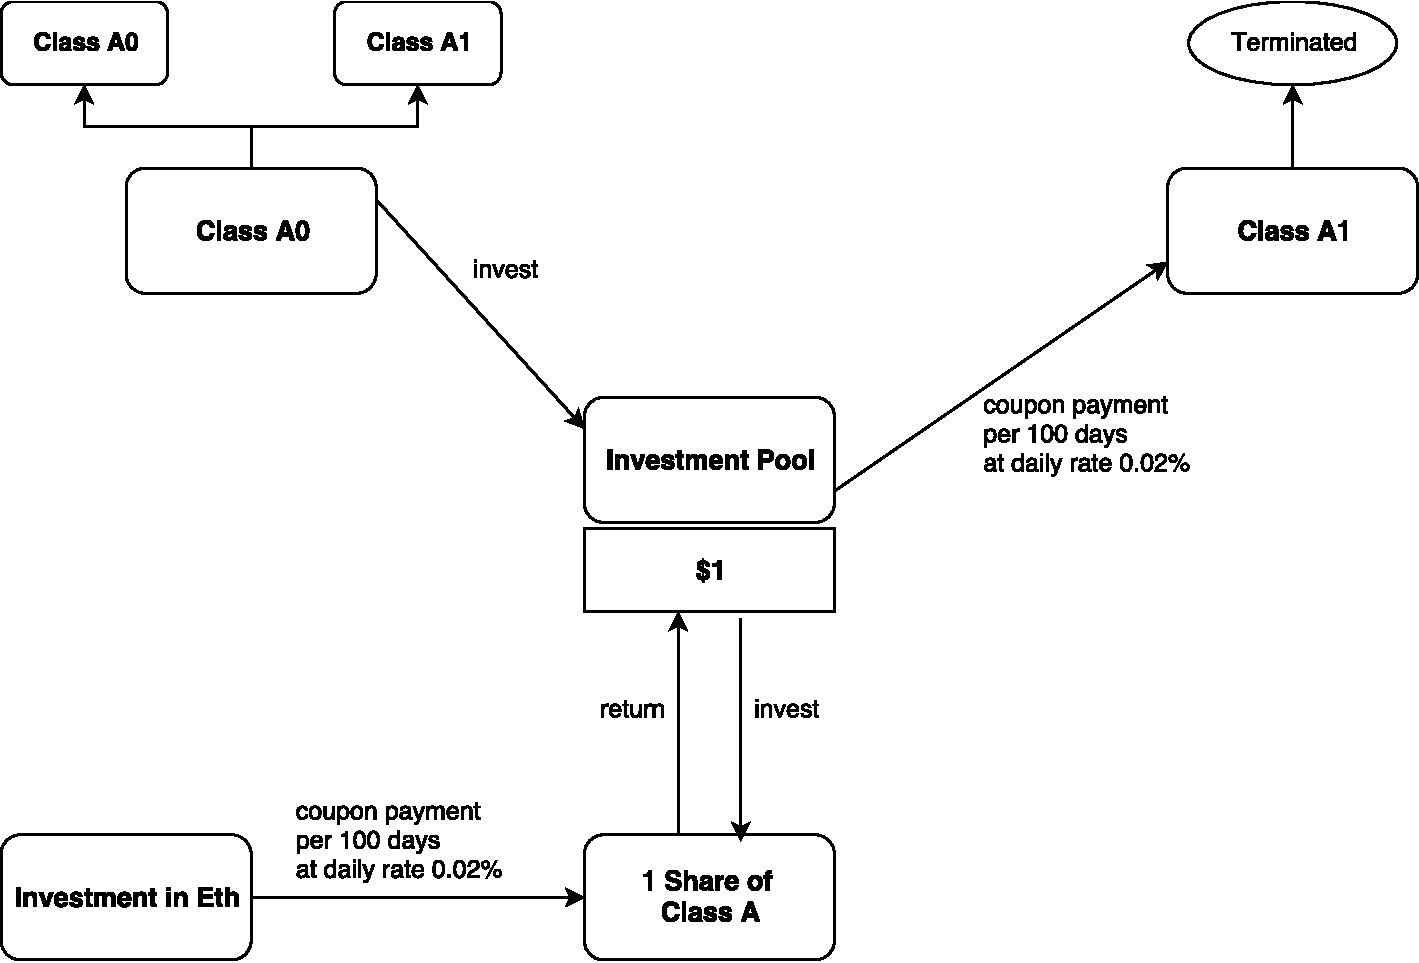
\includegraphics[width=0.58\textwidth]{A0_periodic}
	\vspace{1em}
	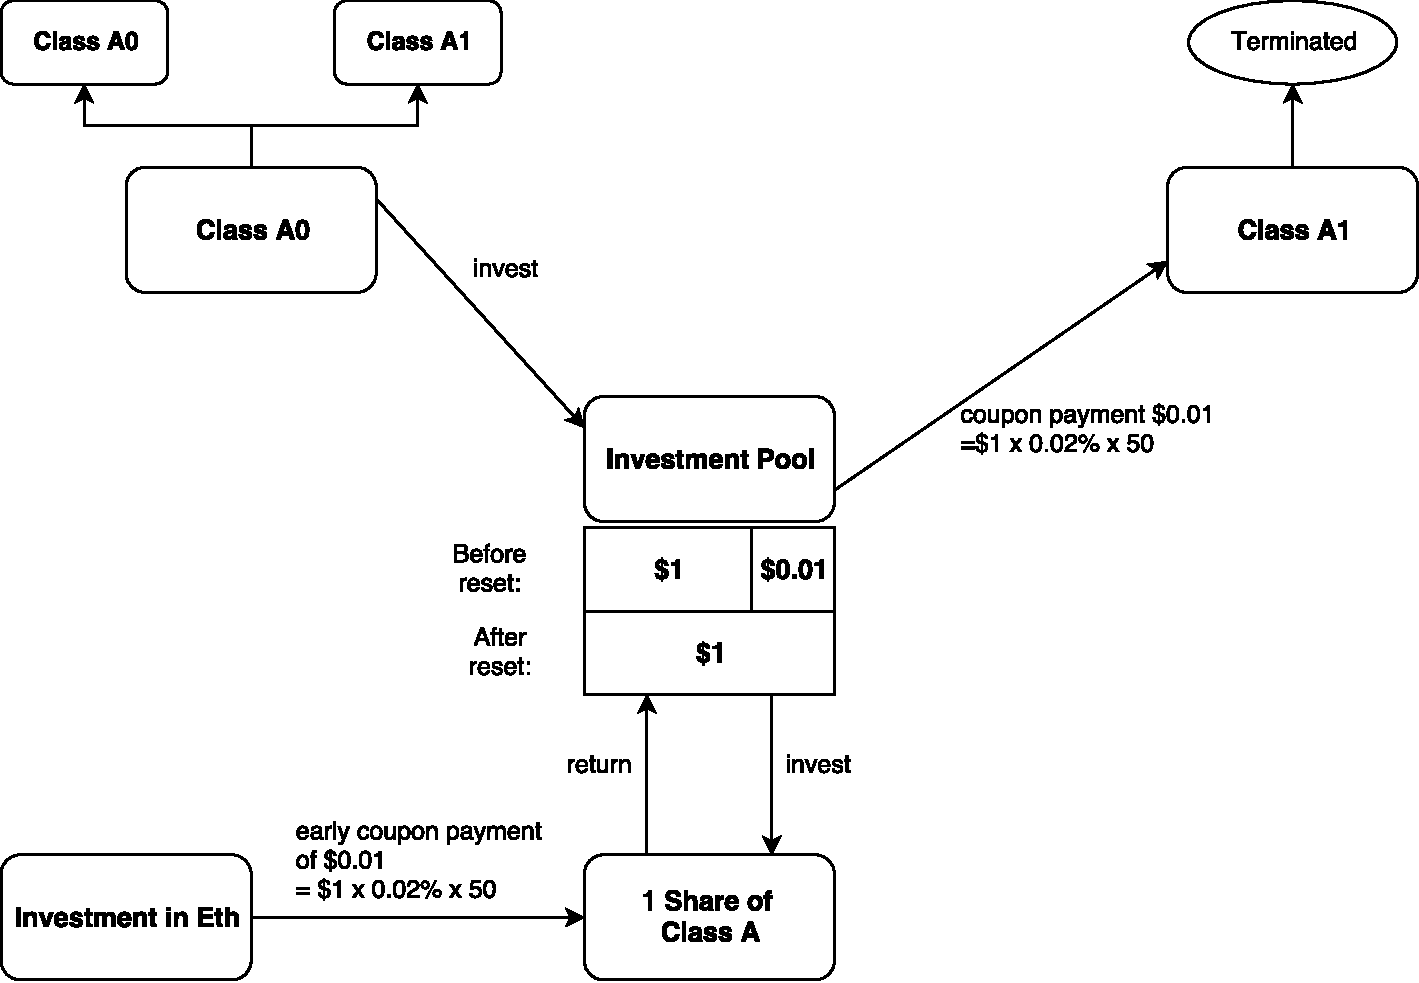
\includegraphics[width=0.58\textwidth]{A0_upward}
	\vspace{1em}
	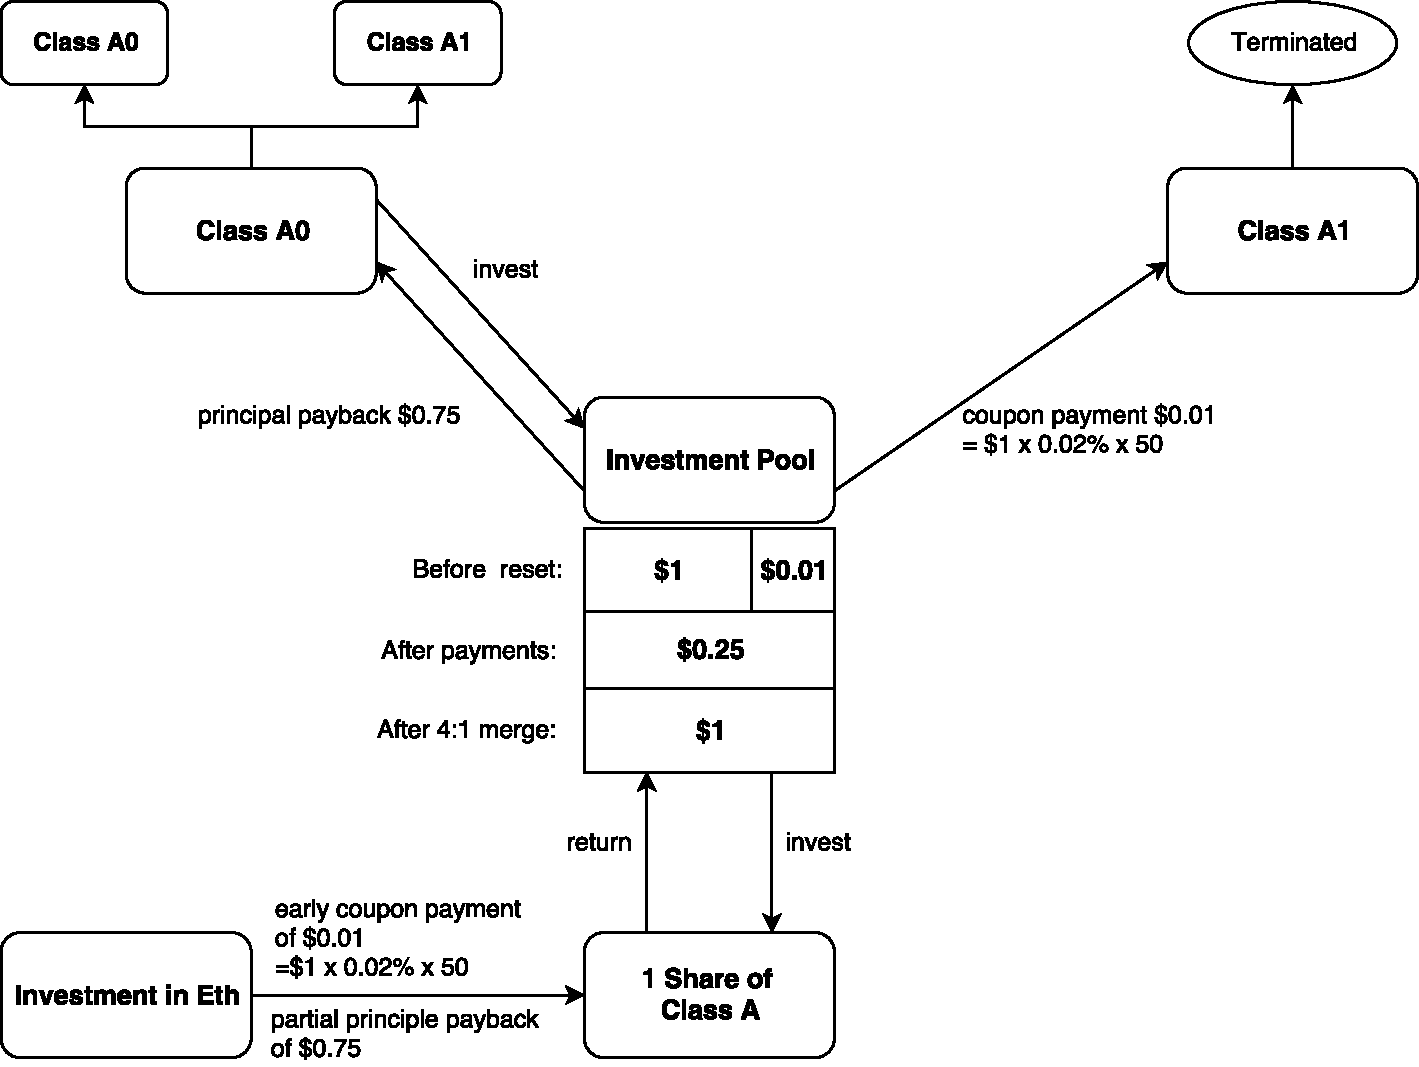
\includegraphics[width=0.58\textwidth]{A0_downward}
	\caption{{\bf Top Figure:} Class A0 receives no coupon.  Class A1 receives all the coupon payment. After the coupon payment, Class A1 is terminated, and 1 Class A0 is split into 1 new Class A0 and Class A1. {\bf Middle Figure:} Upward Reset of Class A0. After 50 days, Class B's net asset value grows to \$2, triggering an upward reset. {\bf Bottom Figure:} After another 50 days, Class B's net asset value drops to \$0.25, triggering a downward reset. }\label{fig:A0}
\end{figure}

By contract design, the coupon of Class A1 is delivered in the form of the underlying cryptocurrency, whose value in USD may subject to volatile changes due to the high volatility of ETH. In contrast, the coupon of Class A0 is paid in the form of Class A1 coins, whose value in USD is much less volatile compared to ETH. Therefore, Class A0 is more suitable for investors with lower risk tolerance or are less active on the market; upon receiving Class A1 coins as coupon, they have a relatively longer period of time to liquidate the coins before its value changes noticeably. In contrast, Class A1 is more suitable for investors who are willing to take certain degree of risk and are more active on the market; so that upon receiving the underlying cryptocurrency, they can monitor the market actively and spot a good opportunity to liquidate the underlying cryptocurency.


Under the risk-neutral pricing framework, the market value $W_{A1}(t,S)$ of Class A1 coin is given as
\begin{align*}
 & E_{t}\Bigg[e^{-r(\zeta-t)}RT\cdot\mathbf{1}_{\{\zeta\le\tau,\eta\}}+e^{-r(\tau-t)}R\tau\cdot\mathbf{1}_{\{\tau<\eta,\zeta\}}\\
 &\quad+e^{-r(\eta-t)}(R\eta-(V_B^{\eta})^-)^+\cdot\mathbf{1}_{\{\eta<\tau,\zeta\}}\Bigg],
\end{align*}
where the first regular payout time $\zeta$, the first upward reset time $\tau$ and the first downward reset time $\eta$ are defined as before. On a downward reset, if $V_B^{\eta}>0$, A1 gets the coupon payment $R\eta$; if $V_B^{\eta}\le 0$, A1 only gets a part of the coupon $(R\eta+V_B^{\eta})^+ < R\eta$.

By assuming that $P_t$ follows a geometric Brownian motion, $W_{A1}$ is the unique solution of the following PDE
\begin{align*}
&-\frac{\partial W_{A1}}{\partial t}  =\frac{1}{2}\sigma^{2}S^{2}\frac{\partial^{2}W_{A1}}{\partial S^{2}}+r S\frac{\partial W_{A1}}{\partial S}-r W_{A1},&&0\le t<T, H_d(t)<S<H_u(t)\\
&W_{A1}(T,S)  =RT,&&H_d(T)<S<H_u(T)\\
&W_{A1}(t,H_{u}(t))  =Rt,&&0\le t\le T\\
&W_{A1}(t,H_d(t))  =Rt,&&0\le t\le T.
\end{align*}
Finally, the value of Class A0 coin is calculated as $W_{A0}=W_A-W_{A1}$.


\begin{figure}[!htb]
\centering
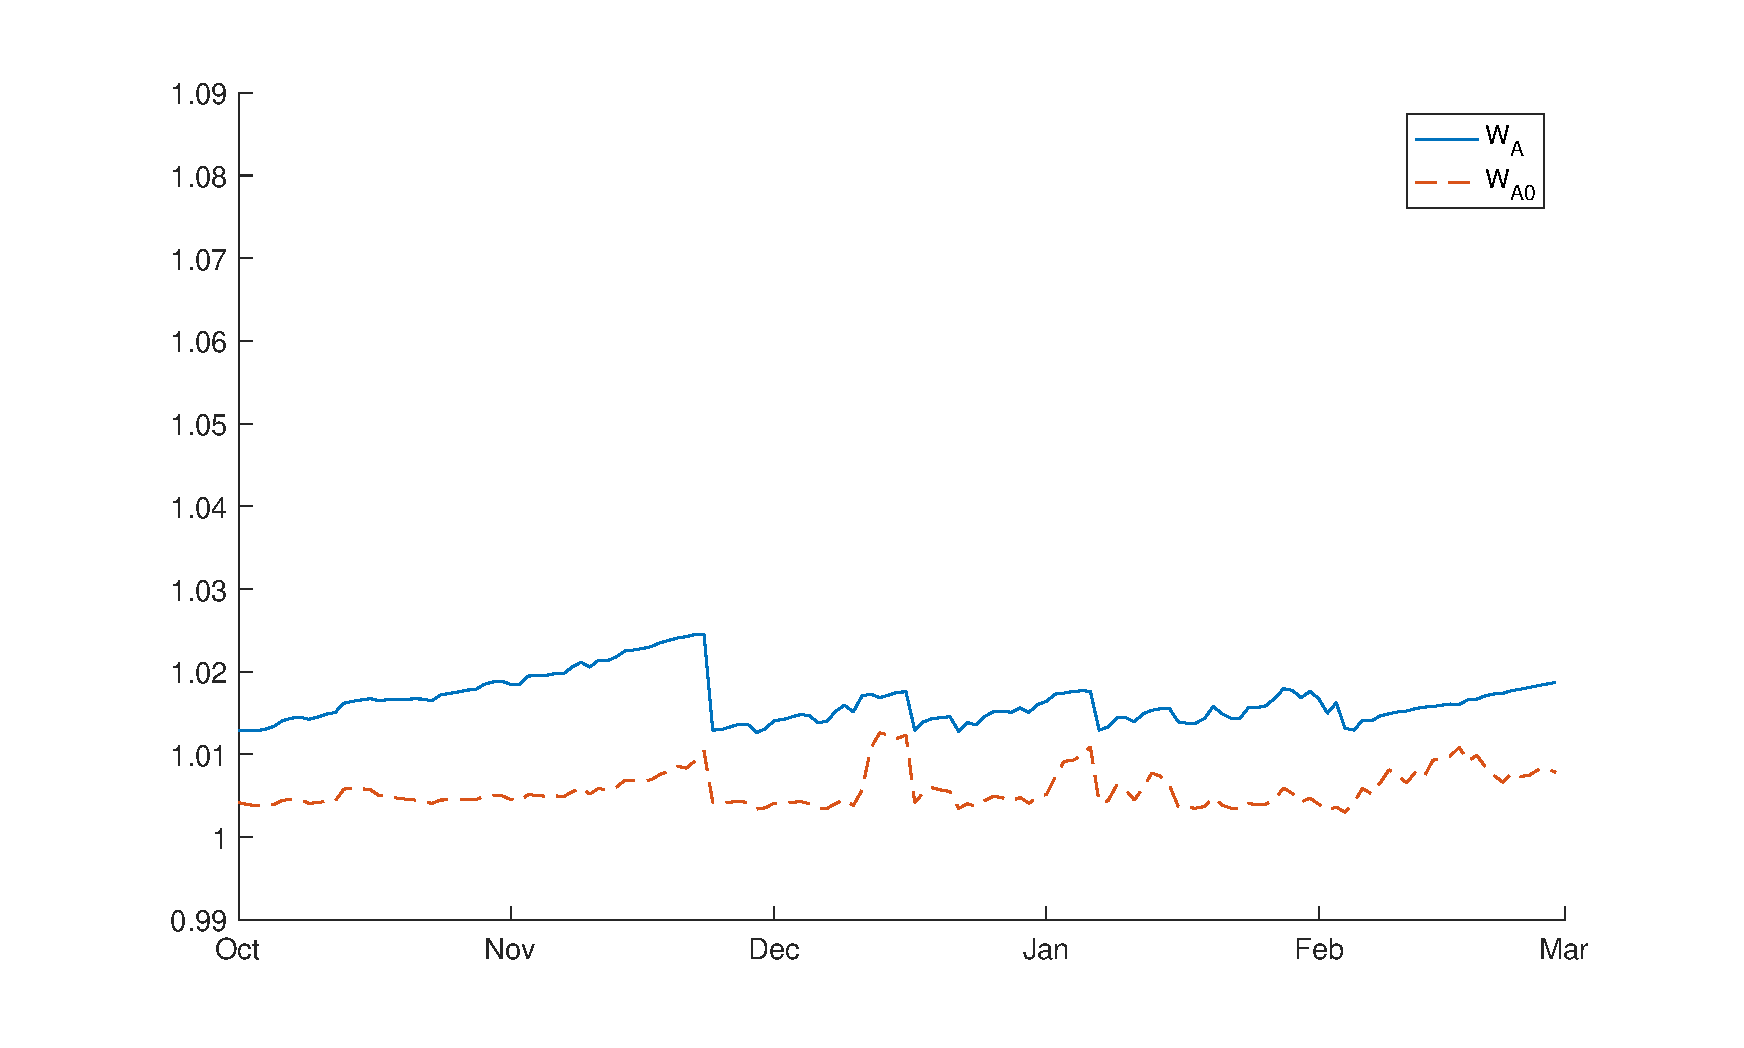
\includegraphics[width=0.9\textwidth]{WA0_alpha1.eps}
\caption{Market Value of Class A0 compared to Class A. Annualized volatility of Class A0 is 0.0254. Parameters: $R=0.02\%,\mathcal{H}_{d}=0.25,\mathcal{H}_{u} =2,T=100,\sigma= 120 \% \text{ per year}, r=0.0082\%$ (3\% per year). Upward reset takes place on 24 Nov 2017, 17 Dec 2017, and 7 Jan 2018. Downward reset takes place on 5 Feb 2018.}
\label{fig:valA0a1}
\end{figure}


\begin{figure}[!htb]
\centering
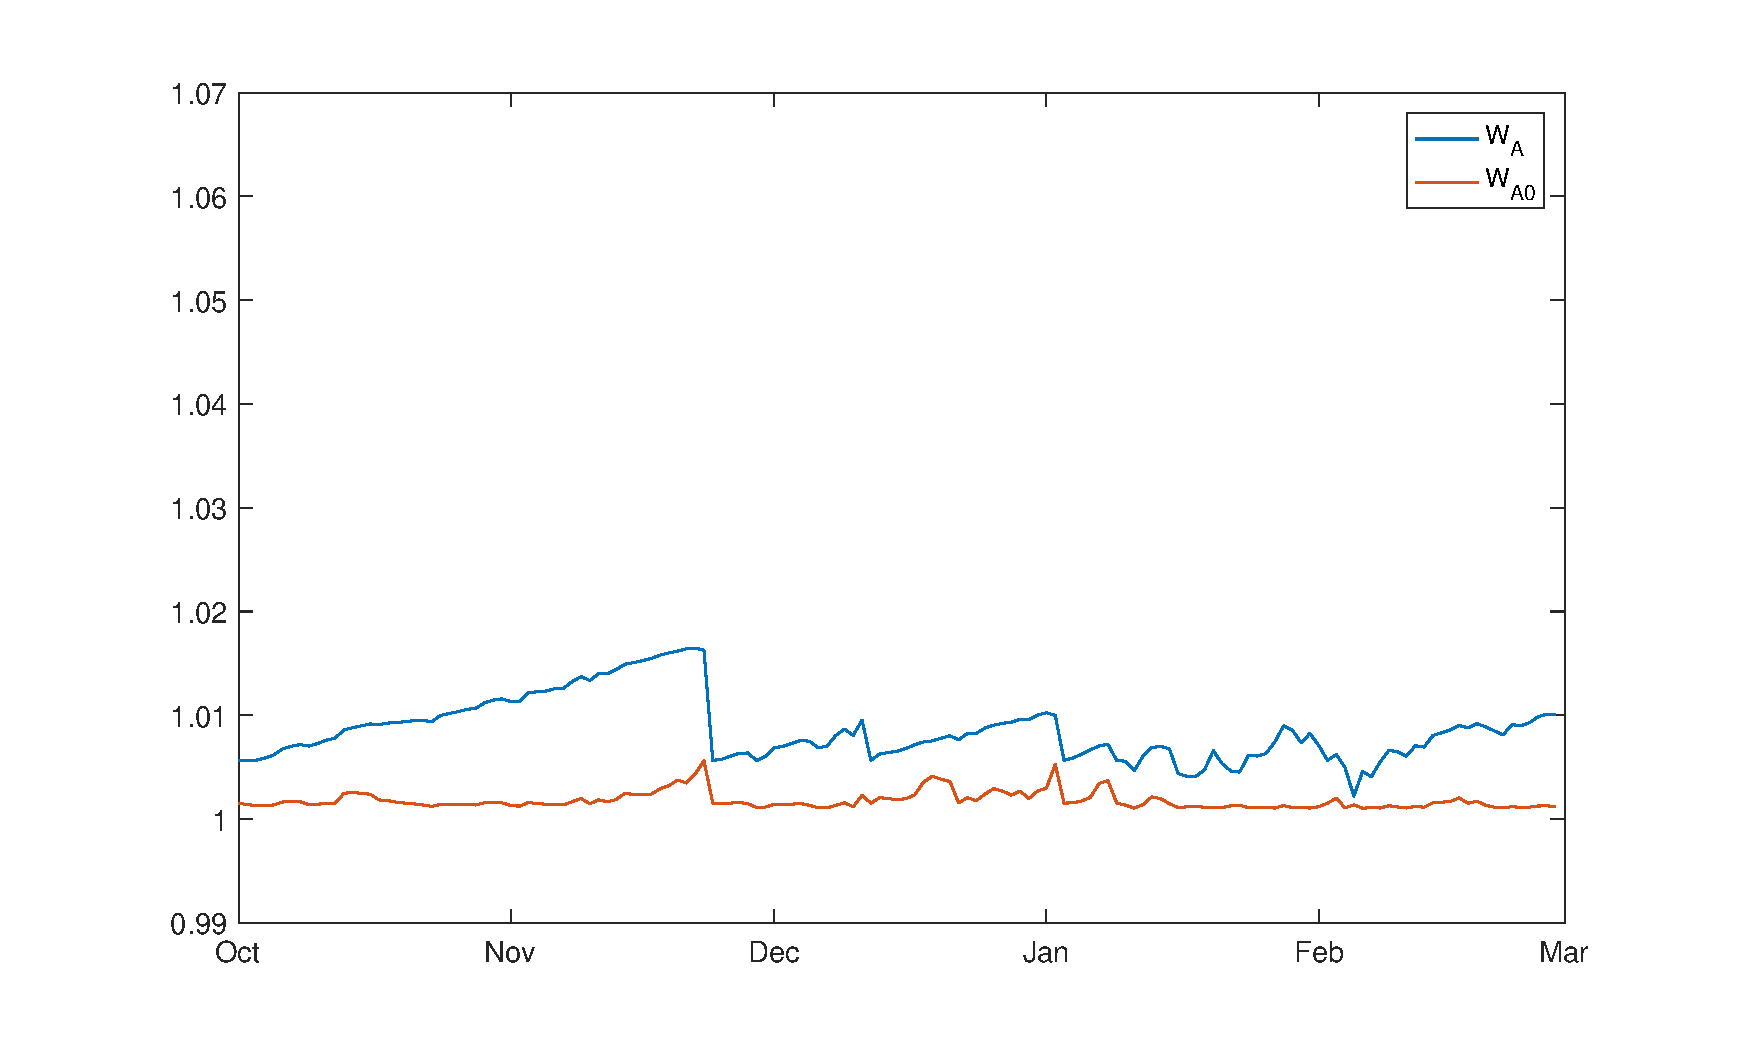
\includegraphics[width=0.9\textwidth]{WA0_alpha2.eps}
\caption{Market Value of Class A0 (principal only class) compared to Class A, where the split ratio between Class A and B coins is 2:1. Annualized volatility of Class A is 0.0125. Parameters: $R=0.02$ per day, $\mathcal{H}_{d}=0.25$, $\mathcal{H}_{u} =2$, $T=100$, $\sigma= 120\%$ per year, $r=0.0082\%$ (3\% per year). Upward reset takes place on 24 Nov 2017, 17 Dec 2017, and 7 Jan 2018. Downward reset takes place on 5 Feb 2018.}
\label{fig:valA0a2}
\end{figure}






Figure \ref{fig:valA0a1} shows the simulated path for the prices of class A0, the principal only part of A. A0 has an annualized standard deviation of 0.0412 for $\alpha=1$, as compared to that of $W_A$, which is 0.0531. Note that A0 is still volatile. To make A0 more stable, one can increase the split ratio between A and B from 1:1 to a higher split ratio $\alpha:1$, ($\alpha >1$), resulting in a lower leverage ratio for class B which in turn leads to a lower risk for Class A and Class A0, because the risk of downside resets is lower. Figure \ref{fig:valA0a2} illustrates the price of A0 with $\alpha=2$. Class A0 has an annualized standard deviation of 0.0156 for $\alpha=2$, as compared to that of $W_A$, which is 0.0571. Note that with $\alpha = 2$, the net asset value of B is $3S_t-2(1+R v_t)$, making B more sensitive to $S$.



% \section{Further Development}
% % \begin{flushright}
% % {\small{}Patience, persistence and perspiration make an unbeatable
% % combination for success.}\\
% % {\small{}\textendash{} }\emph{\small{}Napoleon Hill}
% % \par\end{flushright}{\small \par}

% This paper has outlined the main design and market mechanism for the dual-class token structure. Further studies can be done in below aspects.

% \subsubsection*{Underlying Price Pair}

% While the dual class structure is independent of the underlying crypto fiat price pair, the liquidity and popularity of the underlying price pair do impact the viability of the structure as market arbitrage is important to ensure the structure trades as designed. In this paper, ETH/USD is used as the underlying price pair, but other popular ERC20 tokens, such as EOS, ADA, paired with major fiat other than USD, can also be considered.

% % \subsubsection*{Base Rate Discovery}

% % Arbitrary rate can be used for Class A coupon and it will be traded on premium or at discount based on the market required rate of return. However, it is desirable that Class A trades close to its net value, which means the coupon rate for Class A should be chosen close to the market rate. Currently there are few observable proxies in the market. Several centralized exchanges allowing margin trading are charging USD borrow rates in the range of 20\% to 40\% per annum.

% % As discussed in Section \ref{subsec:Premium-and-Discount}, the market premium or discount of Class A token may imply USD's borrow rate in this market. As the structure gains attractions, its implied rate could serve as an indication for other USD borrow practice in crypto market.

% \subsubsection*{Optimal Reset Thresholds}

% It is important to keep leverage for Class B within certain range: not too high so as to protect Class A holders from sudden price drop and not too low so as to keep Class B attractive to leveraged users. However, it is undesirable that resets, especially downward resets, happen too frequently.

% There are two main parameters to be determined, the ratio between Class A and Class B shares, $\alpha$ (see Appendix \ref{subsec:General-Product-Design}); and the lower limit of Class B net value, $\mathcal{H}_{d}$ , that triggers downward resets. The Chinese market over the years has concluded a broadly accepted set of parameters: $\alpha$ is set to 1, meaning the quantities of Class A versus Class B is 1:1; $\mathcal{H}_{d}$ being 0.25, meaning a downward reset will be triggered if the underlying price dropped approximately 37.5\% from last reset. This setup has been tested in extreme market events such as the mid-2015 market crash and the early-2016 circuit breaker turmoil, where the reset clauses were all successfully implemented and protected the interests of Class A holders.

% We witness that cryptocurrencies have considerably higher volatility than stock market indices. A series of back testings and Monte Carlo simulations will be performed to investigate the optimal parameters for dual class token structures.

\end{appendices}



%\bibliography{Token1}
%  \newpage


%\section*{\clearpage{}}
% \begin{thebibliography}{1}

% \bibitem[1]{AC}Adams, A. T., and J. B. Clunie. 2006. Risk Assessment Techniques for Split Capital Investment Trusts. \textit{Annals of Actuarial Science} 1:7-36.

% \bibitem[2]{Basecoin}Basecoin: A Price-Stable Cryptocurrency with an Algorithmic Central Bank. \textit{\href{http://www.getbasecoin.com/basecoin_whitepaper_0_99.pdf}{http://www.getbasecoin.com/basecoin\_{}whitepaper\_{}0\_{}99.pdf}}

% \bibitem[3]{GRod3}Bech, M. L. and Garratt, R. 2017. Central Bank Cryptocurrencies. \textit{BIS Quarterly Review September 2017}. Available at SSRN: \textit{\href{https://ssrn.com/abstract=3041906}https://ssrn.com/abstract=3041906}.

% \bibitem[4]{BS}Black, F., and M. Scholes. 1973. The Pricing of Options and Corporate Liabilities. \textit{Journal of Political Economy} 81:637-654.

% \bibitem[5]{DM2018}Dai, M., S. Kou, C. Yang, and Z. Ye. 2018. The Overpricing of Leveraged Products: A Case Study of Dual-Purpose Funds in China. \textit{Working Paper}.

% \bibitem[6]{Dai:2016vj}Dai, M., S. Kou, and C. Yang. 2017. A Stochastic Representation for Nonlocal Parabolic PDEs with Applications. \textit{Working Paper}.

% \bibitem[7]{GRod}Garratt, R. 2016. CAD-coin versus Fedcoin. R3 Report 15.

% \bibitem[8]{GRod2}Garratt, R., Wallace, N. 2017. Bitcoin 1, Bitcoin 2, ...: An Experiment in Privately Issued Outside Monies. \textit{Economic Inquiry}, forthcoming.

% \bibitem[9]{Grinberg}Grinberg, R. 2011. Bitcoin: An Innovative Alternative Digital Currency. \textit{Hastings Science \& Technology Law Journal}, 4:159-208. Available at SSRN: \textit{\href{https://ssrn.com/abstract=1817857}https://ssrn.com/abstract=1817857}.

% \bibitem[10]{Harvey}Harvey, C. 2016. Cryptofinance. Available at SSRN: \textit{\href{https://ssrn.com/abstract=2438299}https://ssrn.com/abstract=2438299}.

% \bibitem[11]{Ingersoll1976}Ingersoll, J. E. 1976. A Theoretical and Empirical Investigation of the Dual Purpose Funds: an Application of Contingent-claims Analysis. \textit{Journal of Financial Economics} 3:83-123.

% \bibitem[12]{JO}Jarrow, R. A., and M. O'Hara. 1989. Primes and Scores: An Essay on Market Imperfections. \textit{The Journal of Finance} 44:1263-1287.

% \bibitem[13]{Nakamoto}Nakamoto, S. 2008. Bitcoin: A peer-to-peer electronic cash system. \textit{\href{https://bitcoin.org/bitcoin.pdf}https://bitcoin.org/bitcoin.pdf}

% \bibitem[14]{Rogoff}Rogoff, K. 2015. Costs and benefits to phasing out paper currency. \textit{NBER Macroeconomics Annual}, 29(1):445-456.

% \bibitem[15]{USDT}Tether: Fiat currencies on the Bitcoin blockchain. \textit{\href{https://tether.to/wp-content/uploads/2016/06/TetherWhitePaper.pdf}{https://tether.to/wp-content/uploads/2016/06/TetherWhitePaper.pdf}}

% \bibitem[16]{MAKERDAO}The Dai Stablecoin System. \textit{\href{https://makerdao.com/whitepaper/DaiDec17WP.pdf}{https://makerdao.com/whitepaper/DaiDec17WP.pdf}}

% \bibitem[17]{ETH}The White Paper of Ethereum: A Next-Generation Smart Contract and Decentralized Application Platform. \textit{\href{https://github.com/ethereum/wiki/wiki/White-Paper}{https://github.com/ethereum/wiki/wiki/White-Paper}}



% \end{thebibliography}

\end{document}
